\documentclass[11pt,a4paper]{article}
\usepackage{fontawesome5}
\usepackage{xcolor}

\usepackage[cache=false]{minted}
\usepackage[T1]{fontenc}
\usepackage[utf8]{inputenc}
\usepackage{lmodern}
\usepackage{microtype}
\usepackage{graphicx}
\usepackage{float}
\usepackage{amsmath,amssymb}
\usepackage{booktabs}
\usepackage{setspace}
\pagestyle{empty}
\usepackage{multirow}
\usepackage{tikz}
\usetikzlibrary{arrows.meta,positioning,calc,shapes.geometric,fit,backgrounds}
\usepackage{pgfplots}
\pgfplotsset{compat=1.18}
\usepgfplotslibrary{groupplots,fillbetween}
\usepackage{pgfplotstable}
\usepackage{tabularx}
\usepackage{array}
\usepackage{xcolor}
\usepackage{eurosym}
\usepackage{multicol}
\usepackage{enumitem}
\usepackage{mdframed}
\usepackage{adjustbox}
\usepackage{longtable}
\usepackage{pgfmath}
\usepackage{collcell}
\usepackage{minted} % explicit


\DeclareUnicodeCharacter{2061}{}
\DeclareUnicodeCharacter{00B7}{\ensuremath{\cdot}}
\DeclareUnicodeCharacter{2014}{--}
\DeclareUnicodeCharacter{2191}{\ensuremath{\uparrow}}
\DeclareUnicodeCharacter{2192}{\ensuremath{\rightarrow}}
\DeclareUnicodeCharacter{2193}{\ensuremath{\downarrow}}
\DeclareUnicodeCharacter{25C4}{\ensuremath{\blacktriangleleft}}
\DeclareUnicodeCharacter{25BA}{\ensuremath{\blacktriangleright}}
\usetikzlibrary{positioning}

% ── Figure colour palette (edit these to restyle all figures at once) ────────
\definecolor{fignavy}{HTML}{1A3A5C}
\definecolor{figblue}{HTML}{4A7FB5}
\definecolor{figlblue}{HTML}{DCE8F5}
\definecolor{figred}{HTML}{C0392B}
\definecolor{figgreen}{HTML}{1E8449}
\definecolor{figgrey}{HTML}{555555}
\definecolor{figmgrey}{HTML}{F0F0F0}
\definecolor{figgold}{HTML}{D4A017}
\newcommand{\edit}[1]{#1}

\def\MintedPygmentize{/usr/bin/pygmentize}
\PassOptionsToPackage{table}{xcolor}
% ── Shared pgfplots style ────────────────────────────────────────────────────
\pgfplotsset{
  fig style/.style={
    font=\small,
    axis line style={fignavy, line width=0.6pt},
    tick style={fignavy},
    tick label style={color=figgrey},
    label style={color=figgrey},
    title style={color=fignavy, font=\small\bfseries},
    grid=none,
    axis x line*=bottom,
    axis y line*=left,
  }
}

\setlength{\parindent}{0em}
\setlength{\parskip}{0.3em}
\setstretch{1.05}

% =========================================================
\usepackage[a4paper,top=58pt,bottom=70pt,left=54pt,right=55pt]{geometry}
\usepackage{titlesec}

% =========================================================
% Colours
% =========================================================
\definecolor{ucdblue}{RGB}{0,0,179}
\definecolor{accentred}{RGB}{180,45,45}

\setlength{\columnsep}{24pt}
\setlength{\parindent}{0em}
\setlength{\parskip}{0pt}

\onehalfspacing



% -- SSMS-ish colours --
\definecolor{sqlKW}{HTML}{0000FF}   % keywords (blue)
\definecolor{sqlFN}{HTML}{FF00FF}   % built-in funcs (magenta)
\definecolor{sqlSTR}{HTML}{A31515}  % strings (dark red)
\definecolor{sqlCOM}{HTML}{008000}  % comments (green)
\definecolor{sqlLN}{HTML}{7A7A7A}   % line numbers (grey)
\definecolor{PolyBlue}{RGB}{30,80,162}
\definecolor{ForestGreen}{RGB}{34,139,34}


\setminted{
  style=vs,
  fontsize=\small,
  breaklines,
  breakanywhere,
  autogobble,
  tabsize=4
}

\usepackage{listings}

\lstset{
    basicstyle=\small\ttfamily,
    keywordstyle=\color{sqlKW}\bfseries,
    commentstyle=\color{sqlCOM}\itshape,
    stringstyle=\color{sqlSTR},
    numberstyle=\tiny\color{sqlLN},
    identifierstyle=\color{black},
    emphstyle=\color{sqlFN},
    breaklines=true,
    breakatwhitespace=false,
    showstringspaces=false,
    tabsize=4,
    captionpos=b,
    frame=single,
    framesep=3pt,
    rulecolor=\color{gray!30},
    xleftmargin=0.5em,
    xrightmargin=0.5em,
    aboveskip=0.8em,
    belowskip=0.6em,
    columns=fullflexible,
    keepspaces=true,
    upquote=true,
}

% ------- Maths -------
\usepackage{amsmath, amssymb, amsthm, mathtools}
\makeatletter
\@removefromreset{equation}{section}
\makeatother
\renewcommand{\theequation}{\arabic{equation}}

% ------- Lists -------
\setlist{itemsep=2pt,topsep=4pt}
\usepackage[hidelinks]{hyperref}
\hypersetup{colorlinks=true, linkcolor=blue, citecolor=black, urlcolor=blue}

\setlength{\parindent}{0pt}
\renewcommand{\arraystretch}{1.2}

% Convenience column types
\newcolumntype{L}{>{\raggedright\arraybackslash}X}
\newcolumntype{C}{>{\centering\arraybackslash}m{0.22\linewidth}}

% Graphics path (for the one remaining PNG: cold_start_evaluation)


% =========================================================
% Centralised report constants (synced to saved notebook outputs)
% =========================================================
\newcommand{\ColdAllRows}{\edit{22,752}}
\newcommand{\ColdAllEdge}{\edit{0.0023}}
\newcommand{\ColdAllHit}{\edit{0.5334}}
\newcommand{\ColdAllProb}{\edit{0.5311}}
\newcommand{\DivTopRows}{\edit{2,276}}
\newcommand{\DivTopEdge}{\edit{0.0059}}
\newcommand{\DivTopHit}{\edit{0.2377}}
\newcommand{\DivTopProb}{\edit{0.2318}}
\newcommand{\MainTopRows}{\edit{2,276}}
\newcommand{\MainTopEdge}{\edit{0.2090}}
\newcommand{\MainTopHit}{\edit{0.7443}}
\newcommand{\MainTopProb}{\edit{0.5353}}
\newcommand{\PriceTopRows}{\edit{2,279}}
\newcommand{\PriceTopEdge}{\edit{0.0114}}
\newcommand{\PriceTopHit}{\edit{0.9952}}
\newcommand{\PriceTopProb}{\edit{0.9838}}
\newcommand{\FilteredRows}{\edit{2,195}}
\newcommand{\FilteredEdge}{\edit{0.2137}}
\newcommand{\MeanTradePnl}{\edit{65.38}}
\newcommand{\StdTradePnl}{\edit{211.01}}
\newcommand{\TradeSharpe}{\edit{0.396}}
\newcommand{\TradeVaR}{\edit{153.98}}
\newcommand{\TradeCVaR}{\edit{370.83}}
\newcommand{\MaxDrawdownUSD}{\edit{16,040.47}}
\newcommand{\MaxDrawdownPct}{\edit{11.2}}
\newcommand{\GrossPnlSevenMonths}{\edit{143,506.58}}
\newcommand{\TradesPerMonth}{\edit{314}}
\newcommand{\PeakCapitalUSD}{\edit{156,786}}
\newcommand{\AnnualPnlOneM}{\edit{246,011}}
\newcommand{\AnnualPnlFiveM}{\edit{1,205,455}}
\newcommand{\AnnualPnlTenM}{\edit{2,214,101}}
\newcommand{\NetTeamOneM}{\edit{252,212}}
\newcommand{\NetTeamFiveM}{\edit{636,162}}
\newcommand{\NetTeamTenM}{\edit{1,570,094}}
\newcommand{\FiveMScale}{\edit{4.9}}
\newcommand{\TenMScale}{\edit{9.0}}

% =========================================================
% Section 1 (wallet EDA) constants — re-populated after a fresh
% run of wallet_Analysis_v2.ipynb. Macros match the pattern used
% above so the tex compiles cleanly before the notebook is re-run.
% =========================================================
\newcommand{\RawUniqueWallets}{\edit{333{,}124}}
\newcommand{\MedTradesPerWallet}{\edit{6}}
\newcommand{\PSeventyFiveTradesPerWallet}{\edit{14}}
\newcommand{\PNinetyNineTradesPerWallet}{\edit{316}}
\newcommand{\TopfVolumeShare}{\edit{39.7}}
\newcommand{\WalletsHalfVolume}{\edit{132}}
\newcommand{\ExpWallets}{\edit{16{,}661}}
\newcommand{\ExpWalletsPct}{\edit{5.1}}
\newcommand{\ExpMedianHit}{\edit{55.6}}
\newcommand{\ExpPsfHit}{\edit{75.7}}
\newcommand{\ExpWalletsAboveSixtyFive}{\edit{6{,}059}}
\newcommand{\WhaleQuadrantCount}{\edit{1{,}422}}
\newcommand{\WhaleVolQSeventyFive}{\edit{5{,}933}}
\newcommand{\EarlyAccurateCount}{\edit{1{,}299}}
\newcommand{\EarlyThresholdDays}{\edit{64}}
% Bootstrap CIs (95%, wallet-clustered, 3,000 iterations)
\newcommand{\MedianHitCI}{\edit{[54.6,\,56.3]}}
\newcommand{\TopfShareCI}{\edit{[38.9,\,40.5]}}
\newcommand{\WhaleCountCI}{\edit{[1{,}349,\,1{,}493]}}
% Realised-edge EDA
\newcommand{\WhaleMeanEdge}{\edit{0.152}}
\newcommand{\WhaleMeanEdgeCI}{\edit{[0.146,\,0.158]}}
\newcommand{\AllWalletMeanEdge}{\edit{0.121}}
% Herfindahl
\newcommand{\HhiMedian}{\edit{0.079}}
\newcommand{\HhiTopDecile}{\edit{0.115}}
% Survival into cold-start window (Sep 2025 - Apr 2026)
\newcommand{\WhaleSurvivalCount}{\edit{925}}
\newcommand{\WhaleSurvivalPct}{\edit{65.0}}
% Label construction
\newcommand{\PositiveLabels}{\edit{614}}
\newcommand{\PositiveLabelsFromWhaleShare}{71.3}
% Threshold sensitivity
\newcommand{\ExpWalletsAtFive}{\edit{46{,}328}}
\newcommand{\ExpWalletsAtTwenty}{\edit{5{,}719}}
\newcommand{\MedianHitAtFive}{\edit{60.0}}
\newcommand{\MedianHitAtTwenty}{\edit{54.1}}

% =========================================================
% Alternating side page-number badges
% =========================================================
\newcommand{\DrawPageBadgeAndNumber}{%
\begin{tikzpicture}[remember picture,overlay]
  \ifnum\value{page}<50
    \ifodd\value{page}
      \fill[ucdblue]
        ([yshift=278pt]current page.south west)
        rectangle
        ([xshift=40pt,yshift=318pt]current page.south west);
      \node[white,font=\sffamily\bfseries\fontsize{18}{18}\selectfont]
        at ([xshift=20pt,yshift=296.346pt]current page.south west) {\thepage};
    \else
      \fill[ucdblue]
        ([xshift=-40pt,yshift=278pt]current page.south east)
        rectangle
        ([yshift=318]current page.south east);
      \node[white,font=\sffamily\bfseries\fontsize{18}{18}\selectfont]
        at ([xshift=-20pt,yshift=296.346pt]current page.south east) {\thepage};
    \fi
  \else
    \node[black,font=\fontsize{9}{9}\selectfont]
      at ([yshift=14pt]current page.south) {\thepage};
  \fi
\end{tikzpicture}%
}
\AddToHook{shipout/foreground}{\DrawPageBadgeAndNumber}

% =========================================================
% Front hero block
% =========================================================
\newcommand{\FrontHero}{%
\begin{tikzpicture}[remember picture,overlay]
  \node[anchor=north west,inner sep=0]
    at ([yshift=-46pt]current page.north west)
    {\includegraphics[width=\paperwidth,height=292pt]{here-top}};
  \fill[ucdblue,opacity=0.80]
    ([xshift=94pt,yshift=-38pt]current page.north west)
    rectangle
    ([xshift=491pt,yshift=-362pt]current page.north west);
  \node[anchor=north west,inner sep=0]
    at ([xshift=143pt,yshift=-95pt]current page.north west)
    {\includegraphics[width=147pt]{Smurfit colour transparent.png}};
  \node[anchor=north,align=center,text=white,font=\bfseries\fontsize{17}{18}\selectfont]
    at ([xshift=292pt,yshift=-57pt]current page.north west)
    {FIN42110: FDS for Trading \& Risk\\[0.65em] Group Assignment};
  \node[anchor=north,align=center,text=white,font=\fontsize{13}{15}\selectfont]
    at ([xshift=292pt,yshift=-122pt]current page.north west)
    {Group 7};
  \node[anchor=north west,text=white,align=left,text width=360pt,font=\fontsize{10.8}{12.2}\selectfont]
    at ([xshift=108pt,yshift=-163pt]current page.north west)
    {\edit{We study whether wallet behaviour, textual signals, and broader market context can identify mispriced Polymarket trades in geopolitical prediction markets. EDA shows a highly concentrated market in which a small minority of wallets accounts for a disproportionate share of volume and strong historical hit rates. We then frame a cold-start ML task that requires the model to generalise to wallets never seen in training. A tuned XGBoost model using price, context, and sentiment features improves on the market-price baseline on unseen wallets, with held-out ROC-AUC rising from 0.9432 to 0.9534 and uplift across ranking and calibration metrics. The economic value comes from screening rather than trading everything: the top-decile alpha slice delivers materially higher realised edge. It remains positive under real-world scenario, useful for decision-support with tight liquidity and sizing controls rather than full automation.}};
\end{tikzpicture}
\vspace*{338pt}}


\begin{document}

%\vspace{-7.5em}
\tableofcontents

%\begin{table}[H]
%\centering
%\begin{tabular}{l | c}
%\toprule
%Section 1 & -  \\[0.25em]
%Section 2 & -  \\[0.25em]
%Section 3 & -  \\[0.25em]
%Section 4 & -   \\[0.25em]
%\midrule
%Total words (including everything) & - \\
%\bottomrule
%\end{tabular}
%\caption{Word Count Summary (using \href{https://quillbot.com/word-counter}{Quillbot})}
%\end{table}

\newpage

\begin{tabularx}{\textwidth}{>{\bfseries}l L >{\bfseries}l L}
\toprule
Student Name 1 & Andrew Holton     & Student Number 1 & 25224517  \\
Student Name 2 & John Stewart      & Student Number 4 & 25210841  \\
Student Name 3 & Ois\'{i}n Moffatt & Student Number 3 & 21510573  \\
Student Name 4 & Adam Ajmal        & Student Number 5 & 20309543  \\
Module Title & FIN42110: FDS for Trading \& Risk Mgmt & Module Co-ordinator & Dr Richard McGee \\
\bottomrule
\end{tabularx}

\vspace{1.2cm}

{\bfseries Procedures for Submission and Late Submission:} ensure that you have checked the School's procedures for the submission of assessments. Note: There are penalties for the late submission of assessments. For further information please see the University's Policy on Late Submission of Coursework, \href{http://www.ucd.ie/registrar/}{(http://www.ucd.ie/registrar/)}.

\vspace{0.7cm}

{\bfseries Plagiarism:} the unacknowledged inclusion of another person's writings or ideas or works, in any formally presented work (including essays, examinations, projects, laboratory reports or presentations). The penalties associated with plagiarism are designed to impose sanctions that reflect the seriousness of University's commitment to academic integrity. Ensure that you have read the University's Briefing for Students on Academic Integrity and Plagiarism and the UCD Plagiarism Statement, Plagiarism Policy and Procedures, \href{http://www.ucd.ie/registrar/}{(http://www.ucd.ie/registrar/)}.

\vspace{0.7cm}

{\bfseries Declaration of Authorship}

We declare that all material in this assessment is our own work except where there is clear acknowledgement and appropriate reference to the work of others.

\vspace{0.4cm}
Signed \dotfill Andrew Holton \dotfill

\vspace{0.3cm}
Signed \dotfill Ois\'{i}n Moffatt \dotfill

\vspace{0.3cm}
Signed \dotfill John Stewart \dotfill

\vspace{0.3cm}
Signed \dotfill Adam Ajmal \dotfill

\newpage

\begin{center}
\vspace{1.2em}
{\large \faGithub\;
\href{https://github.com/johnstew324/polymarket-whale-watch}{%
\texttt{johnstew324/polymarket-whale-watch}}}
\end{center}

% ── 2.1 Data Source Evaluation ───────────────────────────────────────────────
\section{Data Source Evaluation}
\label{sec:data_sources}

Polymarket is a decentralised prediction market built on Polygon,
a proof-of-stake Ethereum sidechain \cite{polymarket_docs}. Users can
trade on the outcomes of real-world events using USDC as
collateral. The technical structure of these markets is defined by:

\begin{itemize}
    \item \textbf{Market Mechanics:} Each market generates a pair of binary outcome tokens \texttt{YES}/\texttt{NO}. These outcomes are priced between \$0 and \$1, which  directly reflects the market's implied probability of these event occurring.
    \item \textbf{Token Standards:} Each binary outcome is implemented as \textbf{ERC-1155} assets - fungible tokens with 6-decimal precision, traded in discrete units. 
    \item \textbf{Settlement and Transparency:} All trades are settled through the CTF Exchange smart contract and are permanently recorded on-chain as \texttt{OrderFilled} events.
    \item \textbf{Data Accessibility:} both counterparty wallet addresses are therefore
    publicly visible in every event, making the full trade history queryable directly from the blockchain.
\end{itemize}


\subsubsection*{Trade History Acquisition:}
Obtaining the history at wallet level and at scale required evaluating
many sources of data, However several alternative data sources were evaluated and rejected, i.e. the Polymarket Data API, Dune Analytics,
 Allium, CryptoHouse, and Goldsky. These sources were unsuitable because they either 
 imposed restrictive data caps, required paid or enterprise access, lacked Polymarket 
 coverage, or omitted the wallet-level fields needed for this analysis.

\paragraph{Chosen source: S3 snapshot of on-chain events.}


The complete \texttt{OrderFilled} event history was taken from the community-maintained S3 archive published by 
\texttt{warproxxx/poly\_data}~\cite{poly_data_github}, rather than scraped live. This was used because rebuilding the 
2023--2025 history via GraphQL pagination takes over two days, making the snapshot a more practical choice for 
validating the modelling approach. Extending the dataset beyond October 2025 through a live pipeline remains a possible future
 improvement. Table~\ref{tab:s3_snapshot} summarises the final dataset.

\vspace{0.6em}
\begin{table}[H]
\centering
\caption{S3 snapshot properties.}
\label{tab:s3_snapshot}
\small
\begin{tabularx}{\textwidth}{l X}
\toprule
\textbf{Property} & \textbf{Value} \\
\midrule
File                & \texttt{orderFilled\_complete.csv.xz} \\
Compressed size     & 5.9\,GB \\
Uncompressed size   & $\sim$35--40\,GB \\
Total rows          & 150M$+$ \\
Date range          & 1 February 2023 - 7 October 2025 \\
Hosted at           & \texttt{polydata-archive.s3.us-east-1.amazonaws.com} \\
\bottomrule
\end{tabularx}
\end{table}

\newpage
% ── 2.2 Pipeline Architecture ─────────────────────────────────────────────────
\subsection{Pipeline Architecture}
\label{sec:pipeline}

The data collection pipeline consists of a snapshot download followed
by five Python modules executed sequentially, with each step's output
feeding directly into the next.
Figure~\ref{fig:pipeline} shows the full flow from the S3 archive and
external APIs through to the analytical DuckDB database.
Full setup and reproduction instructions are provided in the project
\texttt{README.md}\footnote{\href{https://github.com/johnstew324/polymarket-whale-watch}{%
\faGithub\;\texttt{johnstew324/polymarket-whale-watch}}}


\begin{figure}[H]
\centering
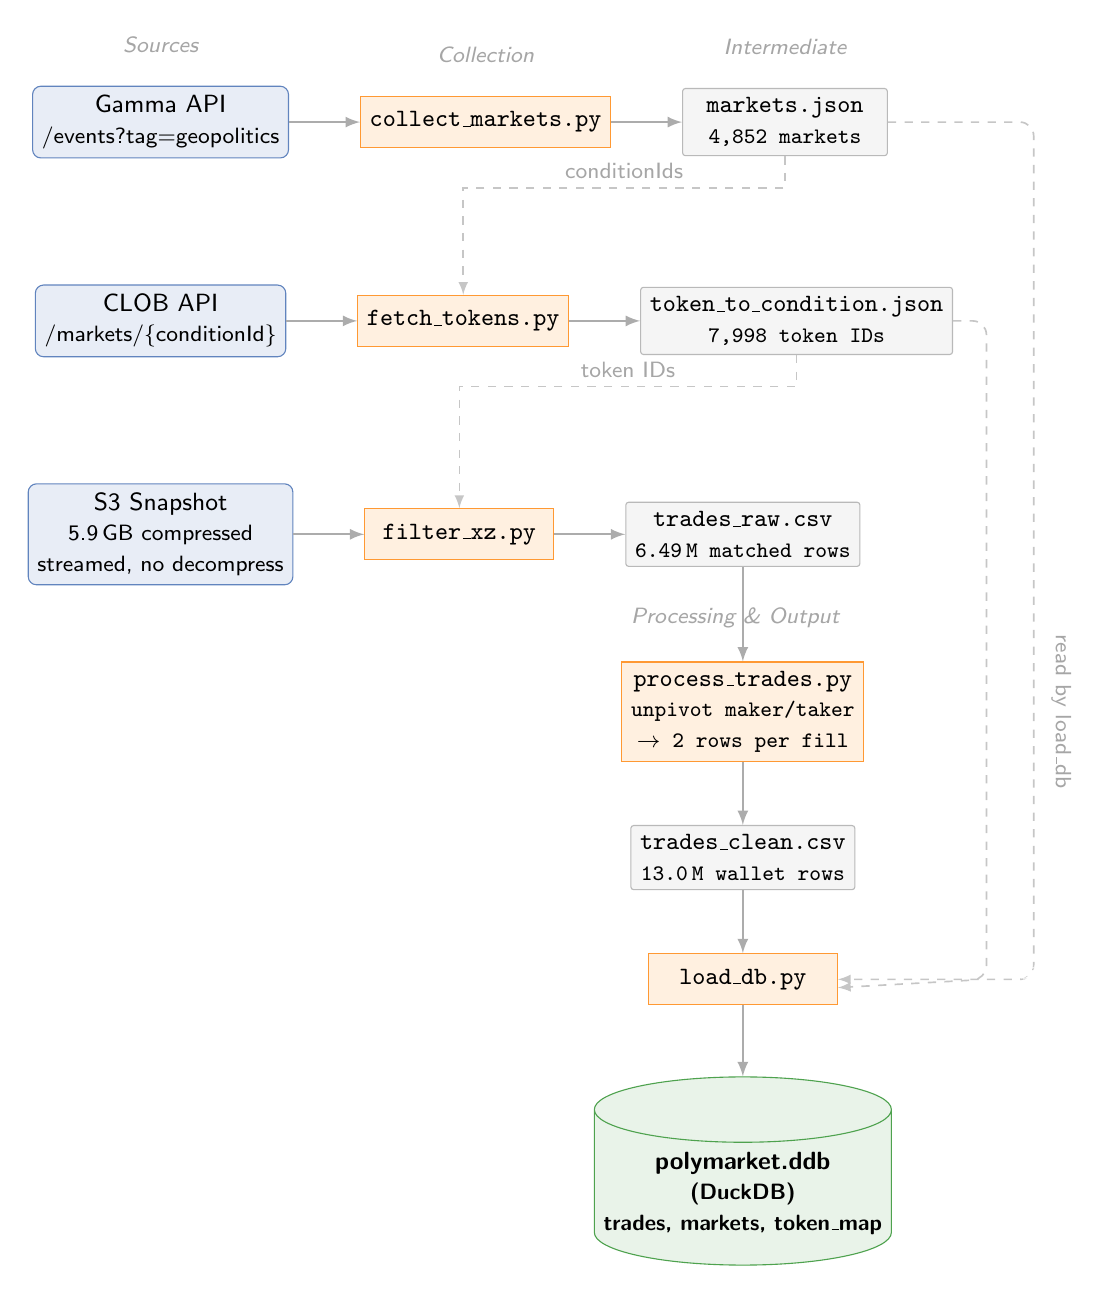
\begin{tikzpicture}[
    node distance = 0.6cm and 0.9cm,
    % ── Node styles ──
    api/.style   = {rectangle, rounded corners=3pt,
                    draw=PolyBlue!70, fill=PolyBlue!10,
                    minimum width=2.4cm, minimum height=0.7cm,
                    font=\small\sffamily, align=center},
    script/.style= {rectangle,
                    draw=orange!80, fill=orange!12,
                    minimum width=2.4cm, minimum height=0.65cm,
                    font=\small\ttfamily, align=center},
    file/.style  = {rectangle, rounded corners=1pt,
                    draw=gray!55, fill=gray!8,
                    minimum width=2.6cm, minimum height=0.65cm,
                    font=\small\ttfamily, align=center},
    db/.style    = {cylinder, shape border rotate=90, aspect=0.22,
                    draw=ForestGreen!80, fill=ForestGreen!10,
                    minimum width=2.6cm, minimum height=0.9cm,
                    font=\small\sffamily\bfseries, align=center},
    arr/.style   = {->, >=latex, thick, gray!65},
    dep/.style   = {->, >=latex, semithick, gray!45, dashed},
    arrlbl/.style= {font=\footnotesize\sffamily, text=gray!70, fill=white, inner sep=2pt},
    labl/.style  = {font=\footnotesize\sffamily\itshape, text=gray!70},
]

% =====================================================================
%  ROW 1: Gamma API → collect_markets.py → markets.json
% =====================================================================
\node[api] (gamma) {Gamma API\\
    {\footnotesize /events?tag=geopolitics}};
\node[script, right=0.9cm of gamma] (cm) {collect\_markets.py};
\node[file, right=0.9cm of cm] (mj) {markets.json\\
    {\footnotesize 4{,}852 markets}};

\draw[arr] (gamma) -- (cm);
\draw[arr] (cm)    -- (mj);

% =====================================================================
%  ROW 2: CLOB API → fetch_tokens.py → token_to_condition.json
% =====================================================================
\node[api, below=1.6cm of gamma] (clob) {CLOB API\\
    {\footnotesize /markets/\{conditionId\}}};
\node[script, right=0.9cm of clob] (ft) {fetch\_tokens.py};
\node[file, right=0.9cm of ft] (tc) {token\_to\_condition.json\\
    {\footnotesize 7{,}998 token IDs}};

\draw[arr] (clob) -- (ft);
\draw[arr] (ft)   -- (tc);

% ── markets.json → fetch_tokens (conditionIds flow down)
\draw[dep] (mj.south) -- ++(0,-0.4) coordinate (cid-horiz) -| (ft.north);
\node[arrlbl, above=1pt] at ($(cid-horiz)!0.5!(cid-horiz -| ft.north)$) {conditionIds};

% =====================================================================
%  ROW 3: S3 Snapshot → filter_xz.py → trades_raw.csv
% =====================================================================
\node[api, below=1.6cm of clob] (s3) {S3 Snapshot\\
    {\footnotesize 5.9\,GB compressed}\\
    {\footnotesize streamed, no decompress}};
\node[script, right=0.9cm of s3] (fx) {filter\_xz.py};
\node[file, right=0.9cm of fx] (tr) {trades\_raw.csv\\
    {\footnotesize 6.49\,M matched rows}};

\draw[arr] (s3) -- (fx);
\draw[arr] (fx) -- (tr);

% ── token_to_condition → filter_xz (token IDs flow down)
\draw[dep] (tc.south) -- ++(0,-0.4) coordinate (tid-horiz) -| (fx.north);
\node[arrlbl, above=1pt] at ($(tid-horiz)!0.5!(tid-horiz -| fx.north)$) {token IDs};

% =====================================================================
%  VERTICAL CASCADE: process → clean → load → DuckDB
%  Centred under the Intermediate column
% =====================================================================

% ── process_trades.py
\node[script, below=1.2cm of tr] (pt) {process\_trades.py\\
    {\footnotesize unpivot maker/taker}\\
    {\footnotesize $\rightarrow$ 2 rows per fill}};
\draw[arr] (tr.south) -- (pt.north);

% ── trades_clean.csv
\node[file, below=0.8cm of pt] (tc2) {trades\_clean.csv\\
    {\footnotesize 13.0\,M wallet rows}};
\draw[arr] (pt.south) -- (tc2.north);

% ── load_db.py
\node[script, below=0.8cm of tc2] (ld) {load\_db.py};
\draw[arr] (tc2.south) -- (ld.north);

% ── DuckDB
\node[db, below=0.9cm of ld] (ddb) {polymarket.ddb\\
    {\footnotesize (DuckDB)}\\
    {\footnotesize trades, markets, token\_map}};
\draw[arr] (ld.south) -- (ddb.north);

% =====================================================================
%  RIGHT-SIDE RAIL: markets.json & token_map also feed load_db
%  Use a single vertical rail at x = right edge of diagram
% =====================================================================
\coordinate (rail) at ([xshift=2.2cm]tr.east);

% markets.json → load_db (via rail)
\draw[dep, rounded corners=5pt]
    (mj.east) -- (mj.east -| rail) -- (rail |- ld.east) -- (ld.east)
    node[arrlbl, pos=0.0, above right, xshift=-4pt] {};

% token_to_condition → load_db (via rail, offset slightly)
\coordinate (rail2) at ([xshift=1.6cm]tr.east);
\draw[dep, rounded corners=5pt]
    (tc.east) -- (tc.east -| rail2) -- (rail2 |- ld.east) -- ([yshift=-3pt]ld.east);

% ── Annotations on rail
\node[arrlbl, rotate=-90, anchor=south] at ([xshift=0.15cm]rail |- pt) 
    {read by load\_db};

% =====================================================================
%  COLUMN LABELS
% =====================================================================
\node[labl, above=0.3cm of gamma] {Sources};
\node[labl, above=0.3cm of cm]    {Collection};
\node[labl, above=0.3cm of mj]    {Intermediate};
\node[labl, above=0.3cm of pt.north west, anchor=south west] {Processing \& Output};

\end{tikzpicture}
\caption{Data collection and loading pipeline. Orange: Python scripts
         (\texttt{src/pipeline/}), blue: external data sources, grey:
         intermediate files, green: analytical database.
         Solid arrows show the primary data flow; dashed arrows show
         secondary dependencies (metadata lookups).
         \texttt{filter\_xz.py} streams the S3 snapshot without full
         decompression, matching token IDs on the fly.
         Full pipeline reproducible via \texttt{make pipeline}.}
\label{fig:pipeline}
\end{figure}


\newpage

\subsubsection*{Step 0: S3 Snapshot Download:}

The first step is downloading \texttt{orderFilled\_complete.csv.xz}
into \texttt{data/raw/} from the \texttt{warproxxx/poly\_data} S3
archive (see Appendix~\ref{app:download}).

\begin{table}[H]
\centering
\caption{Example rows from \texttt{orderFilled\_complete.csv.xz}.
         Each trade assets are identified by ERC-1155 token IDs, these are
         77-digit integers assigned at market creation, one for both Yes and No.\texttt{0} denotes USDC. 
         No condition IDs or market names are present in
         the raw data, therefore the following steps of the pipeline exist to resolve this problem.}
\label{tab:raw_snapshot}
\small
\begin{tabularx}{\textwidth}{l l l r l r}
\toprule
\textbf{timestamp} & \textbf{maker} & \textbf{makerAssetId}
    & \textbf{makerAmt} & \textbf{takerAssetId} & \textbf{takerAmt} \\
\midrule
1675247746 & \texttt{0x78db{\ldots}} & \texttt{0} (USDC)
    & 29.68 & \texttt{55628{\ldots}} & 30.60 \\
1675247746 & \texttt{0xc6fd{\ldots}} & \texttt{41572{\ldots}}
    & 30.60 & \texttt{0} (USDC) & 0.92 \\
\bottomrule
\end{tabularx}
\end{table}


% ── Step 1 ────────────────────────────────────────────────────────────────────
\subsubsection*{Step 1: \texttt{collect\_markets.py}}
The pipeline begins by querying the Gamma API for all closed geopolitical markets, paginating until exhausted, and writes the result to \texttt{data/raw/markets.json}.
This file serves as the master market registry for all other steps.


\texttt{resolvedOutcome} is not returned directly by the API, it is 
derived by parsing the \texttt{outcomePrices}, string into a list and 
selecting the outcome where the price goes to \$1 at settlement. Over 5000 markets were retrieved with these parameters as of April 2026. The following table summarises the markets.json schema:

\begin{table}[H]
\centering
\caption{\texttt{markets.json} field reference.}
\label{tab:markets_schema}
\small
\begin{tabularx}{\textwidth}{l l X}
\toprule
\textbf{Field} & \textbf{Type} & \textbf{Example} \\
\midrule
\texttt{conditionId}     & string   & \texttt{0x0f99\ldots} \\
\texttt{question}        & string   & Will Putin remain President through 2024? \\
\texttt{eventTitle}      & string   & Will Putin remain President through 2024? \\
\texttt{startDate}       & ISO 8601 & \texttt{2024-03-26T15:11:43Z} \\
\texttt{endDate}         & ISO 8601 & \texttt{2024-12-31T12:00:00Z} \\
\texttt{closedTime}      & ISO 8601 & \texttt{2025-01-01T09:42:22Z} \\
\texttt{volume}          & float    & \texttt{2{,}187{,}634} \\
\texttt{outcomes}        & string[] & \texttt{["Yes", "No"]} \\
\texttt{outcomePrices}   & string[] & \texttt{["1", "0"]} \\
\texttt{resolvedOutcome} & string   & \texttt{Yes} (derived from \texttt{outcomePrices}) \\
\texttt{tags}            & string[] & \texttt{["russia", "putin", "geopolitics", \ldots]} \\
\bottomrule
\end{tabularx}
\end{table}





\subsubsection*{Step 2 \texttt{fetch\_tokens.py}}

As shown in Table~\ref{tab:raw_snapshot}, snapshot rows carry no 
conditionID (cid), only ERC-1155 token IDs. \texttt{fetch\_tokens.py} 
resolves this by querying the CLOB API for the YES/NO ERC-1155 token IDs of 
each market in \texttt{markets.json} with volume $\geq$\$1{,}000. 

\begin{figure}[H]
\centering
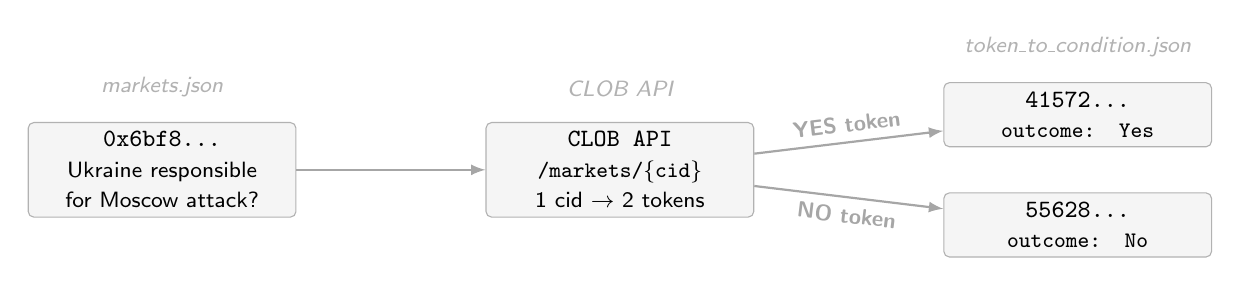
\begin{tikzpicture}[
    box/.style={rectangle, draw=gray!60, fill=gray!8, 
                rounded corners=2pt, minimum width=3.4cm, 
                minimum height=0.75cm, font=\small\ttfamily, align=center},
    arr/.style={->, >=latex, thick, gray!70},
    lbl/.style={font=\footnotesize\sffamily\itshape, text=gray!60},
    side/.style={font=\footnotesize\sffamily\bfseries, text=gray!70}
]

\node[box] (cid)  
    {\texttt{0x6bf8\ldots}\\
     {\footnotesize\sffamily Ukraine responsible}\\
     {\footnotesize\sffamily for Moscow attack?}};

\node[box, right=2.4cm of cid] (clob) 
    {CLOB API\\{\footnotesize /markets/\{cid\}}\\
     {\footnotesize\sffamily 1 cid $\rightarrow$ 2 tokens}};

\node[box, right=2.4cm of clob, yshift=0.7cm] (yes)  
    {\texttt{41572\ldots}\\{\footnotesize outcome: \textbf{Yes}}};

\node[box, right=2.4cm of clob, yshift=-0.7cm] (no)   
    {\texttt{55628\ldots}\\{\footnotesize outcome: \textbf{No}}};

\draw[arr] (cid)  -- (clob);
\draw[arr] (clob) -- node[side, above, sloped] {YES token} (yes);
\draw[arr] (clob) -- node[side, below, sloped] {NO token}  (no);

\node[lbl, above=0.2cm of cid]  {markets.json};
\node[lbl, above=0.2cm of clob] {CLOB API};
\node[lbl, above=0.2cm of yes]  {token\_to\_condition.json};

\end{tikzpicture}
\caption{Each \texttt{conditionId} is resolved to a YES and NO 
ERC-1155 token ID via the CLOB API. The token IDs shown are real 
values from the dataset.}
\label{fig:token_mapping}
\end{figure}

\noindent The \$1{,}000 volume filter excludes negligible markets,
at time of writing, \texttt{token\_to\_condition.json} contained
approximately 8,000 token IDs across 4,000 markets.





\newpage

\subsubsection*{Step 3: \texttt{filter\_xz.py}}

Using the token to condition mapping, the \texttt{filter\_xz.py} extracts matching trades from the full snapshot in a single streaming pass.
Full decompression is impractical, given the archive size
at 35-40\,GB (Table~\ref{tab:s3_snapshot}). 
\texttt{xzcat}\footnote{\url{https://linux.die.net/man/1/xzcat}} (Unix utility) is used to stream the \texttt{.xz} file line by line into a Python CSV reader, without having to write the full decompressed file to disk. 

\begin{lstlisting}[language=Python, caption={Streaming the \texttt{.xz} archive without full decompression.}, label={lst:filter_xz}]
with subprocess.Popen(["xzcat", str(IN)],
                      stdout=subprocess.PIPE,
                      bufsize=1024*1024) as proc:
    reader = csv.reader(line.decode() for line in proc.stdout)
\end{lstlisting}

\caption{Streaming the \texttt{.xz} archive without full decompression.}
\label{lst:filter_xz}
\end{listing}

\noindent Each row is checked against \texttt{token\_to\_condition.json}:
a match on either \texttt{makerAssetId} or \texttt{takerAssetId} means the row is written to the .csv file, with \texttt{condition\_id} and \texttt{outcomes} appended to that output row.

\begin{table}[H]
\centering
\caption{\texttt{trades\_raw.csv} - output of \texttt{filter\_xz.py}.}
\label{tab:trades_raw}
\small
\begin{tabularx}{\textwidth}{l X}
\toprule
\textbf{Property} & \textbf{Value} \\
\midrule
Rows           & 6,505,297 ($\approx4.3\%$ of full snapshot) \\
Unique wallets & 333,124 \\
File size      & 2.1\,GB \\
Date range     & 1 February 2023 - 7 October 2025 \\
Added columns  & \texttt{condition\_id}, \texttt{outcomes} \\
\bottomrule
\end{tabularx}
\end{table}










\subsubsection*{Step 4 \texttt{process\_trades.py}}


% TODO: INCLUDE THIS SNIPPET OR APPENDIX maker_is_buyer = row["makerAssetId"] == "0"
Each raw fill records both counterparties in one row, so
 \texttt{process\_trades.py} converts the data into wallet-level observations.
  It splits each fill into maker and taker rows, infers trade side from the asset flow,
   normalises raw amounts to USDC and token units, derives price as \texttt{usd\_amount / token\_amount}, 
   and removes dust trades with zero rounded token volume.

\begin{table}[H]
\centering
\caption{Sample rows from \texttt{trades\_clean.csv}. Each original
         fill becomes two rows with opposite sides.}
\label{tab:clean_sample}
\small
\begin{tabularx}{\textwidth}{l l l l r r r}
\toprule
\textbf{timestamp} & \textbf{wallet} & \textbf{side} &
\textbf{outcome} & \textbf{usd} & \textbf{tokens} & \textbf{price} \\
\midrule
2023-02-01 & \texttt{0x78db{\ldots}} & BUY  & No  & 29.68 & 30.60 & 0.97 \\
2023-02-01 & \texttt{0x4bfb{\ldots}} & SELL & No  & 29.68 & 30.60 & 0.97 \\
2023-02-01 & \texttt{0xc6fd{\ldots}} & BUY  & Yes &  0.92 & 30.60 & 0.03 \\
2023-02-01 & \texttt{0x78db{\ldots}} & SELL & Yes &  0.92 & 30.60 & 0.03 \\
\bottomrule
\end{tabularx}
\end{table}


  
\subsubsection*{Step 5: \texttt{load\_db.py}}

\texttt{load\_db.py} is the final step of the core pipeline, loading the
\texttt{trades\_clean.csv} and \texttt{markets.json} into a single
DuckDB analytical database (\texttt{polymarket.ddb}).
Unix timestamps are converted into native \texttt{TIMESTAMP} columns, the
\texttt{tags} field is converted from a raw JSON string to a native
\texttt{VARCHAR[]} array.
The token map is kept as a \texttt{token\_map} table for possible future
cross-reference.


% ── 2.3 Database Schema ───────────────────────────────────────────────────────
\subsection{Database Schema}
\label{sec:schema}

All pipeline outputs are stored in a single DuckDB database (\texttt{polymarket.ddb}). 
DuckDB was chosen because its columnar engine handles large aggregations efficiently, 
it supports arrays natively for storing market tags, and it remains fully portable as a
 single-file database~\cite{duckdb}.

\noindent The database contains five tables, summarised in
Table~\ref{tab:rowcounts}.  Three are loaded by the core pipeline
(\texttt{load\_db.py}): \texttt{trades}, \texttt{markets}, and
\texttt{token\_map}.  Two further tables, \texttt{sentiment} and
\texttt{financial} are both populated by the sentiment pipeline
(Section~\ref{sec:sentiment}) and joined to the core tables by the shared foreign key,
\texttt{condition\_id}.

\begin{table}[H]
\centering
\caption{Database tables after the full pipeline.}
\label{tab:rowcounts}
\small
\begin{tabularx}{\textwidth}{l r X}
\toprule
\textbf{Table} & \textbf{Rows} & \textbf{Loaded by} \\
\midrule
\texttt{trades}     & 13{,}010{,}594 & \texttt{load\_db.py} \\
\texttt{markets}    &      5{,}372   & \texttt{load\_db.py} \\
\texttt{token\_map} &      8{,}794   & \texttt{load\_db.py} \\
\texttt{sentiment}  &        ---     & sentiment pipeline
                                       (Section~\ref{sec:sentiment}) \\
\texttt{financial}  &        ---     & sentiment pipeline
                                       (Section~\ref{sec:sentiment}) \\
\bottomrule
\end{tabularx}
\end{table}

\noindent Figure \ref{fig:schema} shows the full schema and
relationships between tables.  \texttt{condition\_id} is the shared
foreign key that links trade activity, market metadata, token
identifiers, and the sentiment and financial enrichment layers.

% ── Schema diagram ───────────────────────────────────────────────────────────
\begin{figure}[H]
\centering
\resizebox{\textwidth}{!}{%
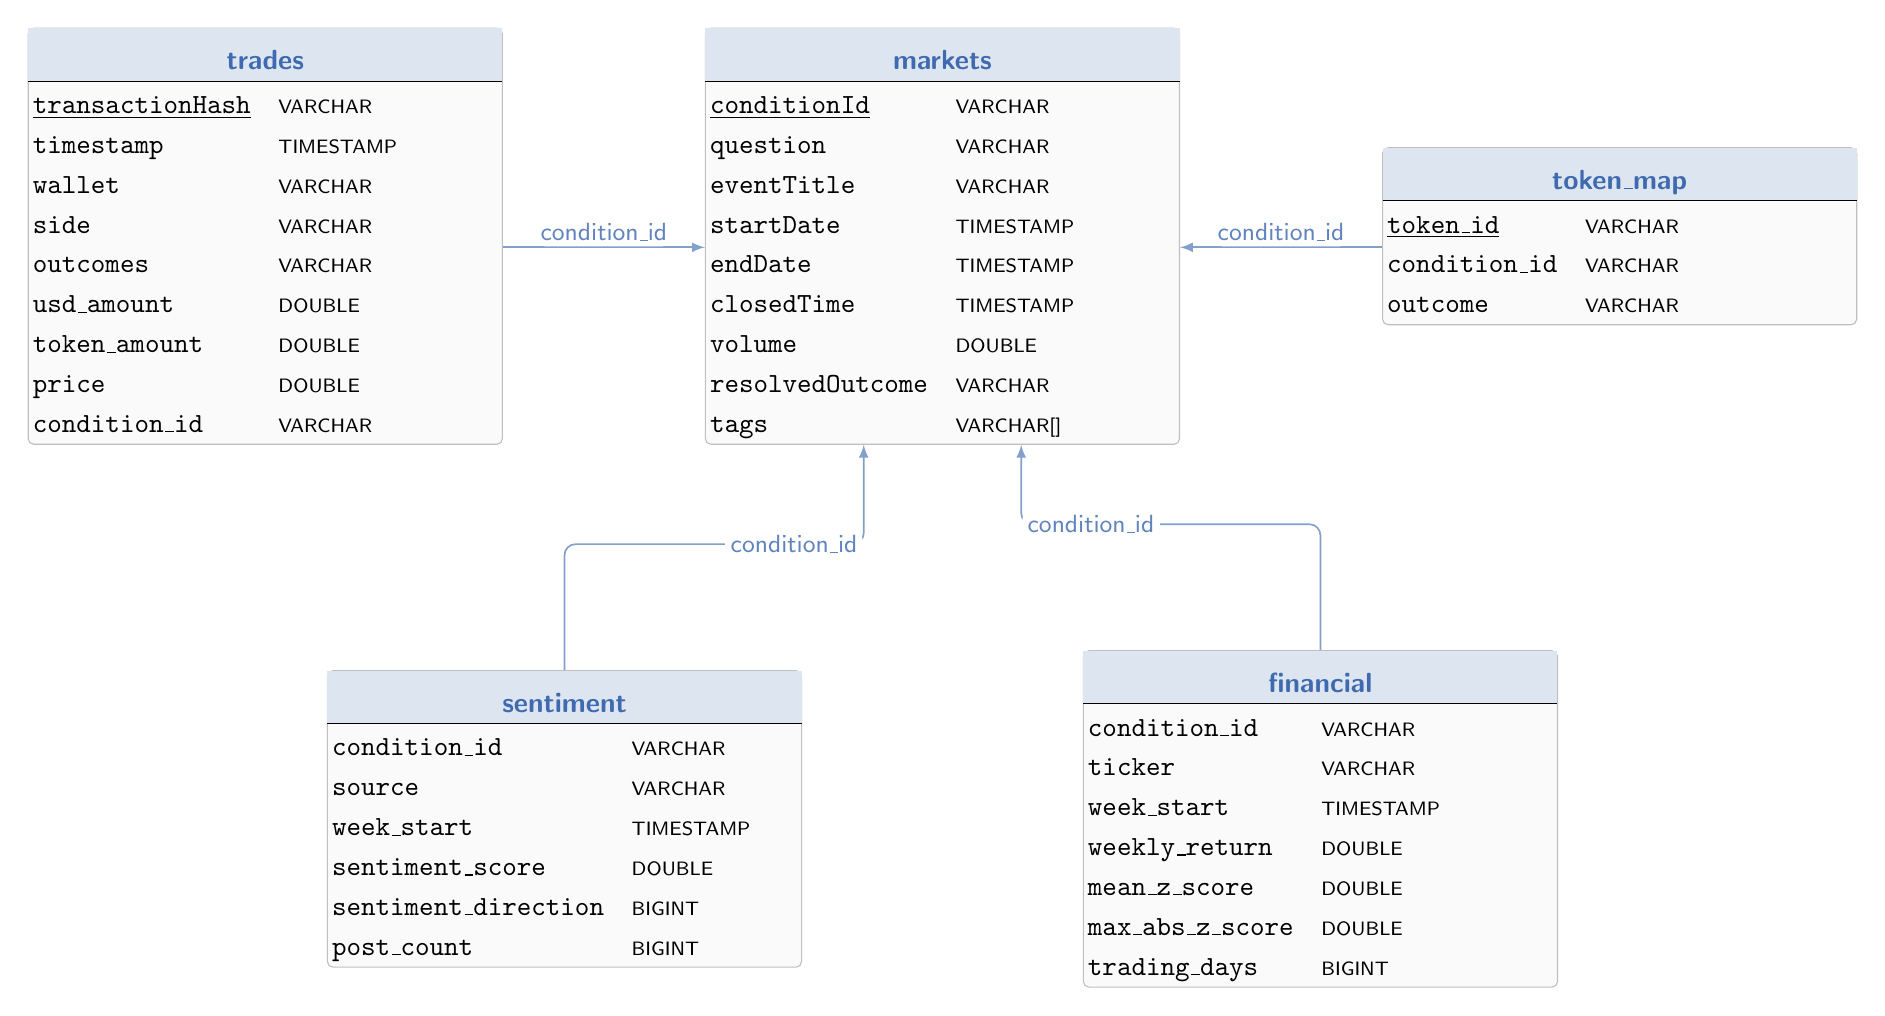
\begin{tikzpicture}[
    fk/.style    = {->, >=latex, semithick, PolyBlue!55},
    fklbl/.style = {font=\small\sffamily, text=PolyBlue!70,
                    fill=white, inner sep=2pt},
]
 
% =====================================================================
%  MARKETS  (top-centre — the hub)
% =====================================================================
\node[draw=gray!50, fill=gray!4, inner sep=0pt, rounded corners=2pt]
    (markets) at (0, 0) {%
    \begin{tabular}{@{\,}l@{\hskip 10pt}l@{\,}}
      \multicolumn{2}{c}{%
        \cellcolor{PolyBlue!15}%
        \makebox[5.6cm][c]{\rule{0pt}{1.5em}%
          \textsf{\textbf{\textcolor{PolyBlue!85}{markets}}}}}\\[-0.4pt]
      \hline \rule{0pt}{1.15em}%
      \underline{\texttt{conditionId}}     & \textsf{\scriptsize VARCHAR}   \\
      \texttt{question}                    & \textsf{\scriptsize VARCHAR}   \\
      \texttt{eventTitle}                  & \textsf{\scriptsize VARCHAR}   \\
      \texttt{startDate}                   & \textsf{\scriptsize TIMESTAMP} \\
      \texttt{endDate}                     & \textsf{\scriptsize TIMESTAMP} \\
      \texttt{closedTime}                  & \textsf{\scriptsize TIMESTAMP} \\
      \texttt{volume}                      & \textsf{\scriptsize DOUBLE}    \\
      \texttt{resolvedOutcome}             & \textsf{\scriptsize VARCHAR}   \\
      \texttt{tags}                        & \textsf{\scriptsize VARCHAR[]} \\
    \end{tabular}%
};
 
% =====================================================================
%  TRADES  (left of markets)
% =====================================================================
\node[draw=gray!50, fill=gray!4, inner sep=0pt, rounded corners=2pt]
    (trades) at (-8.6, 0) {%
    \begin{tabular}{@{\,}l@{\hskip 10pt}l@{\,}}
      \multicolumn{2}{c}{%
        \cellcolor{PolyBlue!15}%
        \makebox[5.6cm][c]{\rule{0pt}{1.5em}%
          \textsf{\textbf{\textcolor{PolyBlue!85}{trades}}}}}\\[-0.4pt]
      \hline \rule{0pt}{1.15em}%
      \underline{\texttt{transactionHash}} & \textsf{\scriptsize VARCHAR}   \\
      \texttt{timestamp}                   & \textsf{\scriptsize TIMESTAMP} \\
      \texttt{wallet}                      & \textsf{\scriptsize VARCHAR}   \\
      \texttt{side}                        & \textsf{\scriptsize VARCHAR}   \\
      \texttt{outcomes}                    & \textsf{\scriptsize VARCHAR}   \\
      \texttt{usd\_amount}                 & \textsf{\scriptsize DOUBLE}    \\
      \texttt{token\_amount}               & \textsf{\scriptsize DOUBLE}    \\
      \texttt{price}                       & \textsf{\scriptsize DOUBLE}    \\
      \textbf{\texttt{condition\_id}}      & \textsf{\scriptsize VARCHAR}   \\
    \end{tabular}%
};
 
% =====================================================================
%  TOKEN_MAP  (right of markets)
% =====================================================================
\node[draw=gray!50, fill=gray!4, inner sep=0pt, rounded corners=2pt]
    (tokenmap) at (8.6, 0) {%
    \begin{tabular}{@{\,}l@{\hskip 10pt}l@{\,}}
      \multicolumn{2}{c}{%
        \cellcolor{PolyBlue!15}%
        \makebox[5.6cm][c]{\rule{0pt}{1.5em}%
          \textsf{\textbf{\textcolor{PolyBlue!85}{token\_map}}}}}\\[-0.4pt]
      \hline \rule{0pt}{1.15em}%
      \underline{\texttt{token\_id}}       & \textsf{\scriptsize VARCHAR} \\
      \textbf{\texttt{condition\_id}}      & \textsf{\scriptsize VARCHAR} \\
      \texttt{outcome}                     & \textsf{\scriptsize VARCHAR} \\
    \end{tabular}%
};
 
% =====================================================================
%  SENTIMENT  (bottom-left)
% =====================================================================
\node[draw=gray!50, fill=gray!4, inner sep=0pt, rounded corners=2pt]
    (sentiment) at (-4.8, -7.4) {%
    \begin{tabular}{@{\,}l@{\hskip 10pt}l@{\,}}
      \multicolumn{2}{c}{%
        \cellcolor{PolyBlue!15}%
        \makebox[5.6cm][c]{\rule{0pt}{1.5em}%
          \textsf{\textbf{\textcolor{PolyBlue!85}{sentiment}}}}}\\[-0.4pt]
      \hline \rule{0pt}{1.15em}%
      \textbf{\texttt{condition\_id}}      & \textsf{\scriptsize VARCHAR}   \\
      \texttt{source}                      & \textsf{\scriptsize VARCHAR}   \\
      \texttt{week\_start}                 & \textsf{\scriptsize TIMESTAMP} \\
      \texttt{sentiment\_score}            & \textsf{\scriptsize DOUBLE}    \\
      \texttt{sentiment\_direction}        & \textsf{\scriptsize BIGINT}    \\
      \texttt{post\_count}                 & \textsf{\scriptsize BIGINT}    \\
    \end{tabular}%
};
 
% =====================================================================
%  FINANCIAL  (bottom-right)
% =====================================================================
\node[draw=gray!50, fill=gray!4, inner sep=0pt, rounded corners=2pt]
    (financial) at (4.8, -7.4) {%
    \begin{tabular}{@{\,}l@{\hskip 10pt}l@{\,}}
      \multicolumn{2}{c}{%
        \cellcolor{PolyBlue!15}%
        \makebox[5.6cm][c]{\rule{0pt}{1.5em}%
          \textsf{\textbf{\textcolor{PolyBlue!85}{financial}}}}}\\[-0.4pt]
      \hline \rule{0pt}{1.15em}%
      \textbf{\texttt{condition\_id}}      & \textsf{\scriptsize VARCHAR}   \\
      \texttt{ticker}                      & \textsf{\scriptsize VARCHAR}   \\
      \texttt{week\_start}                 & \textsf{\scriptsize TIMESTAMP} \\
      \texttt{weekly\_return}              & \textsf{\scriptsize DOUBLE}    \\
      \texttt{mean\_z\_score}              & \textsf{\scriptsize DOUBLE}    \\
      \texttt{max\_abs\_z\_score}          & \textsf{\scriptsize DOUBLE}    \\
      \texttt{trading\_days}               & \textsf{\scriptsize BIGINT}    \\
    \end{tabular}%
};
 
% =====================================================================
%  FK ARROWS — all point inward to markets.conditionId
% =====================================================================
 
% trades.condition_id → markets.conditionId
\draw[fk, rounded corners=4pt]
    ([yshift=-4pt]trades.east) -- ([yshift=-4pt]markets.west)
    node[fklbl, midway, above] {condition\_id};
 
% token_map.condition_id → markets.conditionId
\draw[fk, rounded corners=4pt]
    ([yshift=-4pt]tokenmap.west) -- ([yshift=-4pt]markets.east)
    node[fklbl, midway, above] {condition\_id};
 
% sentiment.condition_id → markets.conditionId
\draw[fk, rounded corners=4pt]
    (sentiment.north) -- ++(0, 1.6)
    -| ([xshift=-1.0cm]markets.south)
    node[fklbl, pos=0.50, left] {condition\_id};
 
% financial.condition_id → markets.conditionId
\draw[fk, rounded corners=4pt]
    (financial.north) -- ++(0, 1.6)
    -| ([xshift=1.0cm]markets.south)
    node[fklbl, pos=0.50, right] {condition\_id};
 
\end{tikzpicture}%



\caption{Database schema.  Underlined fields denote primary keys;
         bold fields are foreign keys referencing
         \texttt{markets.conditionId}.  The \texttt{sentiment} and
         \texttt{financial} tables are populated by the sentiment
         pipeline (Section~\ref{sec:sentiment}).}
\label{fig:schema}
\end{figure}

\noindent An exploratory analysis of the resulting dataset, covering
wallet activity distributions, volume concentration, hit rates, and
market coverage-is provided in Section \ref{sec:eda}.



\newpage

\newpage
% ==========================================================
%  SECTION 3 - SENTIMENT AND FINANCIAL SIGNAL PIPELINE
% ==========================================================
% ==========================================================
%  SECTION 3 - SENTIMENT AND FINANCIAL SIGNAL PIPELINE
% ==========================================================
\section{Sentiment and Financial Signal Pipeline}
\label{sec:sentiment}

The trade data from Section~\ref{sec:pipeline} records wallet
activity but not the external information available at the time of
each trade. This section describes the pipeline that collects three
external signal sources, aggregates each to weekly resolution, and
keys them on \texttt{condition\_id} + \texttt{week\_start} so they
can be joined to trades by market and week:



\begin{itemize}
    \item Financial Times articles (ProQuest exports), scored with
          FinBERT \cite{araci2019finbert}.
    \item Donald Trump's Truth Social posts (29,410 posts from
          \texttt{stiles/trump-truth-social-archive}
          \cite{trump_archive}), scored with VADER
          \cite{hutto2014vader}.
    \item yfinance daily OHLCV for geopolitically-linked tickers,
          converted to weekly abnormal returns against a 20-day
          rolling baseline, with CBOE VIX as a volatility benchmark.
\end{itemize}



% ── 3.1 Architecture Overview ────────────────────────────────────────────────
\subsection{Architecture Overview}
\label{sec:sentiment_architecture}

Figure~\ref{fig:sentiment_pipeline} shows the three parallel tracks
that produce the enrichment tables. All three consume the shared
\texttt{markets} table and NER module, and all three write into the
same \texttt{polymarket.ddb} database established in
Section~\ref{sec:pipeline}. A single vocabulary module,
\texttt{pipeline\_config.py}, drives keyword-to-corpus, keyword-to-ticker,
and author-stopword mappings across all three collectors — covered
in the subsections that follow.

\begin{figure}[H]
\centering
\resizebox{\textwidth}{!}{%
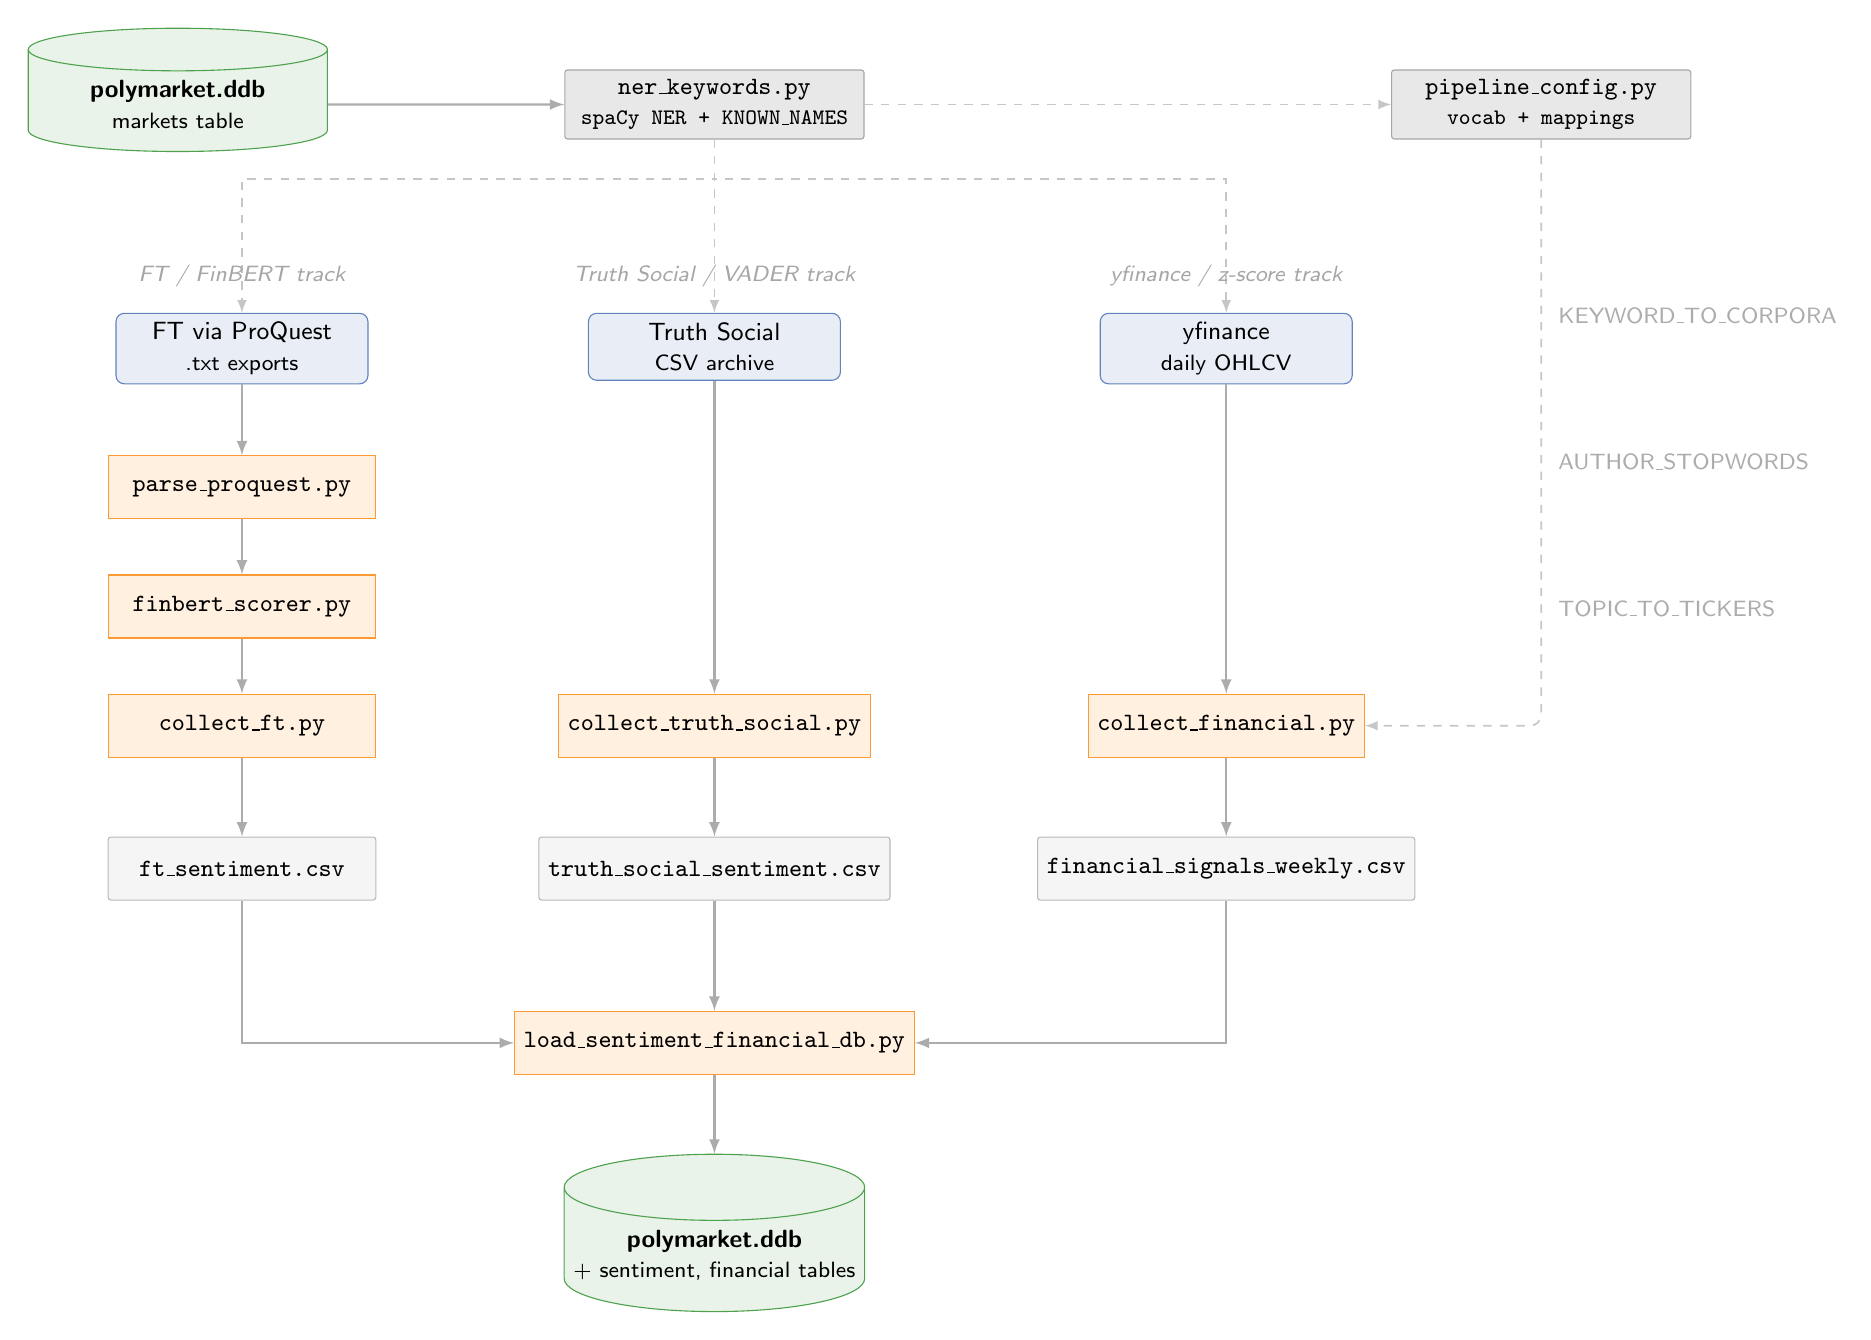
\begin{tikzpicture}[
    node distance = 0.7cm and 1.5cm,
    % ── Node styles (match Figure 1) ──
    api/.style   = {rectangle, rounded corners=3pt,
                    draw=PolyBlue!70, fill=PolyBlue!10,
                    minimum width=3.2cm, minimum height=0.85cm,
                    font=\small\sffamily, align=center},
    script/.style= {rectangle,
                    draw=orange!80, fill=orange!12,
                    minimum width=3.4cm, minimum height=0.8cm,
                    font=\small\ttfamily, align=center},
    file/.style  = {rectangle, rounded corners=1pt,
                    draw=gray!55, fill=gray!8,
                    minimum width=3.4cm, minimum height=0.8cm,
                    font=\small\ttfamily, align=center},
    shared/.style= {rectangle, rounded corners=1pt,
                    draw=gray!70, fill=gray!18,
                    minimum width=3.8cm, minimum height=0.85cm,
                    font=\small\ttfamily\bfseries, align=center},
    db/.style    = {cylinder, shape border rotate=90, aspect=0.22,
                    draw=ForestGreen!80, fill=ForestGreen!10,
                    minimum width=3.8cm, minimum height=1.1cm,
                    font=\small\sffamily\bfseries, align=center},
    arr/.style   = {->, >=latex, thick, gray!65},
    dep/.style   = {->, >=latex, semithick, gray!45, dashed},
    labl/.style  = {font=\footnotesize\sffamily\itshape, text=gray!70},
    deplbl/.style= {font=\footnotesize\sffamily, text=gray!65,
                    fill=white, inner sep=2pt},
]

% =====================================================================
%  ROW 0 : shared inputs
% =====================================================================
\node[db] (markets) at (0,0) {polymarket.ddb\\
    {\footnotesize\mdseries markets table}};

\node[shared, right=3.0cm of markets] (ner)
    {ner\_keywords.py\\
    {\footnotesize\mdseries spaCy NER + KNOWN\_NAMES}};

% pipeline_config now sits directly above where collect_financial.py will be
% fin_src is at xshift=6.5cm of ner (row 1), so match that x position
\node[shared] (config) at ($(ner) + (10.5cm, 0)$)
    {pipeline\_config.py\\
    {\footnotesize\mdseries vocab + mappings}};

\draw[arr] (markets) -- (ner);

% NER depends on pipeline_config
\draw[dep] (ner) -- (config);

% =====================================================================
%  ROW 1 : external sources
% =====================================================================
\node[api, below=2.2cm of ner, xshift=-6.0cm] (ft_src)
    {FT via ProQuest\\{\footnotesize .txt exports}};
\node[api, below=2.2cm of ner]                 (ts_src)
    {Truth Social\\{\footnotesize CSV archive}};
\node[api, below=2.2cm of ner, xshift=6.5cm]   (fin_src)
    {yfinance\\{\footnotesize daily OHLCV}};

% NER drives keyword extraction in all three tracks
\draw[dep] (ner.south) -- ++(0,-0.5) -| (ft_src.north);
\draw[dep] (ner.south) -- (ts_src.north);
\draw[dep] (ner.south) -- ++(0,-0.5) -| (fin_src.north);

% =====================================================================
%  ROW 2 : FT-only intermediate scripts
% =====================================================================
\node[script, below=0.9cm of ft_src] (parse)
    {parse\_proquest.py};
\node[script, below=0.7cm of parse]  (finbert)
    {finbert\_scorer.py};

\draw[arr] (ft_src) -- (parse);
\draw[arr] (parse)  -- (finbert);

% =====================================================================
%  ROW 3 : collectors — aligned on one row
% =====================================================================
\node[script, below=0.7cm of finbert] (ft_col)
    {collect\_ft.py};
\node[script] (ts_col) at (ts_src |- ft_col)
    {collect\_truth\_social.py};
\node[script] (fin_col) at (fin_src |- ft_col)
    {collect\_financial.py};

\draw[arr] (finbert) -- (ft_col);
\draw[arr] (ts_src)  -- (ts_col);
\draw[arr] (fin_src) -- (fin_col);

% =====================================================================
%  pipeline_config.py → collect_financial.py
%  Drop straight down from config, then turn left into fin_col.east
% =====================================================================
\coordinate (cfg-bottom) at (config.south |- fin_col.east);

\draw[dep, rounded corners=4pt]
    (config.south) -- (cfg-bottom) -- (fin_col.east);

% stacked labels on the vertical segment, to the right of the line
\node[deplbl, right=4pt] at ($(config.south)!0.30!(cfg-bottom)$)
    {KEYWORD\_TO\_CORPORA};
\node[deplbl, right=4pt] at ($(config.south)!0.55!(cfg-bottom)$)
    {AUTHOR\_STOPWORDS};
\node[deplbl, right=4pt] at ($(config.south)!0.80!(cfg-bottom)$)
    {TOPIC\_TO\_TICKERS};

% =====================================================================
%  ROW 4 : output CSVs — aligned
% =====================================================================
\node[file, below=1.0cm of ft_col]  (ft_csv)
    {ft\_sentiment.csv};
\node[file] (ts_csv) at (ts_col |- ft_csv)
    {truth\_social\_sentiment.csv};
\node[file] (fin_csv) at (fin_col |- ft_csv)
    {financial\_signals\_weekly.csv};

\draw[arr] (ft_col)  -- (ft_csv);
\draw[arr] (ts_col)  -- (ts_csv);
\draw[arr] (fin_col) -- (fin_csv);

% =====================================================================
%  ROW 5 : loader + destination DB
% =====================================================================
\node[script, below=1.4cm of ts_csv] (loader)
    {load\_sentiment\_financial\_db.py};

\draw[arr] (ft_csv.south)  |- (loader.west);
\draw[arr] (ts_csv.south)  -- (loader.north);
\draw[arr] (fin_csv.south) |- (loader.east);

\node[db, below=1.0cm of loader] (ddb)
    {polymarket.ddb\\
    {\footnotesize\mdseries + sentiment, financial tables}};

\draw[arr] (loader.south) -- (ddb.north);

% =====================================================================
%  column labels
% =====================================================================
\node[labl, above=0.2cm of ft_src]  {FT / FinBERT track};
\node[labl, above=0.2cm of ts_src]  {Truth Social / VADER track};
\node[labl, above=0.2cm of fin_src] {yfinance / z-score track};

\end{tikzpicture}
}% end resizebox
\caption{Sentiment and financial enrichment pipeline. Orange: Python
         scripts, blue: external data sources, grey: intermediate
         files and shared resources, green: DuckDB. Solid arrows:
         primary data flow; dashed arrows: vocabulary and
         configuration dependencies.}

\label{fig:sentiment_pipeline}
\end{figure}

\noindent spaCy's default NER is not sufficient on its own for this
domain. Market questions present three specific challenges:

\begin{itemize}
    \item \textbf{Short and fragmented:} Questions are typically
          under 15 words and often start with proper nouns,
          confusing \texttt{spaCy}'s sentence parser.
    \item \textbf{Out-of-vocabulary entities:} Names outside \texttt{spaCy's}
          default English model include frontline town names
          (\texttt{Pokrovsk}, \texttt{Sudzha}, \texttt{Siversk},
          \texttt{Kupiansk}), faction names (\texttt{Houthi},
          \texttt{HTS}, \texttt{PKK}), and transliterated leaders
          (\texttt{Al-Sharaa}, \texttt{Khamenei}).
    \item \textbf{Surface-form variation:} The same entity appears
          in multiple forms such as \texttt{Benjamin Netanyahu},
          \texttt{Netanyahu}, \texttt{Israel's PM}, \texttt{Bibi Netanyahu}. Which all need to be collapsed to a single canonical name.
\end{itemize}

\noindent \texttt{ner\_keywords.py} handles these with a three-pass
design backed by a shared vocabulary.

\subsubsection*{Three-Pass Extraction}

The extractor loads spaCy's \texttt{en\_core\_web\_sm} model and
runs three passes over each question, each covering a failure mode
of the previous one:

\begin{enumerate}
    \item \textbf{spaCy NER:} Extract entities of type \texttt{GPE},
          \texttt{PERSON}, \texttt{ORG}, or \texttt{NORP} and
          normalises it through the \texttt{KNOWN\_NAMES}. Before parsing, a
          neutral prefix \texttt{"About: "} is taken from the
          question so that sentence-initial proper nouns
          (\texttt{"Xi Jinping out in 2025?"}) are not misread as
          verbs.
    \item \textbf{Proper noun fallback:} Any word tagged as a proper
      noun that Pass 1 missed is added and normalised. Catches
      names spaCy recognised as a name but did not classify.

    \item \textbf{\texttt{KNOWN\_NAMES} phrase lookup:} The remaining
        tokens are checked against \texttt{KNOWN\_NAMES} in phrases
        of decreasing length. Checks three words first, then two, then one, so that multi-word names like \texttt{"Gulf Leaders Summit"}
        are matched as a single unit rather than split into separate
        keywords. This ultimately catches names spaCy does not recognise at all.
\end{enumerate}

\lstdefinestyle{mystyle}{
    basicstyle=\small\ttfamily,
    breaklines=true,
    keywordstyle=\color{blue},
    commentstyle=\color{green!50!black},
    stringstyle=\color{red!70!black},
    showstringspaces=false,
    tabsize=4,
}
\lstset{style=mystyle}

\caption{Pass 3: sliding phrase lookup in \texttt{KNOWN\_NAMES}.}
\label{lst:phrase_lookup}
\end{listing}
\newpage
\noindent Figure~\ref{fig:ner_flow} walks through a worked example
and shows where each pass contributes.


\begin{figure}[H]
\centering
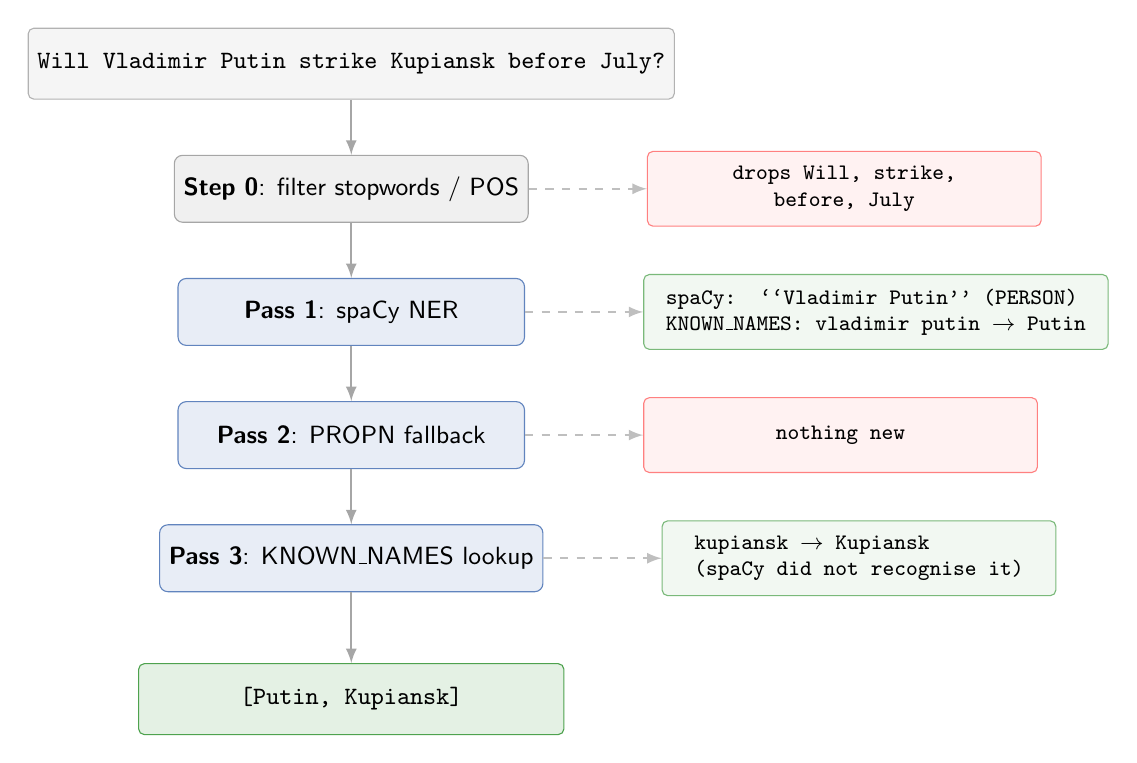
\begin{tikzpicture}[
    qbox/.style   = {rectangle, rounded corners=2pt,
                     draw=gray!60, fill=gray!8,
                     minimum width=6.8cm, minimum height=0.9cm,
                     font=\small\ttfamily, align=center},
    filter/.style = {rectangle, rounded corners=3pt,
                     draw=gray!70, fill=gray!12,
                     minimum width=4.4cm, minimum height=0.85cm,
                     font=\small\sffamily, align=center},
    stage/.style  = {rectangle, rounded corners=3pt,
                     draw=PolyBlue!70, fill=PolyBlue!10,
                     minimum width=4.4cm, minimum height=0.85cm,
                     font=\small\sffamily, align=center},
    drop/.style   = {rectangle, rounded corners=2pt,
                     draw=red!50, fill=red!5,
                     minimum width=5.0cm, minimum height=0.95cm,
                     font=\footnotesize\ttfamily, align=center},
    keep/.style   = {rectangle, rounded corners=2pt,
                     draw=ForestGreen!60, fill=ForestGreen!6,
                     minimum width=5.0cm, minimum height=0.95cm,
                     font=\footnotesize\ttfamily, align=left,
                     inner xsep=8pt},
    result/.style = {rectangle, rounded corners=2pt,
                     draw=ForestGreen!80, fill=ForestGreen!12,
                     minimum width=5.4cm, minimum height=0.9cm,
                     font=\small\ttfamily\bfseries, align=center},
    arr/.style    = {->, >=latex, thick, gray!70},
]

% ─── Input question ──────────────────────────────────────────────────────
\node[qbox] (q)
    {Will Vladimir Putin strike Kupiansk before July?};

% ─── Step 0: stopword / POS filter ───────────────────────────────────────
\node[filter, below=0.7cm of q] (f)
    {\textbf{Step 0}: filter stopwords / POS};
\draw[arr] (q) -- (f);

\node[drop, right=1.5cm of f] (f_drop)
    {drops \texttt{Will}, \texttt{strike},\\
     \texttt{before}, \texttt{July}};
\draw[arr, gray!50, dashed] (f.east) -- (f_drop.west);

% ─── Pass 1: spaCy NER ───────────────────────────────────────────────────
\node[stage, below=0.7cm of f] (p1)
    {\textbf{Pass 1}: spaCy NER};
\draw[arr] (f) -- (p1);

\node[keep, right=1.5cm of p1] (p1_keep)
    {spaCy: ``Vladimir Putin'' (PERSON)\\
     \texttt{KNOWN\_NAMES}: \texttt{vladimir putin} $\rightarrow$ \texttt{Putin}};
\draw[arr, gray!50, dashed] (p1.east) -- (p1_keep.west);

% ─── Pass 2: proper noun fallback ────────────────────────────────────────
\node[stage, below=0.7cm of p1] (p2)
    {\textbf{Pass 2}: PROPN fallback};
\draw[arr] (p1) -- (p2);

\node[drop, right=1.5cm of p2] (p2_drop)
    {nothing new};
\draw[arr, gray!50, dashed] (p2.east) -- (p2_drop.west);

% ─── Pass 3: KNOWN_NAMES phrase lookup ───────────────────────────────────
\node[stage, below=0.7cm of p2] (p3)
    {\textbf{Pass 3}: KNOWN\_NAMES lookup};
\draw[arr] (p2) -- (p3);

\node[keep, right=1.5cm of p3] (p3_keep)
    {\texttt{kupiansk} $\rightarrow$ \texttt{Kupiansk}\\
     (spaCy did not recognise it)};
\draw[arr, gray!50, dashed] (p3.east) -- (p3_keep.west);

% Output
\node[result, below=0.9cm of p3] (out)
    {[Putin, Kupiansk]};1
\draw[arr] (p3) -- (out);

\end{tikzpicture}
\caption{Worked example of the three-pass extractor on the question
         \texttt{"Will Vladimir Putin strike Kupiansk before July?"}.
         Step 0 drops stopwords. Pass 1 captures
         \texttt{"Vladimir Putin"} via spaCy NER, which
         \texttt{KNOWN\_NAMES} then normalises to \texttt{Putin}.
         Pass 2 adds nothing. Pass 3 rescues \texttt{Kupiansk}, a
         Ukrainian frontline town that spaCy does not recognise.}
\label{fig:ner_flow}
\end{figure}


\subsubsection*{Vocabulary}

Two dictionaries in \texttt{pipeline\_config.py} control the output
of all three passes. Tables~\ref{tab:stopwords}
and~\ref{tab:known_names} summarise what each does.

\begin{table}[H]
\centering
\caption{\texttt{STOPWORDS} categories (approx.\ 120 entries total).}
\label{tab:stopwords}
\small
\begin{tabularx}{\textwidth}{l X}
\toprule
\textbf{Category} & \textbf{Examples} \\
\midrule
Market boilerplate & \texttt{yes}, \texttt{no}, \texttt{will},
                     \texttt{resolve}, \texttt{market}, \texttt{date} \\
Calendar tokens    & months, \texttt{q1}–\texttt{q4},
                     \texttt{2023}–\texttt{2026}, \texttt{first},
                     \texttt{second} \\
Generic titles     & \texttt{president}, \texttt{prime},
                     \texttt{minister}, \texttt{secretary},
                     \texttt{chancellor} \\
NER noise          & \texttt{god}, \texttt{clock}, \texttt{trillion},
                     \texttt{emergency}, \texttt{victory} \\
\bottomrule
\end{tabularx}
\end{table}

\begin{table}[H]
\centering
\caption{\texttt{KNOWN\_NAMES} transformation categories
         (approx.\ 250 entries total).}
\label{tab:known_names}
\small
\begin{tabularx}{\textwidth}{l X}
\toprule
\textbf{Transformation} & \textbf{Example mapping} \\
\midrule
Name variants       & \texttt{benjamin netanyahu} $\rightarrow$ \texttt{Netanyahu} \\
Demonyms            & \texttt{israeli}            $\rightarrow$ \texttt{Israel}    \\
Abbreviations       & \texttt{u.s.}               $\rightarrow$ \texttt{USA}       \\
Multi-word phrases  & \texttt{gulf leaders summit} $\rightarrow$ \texttt{Gulf Leaders Summit} \\
Out-of-vocab names  & \texttt{pokrovsk}           $\rightarrow$ \texttt{Pokrovsk}  \\
Possessive stripping & \texttt{Israel's}          $\rightarrow$ \texttt{Israel}   \\
\bottomrule
\end{tabularx}
\end{table}


\subsubsection*{Coverage}

Running \texttt{ner\_keywords.py} across all 1,801 resolved markets
with trades yields 328 unique keywords, averaging 1.93
per market. The top 10 account for most of the coverage
(Table~\ref{tab:top_keywords}), and a lot of  keywords
covers one or two markets each. The overall sentiment and financial
coverage breakdown, including markets that produce no keywords at
all, is reported in Section~\ref{sec:sentiment_coverage}.

\begin{table}[H]
\centering
\caption{Top 10 keywords by market coverage.}
\label{tab:top_keywords}
\small
\begin{tabularx}{0.6\textwidth}{X r}
\toprule
\textbf{Keyword} & \textbf{Markets} \\
\midrule
Israel    & 412 \\
Trump     & 396 \\
Iran      & 223 \\
USA       & 182 \\
Russia    & 167 \\
Zelenskyy & 116 \\
Ukraine   & 105 \\
Yemen     & 100 \\
Putin     &  98 \\
Gaza      &  67 \\
\bottomrule
\end{tabularx}
\end{table}




% ── 3.3 Financial Times — ProQuest Corpus and FinBERT ──────────────────────
\subsection{Financial Times --- ProQuest Corpus and FinBERT}
\label{sec:ft_finbert}

The Financial Times track produces weekly sentiment scores for each
market from FT coverage during the market's lifetime. This section runs in four stages: Corpus acquisition, parsing, FinBERT scoring, and weekly aggregation.



\subsubsection*{Corpus Acquisition}
\label{sec:corpus_acquisition}

ProQuest does not expose a bulk download API at the UCD subscription
tier --- articles must be selected through the web interface and
exported as \texttt{.txt} files. A market-by-market download is
therefore not feasible. Queries were constructed manually, guided by
the NER keyword distribution in Section~\ref{sec:ner_keywords}, with
three targeting decisions per query.

\paragraph{Query scope.} Bare single-keyword queries for common
terms like \texttt{"Russia"} or \texttt{"Iran"} return tens of
thousands of FT articles and cannot be practically exported. These
were narrowed to two-keyword AND combinations (e.g.\
\texttt{"Russia" AND "Ukraine"}). For niche entities like
\texttt{"Houthi"}, \texttt{"Kupiansk"}, or \texttt{"Milei"}, the
article count is already bounded and single-keyword queries were
used directly.

\paragraph{Date window.} Each query was constrained to the lifetime
of the markets it supports, with a 30-day lead added before the
earliest market opens to capture the immediate pre-opening news
cycle (Table~\ref{tab:date_windows}).

\begin{table}[H]
\centering
\caption{Date windows for three representative topics.}
\label{tab:date_windows}
\small
\begin{tabularx}{\textwidth}{l l l X}
\toprule
\textbf{Topic} & \textbf{Window} & \textbf{Articles} & \textbf{Rationale} \\
\midrule
\texttt{russia\_ukraine}    & 2023-01 -- 2025-10 & 5{,}132
    & Continuous market coverage throughout the war. \\
\addlinespace[3pt]
\texttt{saudi\_arabia\_usa} & 2025-04 -- 2025-10 & 1{,}133
    & Markets opened spring 2025 around the Gulf Leaders Summit. \\
\addlinespace[3pt]
\texttt{elon\_musk\_trump}  & 2024-12 -- 2025-10 & 2{,}040
    & Markets tracked a specific feud window. \\
\bottomrule
\end{tabularx}
\end{table}

\paragraph{Batching.} ProQuest exports are capped at 500 articles
per batch. High-volume topics required many batches:
\texttt{russia\_ukraine} in 53, \texttt{china\_taiwan} in 35, while
niche topics like \texttt{houthi} and \texttt{bolsonaro} required
a single batch. Batch counts do not map linearly to article counts
because some batch sizes are 100 others are 500.

\paragraph{} In total, 72 topic corpora were acquired spanning
1 February 2023 to 31 October 2025. \texttt{parse\_proquest.py}
(Section~\ref{sec:parsing}) produced 63{,}874 parsed articles;
\texttt{finbert\_scorer.py} (Section~\ref{sec:finbert_scoring})
scored 51{,}647. The ${\sim}19\%$ gap consists of broad
single-keyword corpora that were parsed early in development but
later superseded by narrower two-keyword AND queries, and so were
not carried through to scoring. Table~\ref{tab:corpus_sizes} shows
the 10 largest scored corpora.

\begin{table}[H]
\centering
\caption{Top 10 ProQuest corpora by scored article count.}
\label{tab:corpus_sizes}
\small
\begin{tabularx}{\textwidth}{X r r l}
\toprule
\textbf{Topic} & \textbf{Batches} & \textbf{Articles} & \textbf{Date range} \\
\midrule
russia\_ukraine   & 53 & 5{,}132 & 2024-08 -- 2025-10 \\
china\_taiwan     & 35 & 3{,}390 & 2023-12 -- 2025-10 \\
moscow\_ukraine   & 32 & 3{,}132 & 2024-02 -- 2025-10 \\
gaza\_israel      & 28 & 2{,}668 & 2024-05 -- 2025-10 \\
hamas\_israel     & 22 & 2{,}140 & 2024-06 -- 2025-10 \\
iran\_usa         &  5 & 2{,}051 & 2023-11 -- 2025-10 \\
elon\_musk\_trump &  5 & 2{,}040 & 2025-01 -- 2025-10 \\
iran\_israel      &  4 & 1{,}757 & 2024-05 -- 2025-10 \\
trump\_putin      & 19 & 1{,}648 & 2024-11 -- 2025-10 \\
netanyahu         &  3 & 1{,}472 & 2024-09 -- 2025-10 \\
\bottomrule
\end{tabularx}
\end{table}

% =========================================================
\section{Exploratory Wallet Analysis and Feature Motivation}
\label{sec:eda}
% =========================================================

%This section tests the core hypothesis that drives the rest of the report: \emph{potentially informed activity on Polymarket is concentrated in a small subset of wallets that are simultaneously large, accurate, early, and topic-specialised}. 

Each of the four dimensions examined below (volume, hit rate, timing, domain concentration) is turned into a feature family in Section~\ref{sec:ml}: volume and timing feed the trade-context block (\texttt{log\_net\_usd}, \texttt{hours\_before}, \texttt{log\_market\_volume}), hit-rate feeds the wallet-history block, and domain concentration underpins the market-context block. Here we'll set out the feature design of Section~\ref{sec:ml} and the capital-allocation logic of Section~\ref{sec:business}, and to quantify the survivorship/selection bias that justifies the cold-start validation scheme (Table~\ref{tab:test_train_struct}).

\paragraph{Definitions used throughout this section.}
\begin{itemize}[label=--, leftmargin=1.5em, itemsep=1pt]
    \item \texttt{hit\_rate}~$=$~$\frac{\texttt{markets\_correct}}{\texttt{markets\_traded}}$, where for each (wallet, market) pair the bet is the outcome token on which the wallet has the largest positive net-USD position (multi-outcome markets handled via \texttt{ROW\_NUMBER() OVER (PARTITION BY)}). We excluded positions with \texttt{net\_usd}~$=0$).
    \item \texttt{realised\_edge}~$=$~\texttt{outcome\_correct}~$-$~\texttt{avg\_price}, the same economic score used in Section~\ref{sec:ml} (Table~\ref{tab:score_stack}). Computing this at wallet level is what lets the EDA feed directly into the ML target rather than being a parallel descriptive exercise.
    \item \texttt{whale\_quadrant}~$=\{$\texttt{hit\_rate}~$\geq 65\%$ \textbf{and} \texttt{total\_volume}~$\geq Q_{75}\}$, where $Q_{75}\approx\$\WhaleVolQSeventyFive$ is the 75th percentile of volume among experienced wallets.
    \item \texttt{early\_wallet}~$=\{\mathbb{E}[\texttt{days\_before\_resolution}] \geq \EarlyThresholdDays\}$, the 75th percentile of per-wallet average BUY-side days-before-resolution (using \texttt{COALESCE(closedTime, endDate)} as the resolution timestamp; SELL trades and markets without a close timestamp are excluded).
    \item \texttt{experienced} wallets are those with $\geq 10$ resolved markets.
     %This is a survivorship filter and its sensitivity is reported in Table~\ref{tab:eda_threshold_sens}.
\end{itemize}

All inferential statements in this section use wallet-clustered bootstrap (3{,}000 iterations) rather than row-level standard errors, matching the inference techniques used in Figure~\ref{fig:bootstrap}.

\subsection{Data funnel from raw trades to modelling sample}
\label{sec:eda_funnel}

Before describing the wallet-level EDA it is useful to state the full data funnel, because the three universes used in this report (raw trade universe, EDA wallet universe, modelling-observation universe) are distinct, so we'll briefly give some context on this:

\begin{table}[H]
\centering
\small
\setlength{\tabcolsep}{8pt}
\begin{adjustbox}{max width=0.95\textwidth}
\begin{tabular}{lrl}
\toprule
Stage & Rows & Row definition \\
\midrule
Raw trades (post-dedup)                 & 5{,}932{,}723 & One fill per row (after removing 567{,}477 duplicates) \\
EDA wallet universe                     & \RawUniqueWallets & One row per wallet \\
\quad of which experienced ($\geq 10$ markets) & \ExpWallets\ (\ExpWalletsPct\%) & Used for hit-rate / whale-quadrant analysis \\
Modelling observations (Section~\ref{sec:ml}) & 394{,}279 & One row per (wallet, market) buy-side position \\
\quad of which diagnostic informed labels & \PositiveLabels\ (0.2\%) & \edit{\texttt{informed\_label}~$=1$; used only for feature engineering diagnostics, not as the final ML target} \\
\bottomrule
\end{tabular}
\end{adjustbox}
\caption{Data funnel: three universes used in the report, each with its own row definition.}
\label{tab:data_funnel}
\end{table}

External text coverage on the modelling sample is uneven: Truth Social weekly coverage is 100.0\%, market-specific Truth Social coverage is 25.6\%, and FT coverage is 56.7\%. Thus, ML model in Section~\ref{sec:ml} can't lean on sentiment alone and must combine wallet history, market context, and partial sentiment coverage. \edit{That} is why our evaluation uses feature-family ablation in Table~\ref{tab:ml_main_results}.

\subsection{Wallet activity and volume concentration}

The wallet data shows a highly skewed market structure. There are \RawUniqueWallets\ unique wallets, but activity is concentrated in a small minority. The median wallet makes just \MedTradesPerWallet\ trades, rising to 14 at the 75th percentile and 316 at the 99th percentile. Volume concentration is even more extreme: the top 50 wallets account for \TopfVolumeShare\% of total volume, and only \WalletsHalfVolume\ wallets generate 50\% of all volume. This skew is the empirical basis for the capital-allocation logic in Section~\ref{sec:business}: a ranking model is useful precisely because trade-level edge is concentrated in a small tail.


%A manual review of the largest addresses in the sample identified two official Polymarket exchange contract addresses rather than ordinary trader wallets:
%
%\begin{itemize}
%    \item \texttt{0x4bfb41d5b3570defd03c39a9a4d8de6bd8b8982e} -- CTF Exchange
%    \item \texttt{0xc5d563a36ae78145c45a50134d48a1215220f80a} -- Neg Risk CTF Exchange
%\end{itemize}
%
%These contract addresses are \textbf{excluded from the modelling table used in Section~\ref{sec:ml}} and from the whale-quadrant, early-wallet, and smart-wallet exports (see \texttt{wallet\_Analysis\_v2.ipynb}, Cell~2.3). They are retained only in the descriptive raw-activity table below (Table~\ref{tab:top10_wallets_trade_count}) to document their scale. Other non-publicly identified market-making or infrastructure wallets may still be present in the dataset, so rankings involving the very largest addresses should be interpreted with caution (Polymarket, no date).

\vspace{-1.25em}
\begin{figure}[H]
    \centering
    
\includegraphics[width=0.45\textwidth]{figures/wallet_activity.png}
    
\includegraphics[width=0.45\textwidth]{figures/cum_volume_curve.png}
    \caption{Left: Wallet activity distribution (log scale), Right: Cumulative percentage of total volume by wallet rank.}
    \label{fig:wallet_activity_distribution}
\end{figure}

%\vspace{-1.25em}
%\begin{figure}[H]
%    \centering
%    
\includegraphics[width=0.5\textwidth]{cum_volume_curve.png}
%    \caption{Cumulative percentage of total volume by wallet rank.}
%    \label{fig:volume_concentration_curve}
%\end{figure}

\begin{table}[H]
\centering
\scriptsize
\setlength{\tabcolsep}{4pt}
\begin{adjustbox}{max width=\textwidth}
\begin{tabular}{lrrrr}
\toprule
Wallet & Trade Count & Markets Traded & Total Volume & Last Trade \\
\midrule
0x4bfb41d5b3570defd03c39a9a4d8de6bd8b8982e & \edit{2,147,253} & \edit{1,591} & \edit{481,476,957} & 2025-10-07 16:39:46 \\
0xc5d563a36ae78145c45a50134d48a1215220f80a & 317,028 & 213 & 20,364,754 & 2025-10-07 16:38:54 \\
0xf0b0ef1d6320c6be896b4c9c54dd74407e7f8cab & \edit{169,614} & \edit{1,306} & \edit{3,606,300} & 2025-10-07 16:38:54 \\
0x3078db4a9737866b4d6529f655025b3a20f80389 & \edit{89,643} & \edit{396} & \edit{520,978} & 2025-10-07 08:16:40 \\
0x1cfc260bfa2b5ae89377863180ca3b4f5c862111 & \edit{61,056} & \edit{1,135} & \edit{4,192,330} & 2025-10-07 16:39:46 \\
0x21ffd2b7a212a6f277ed3eca1a9f8efcbca90d71 & \edit{60,357} & \edit{807} & \edit{2,310,365} & 2025-10-07 16:22:36 \\
0xc8ab97a9089a9ff7e6ef0688e6e591a066946418 & \edit{58,203} & \edit{1,212} & \edit{9,644,808} & 2025-10-07 16:38:20 \\
0x7c3db723f1d4d8cb9c550095203b686cb11e5c6b & \edit{57,175} & \edit{658} & \edit{27,555,375} & 2025-10-07 16:39:46 \\
0xd218e474776403a330142299f7796e8ba32eb5c9 & 55,886 & 189 & 2,762,608 & 2025-10-07 16:38:50 \\
0xe6c9eee27de792a9fdcdd322822452625d0f975e & 44,828 & 206 & 673,733 & 2025-10-07 16:29:56 \\
\bottomrule
\end{tabular}
\end{adjustbox}
\caption{Top 10 wallets by trade count}
\label{tab:top10_wallets_trade_count}
\end{table}
\subsection{Hit rate distribution and threshold sensitivity}

Hit rate is computed on resolved markets only, using the multi-outcome-aware net-long rule defined above. The main analysis focuses on experienced wallets ($\geq 10$ resolved markets) to suppress small-sample noise. This leaves \ExpWallets\ wallets, or \ExpWalletsPct\% of total wallets. Within this group, the median hit rate is \ExpMedianHit\% (bootstrap 95\% CI \MedianHitCI), above a 50\% benchmark, while the 75th percentile reaches \ExpPsfHit\%. In total, \ExpWalletsAboveSixtyFive\ wallets achieve a hit rate of at least 65\%.

Because the $\geq 10$-market cutoff, the 65\% hit-rate threshold, and the top-25\% volume cutoff are all analyst-chosen, we report their sensitivity explicitly in Table~\ref{tab:eda_threshold_sens} rather than leaving them as ex post decisions. The shape of the distribution is not threshold-fragile: the qualitative conclusion -- that a material subset of wallets outperforms the 50\% baseline in a way that persists across volume tiers -- holds at $\{5,10,20\}$-market cutoffs and $\{55\%,60\%,65\%\}$ hit-rate thresholds.

\begin{table}[H]
\centering
\small
\begin{tabular}{lrrr}
\toprule
Min resolved markets & Surviving wallets & Median hit rate (\%) & Whale-quadrant @ 65\% \& $Q_{75}$ vol \\
\midrule
5   & \ExpWalletsAtFive     & \MedianHitAtFive   & --   \\
10 (primary) & \ExpWallets  & \ExpMedianHit      & \WhaleQuadrantCount \\
20  & \ExpWalletsAtTwenty   & \MedianHitAtTwenty & --   \\
\bottomrule
\end{tabular}
\caption{Sensitivity of the experienced-wallet universe and the whale-quadrant count to the two analyst-chosen thresholds. Numbers are point estimates; wallet-clustered 95\% CIs available in the notebook.}
\label{tab:eda_threshold_sens}
\end{table}


\begin{figure}[H]
    \centering
    
\includegraphics[width=\textwidth]{figures/hitrate.png}
    
    \vspace{-1em}
    \caption{Hit rate distribution for wallets with at least 10 resolved markets.}
    \label{fig:hit_rate_distribution}
\end{figure}


\begin{table}[H]
\centering

\scriptsize
\setlength{\tabcolsep}{4pt}
\begin{adjustbox}{max width=\textwidth}
\begin{tabular}{lrrrrrr}
\toprule
Wallet & Markets Traded & Markets Correct & Hit Rate (\%) & Total Volume (\$) & Total Trades & Avg Volume per Market (\$) \\
\midrule
% CTF Exchange contract address 0x4bfb41...982e removed — see Section 1.2 disclosure and notebook Cell 2.3.
0x44c1dfe43260c94ed4f1d00de2e1f80fb113ebc1 & 165 & 123 & 74.55 & 21,812,930 & 6,420 & 132,199.56 \\
0x24c8cf69a0e0a17eee21f69d29752bfa32e823e1 & 376 & 284 & 75.53 & 15,980,610 & 18,662 & 42,501.61 \\
0x7c3db723f1d4d8cb9c550095203b686cb11e5c6b & \edit{658} & 437 & \edit{66.41} & \edit{15,309,563} & \edit{31,889} & \edit{23,266.81} \\
0xed107a85a4585a381e48c7f7ca4144909e7dd2e5 & 79 & 75 & 94.94 & 13,727,220 & 2,646 & 173,762.25 \\
0x000d257d2dc7616feaef4ae0f14600fdf50a758e & 202 & 177 & 87.62 & 12,533,600 & 6,555 & 62,047.54 \\
0xc6587b11a2209e46dfe3928b31c5514a8e33b784 & 90 & 68 & 75.56 & 9,928,713 & 2,606 & 110,319.04 \\
0x58d8248b1d54ce937733eb4b64fd6a2932d07a4c & 16 & 16 & 100.00 & 9,407,915 & 1,180 & 587,994.69 \\
0x5e9c76f30788f31f6c6867f5f44b1e95a7a7cd75 & 229 & 157 & 68.56 & 9,216,657 & 21,372 & 40,247.41 \\
0xd1c769317bd15de7768a70d0214cf0bbcc531d2b & 23 & 22 & 95.65 & 8,952,720 & 1,526 & 389,248.68 \\
0xbaa2bcb5439e985ce4ccf815b4700027d1b92c73 & 317 & 213 & 67.19 & 8,519,013 & 19,992 & 26,873.86 \\
0xc8ab97a9089a9ff7e6ef0688e6e591a066946418 & \edit{1,208} & \edit{816} & \edit{67.55} & \edit{7,842,905} & \edit{42,176} & \edit{6,492.47} \\
0x088ffbbc6f2c0b3839d2832e75f37e1bcecbc9e7 & 379 & 296 & 78.10 & 6,967,276 & 11,142 & 18,383.31 \\
0x5bffcf561bcae83af680ad600cb99f1184d6ffbe & 37 & 29 & 78.38 & 6,675,249 & 4,195 & 180,412.13 \\
0xd5ccdf772f795547e299de57f47966e24de8dea4 & 152 & 113 & 74.34 & 6,173,797 & 3,324 & 40,617.09 \\
0x4bbe10ba5b7f6df147c0dae17b46c44a6e562cf3 & \edit{203} & \edit{149} & \edit{73.40} & \edit{5,836,145} & \edit{20,842} & \edit{28,749.48} \\
0xf743f416caa37f672e8434a9132f681a8fa0ac84 & 50 & 40 & 80.00 & 5,628,440 & 1,180 & 112,568.80 \\
0x96b59f71f635da5da031e3e93448c54fe226f5e7 & 277 & \edit{183} & \edit{66.06} & \edit{5,505,441} & 12,966 & \edit{19,875.24} \\
0xf7850ebb60c10d5375fff6e596d55b69fdec05ed & 25 & 25 & 100.00 & 5,436,772 & 807 & 217,470.89 \\
0x090a0d3fc9d68d3e16db70e3460e3e4b510801b4 & 73 & 51 & 69.86 & 5,359,359 & 1,777 & 73,415.88 \\
\bottomrule
\end{tabular}
\end{adjustbox}
\caption{Top wallets above 65\% hit rate by volume}
\label{tab:top_wallets_above_65_hit_rate}
\end{table}

\subsection{Volume, hit rate, and realised edge}
\label{sec:eda_whales}

The strongest signal appears when hit rate is combined with volume. The most interesting wallets are those in the top-right quadrant of the hit-rate-versus-volume scatter: traders who are both accurate and economically meaningful. Defining this ``whale quadrant'' as wallets with hit rate $\geq 65\%$ and top-25\% volume (at least \$\WhaleVolQSeventyFive) identifies \WhaleQuadrantCount\ wallets (bootstrap 95\% CI \WhaleCountCI).

\begin{figure}[H]
    \centering
    
\includegraphics[width=\textwidth]{figures/vol_hit.png}
    \caption{Volume versus hit rate for wallets with at least 10 resolved markets.}
    \label{fig:volume_vs_hit_rate}
\end{figure}

Hit rate alone is not the right wallet-level statistic. It treats a market where the wallet paid $\$0.95$ for a 97\%-priced favourite as indistinguishable from a market where the wallet paid $\$0.30$ for a 50/50. The economic question is whether the $\mathbb{E}[V]$ of wallet's outcomes exceed the prices it paid. This is exactly the \texttt{realised\_edge} object that drives Section~\ref{sec:ml} (Table~\ref{tab:score_stack}) and Section~\ref{sec:business} (Table~\ref{tab:ml_alpha}), so we compute the wallet-level analogue here to make the EDA feed directly into the modelling target.

\begin{table}[H]
\centering

\small
\begin{tabular}{lrr}
\toprule
Selection rule & Wallets & Mean realised edge (95\% CI) \\
\midrule
All experienced wallets             & \ExpWallets            & $+$\AllWalletMeanEdge \\
Whale quadrant (hit $\geq65\%$, $Q_{75}$ volume) & \WhaleQuadrantCount & $+$\WhaleMeanEdge\ \WhaleMeanEdgeCI \\
Early-and-accurate                  & \EarlyAccurateCount    & descriptive mean $+\!0.159$ \\
\bottomrule
\end{tabular}
\caption{Wallet-level mean realised edge by selection rule}
\label{tab:eda_realised_edge}
\end{table}

\edit{The wallet-level realised-edge table is supportive rather than decisive evidence. In the saved EDA notebook, the whale quadrant still ranks above the broad experienced-wallet sample on the simplified BUY-side wallet-level edge measure, but the gap is far smaller than the trade-level uplift reported in Sections~\ref{sec:ml} and~\ref{sec:business}. We therefore treat Table~\ref{tab:eda_realised_edge} as descriptive support and reserve the main economic claim for the out-of-sample cold-start trade ranking results.}
\subsection{Trade timing}
\label{sec:eda_timing}

Trade timing is computed for only the BUY-side. SELL trades and markets without a close timestamp are excluded. Across BUY trades, the median wallet enters 14 days before market resolution, although the distribution is strongly right-skewed. A subset of wallets is both early and accurate: using thresholds of 65\%$+$ hit rate and average entry at least \EarlyThresholdDays\ days before resolution identifies \EarlyAccurateCount\ wallets.

This is the empirical basis for the \texttt{hours\_before} feature used in Section~\ref{sec:ml}: entry timing is the non-price channel by which informed traders appear to be exploiting slower price incorporation, and it is exactly the family of features that shows up in the middle tier of the SHAP beeswarm (Figure~\ref{fig:shap-beeswarm}).

\begin{figure}[H]
    \centering
    \includegraphics[width=\textwidth]{figures/days_before.png}
    \caption{Distribution of BUY trade timing measured as days before market resolution.}
    \label{fig:buy_trade_timing}
\end{figure}

\begin{figure}[H]
    \centering
    \includegraphics[width=\textwidth]{figures/timing_hit.png}
    \caption{Trade timing versus hit rate across wallets.}
    \label{fig:trade_timing_vs_hit_rate}
\end{figure}
\subsection{Market coverage and domain specialisation}
\label{sec:eda_domain}

Activity is concentrated in a narrow set of topics. To quantify specialisation, we coded a Herfindahl-Hirschman Index (HHI) per wallet across tag distribution. Methodology of this is covered in Section~\ref{sec:hhi_append} of the appendix. Among the top 50 wallets by volume the median HHI is \HhiMedian, and the top decile sits at \HhiTopDecile. \edit{These values indicate meaningful topic skew, but not one-tag dominance, so the right interpretation is moderate specialisation rather than near-single-theme concentration.}

This matters for Section~\ref{sec:ml} because it directly justifies the market-context feature family: tag-level base rates and tag-volume controls carry information precisely when wallet activity is topic-specific rather than diversified. If every large wallet were broadly diversified, tag features would collapse to noise; the observed HHI distribution shows they do not.


%\begin{table}[H]
%\centering
%
%\scriptsize
%\setlength{\tabcolsep}{6pt}
%\begin{adjustbox}{max width=\textwidth}
%\begin{tabular}{lr}
%\toprule
%Tag & Tag Volume \\
%\midrule
%geopolitics & 859,730,600 \\
%politics & 735,389,700 \\
%world & 566,455,400 \\
%middle-east & 450,944,900 \\
%israel & 409,217,600 \\
%iran & 282,417,400 \\
%ukraine & 211,607,000 \\
%trump-presidency & 180,989,500 \\
%foreign-policy & 164,841,100 \\
%trump & 138,992,500 \\
%breaking-news & 94,264,600 \\
%gaza & 78,739,980 \\
%uptspt-politics & 78,366,460 \\
%russia & 72,307,880 \\
%south-korea & 71,924,820 \\
%\bottomrule
%\end{tabular}
%\end{adjustbox}
%\caption{Top tags by total volume}
%\label{tab:top_tags_total_volume}
%\end{table}

\begin{table}[H]
\centering
\scriptsize
\setlength{\tabcolsep}{5pt}
\renewcommand{\arraystretch}{1.15}
\begin{tabular}{l r l r l r}
\toprule
Tag & Tag Volume & Tag & Tag Volume & Tag & Tag Volume \\
\midrule
geopolitics       & 859,730,600 & politics           & 735,389,700 & world             & 566,455,400 \\
middle-east       & 450,944,900 & israel             & 409,217,600 & iran              & 282,417,400 \\
ukraine           & 211,607,000 & trump-presidency   & 180,989,500 & foreign-policy    & 164,841,100 \\
trump             & 138,992,500 & breaking-news      & 94,264,600  & gaza              & 78,739,980  \\
uptspt-politics   & 78,366,460  & russia             & 72,307,880  & south-korea       & 71,924,820  \\
\bottomrule
\end{tabular}
\caption{Top tags by total volume}
\label{tab:top_tags_total_volume}
\end{table}

\begin{figure}[H]
    \centering
    \includegraphics[width=\textwidth]{figures/heatmap.png}
    
    \vspace{-1em}
    \caption{Domain specialisation across top 15 wallets and market tags.}
    \label{fig:domain_specialisation_heatmap}
\end{figure}

\subsection{From wallet-EDA to cold-start validation}
\label{sec:eda_bridge}

\edit{In the saved EDA notebook, \WhaleSurvivalCount\ of the \WhaleQuadrantCount\ whale-quadrant wallets (\WhaleSurvivalPct\%) remain active after 1 September 2025. That level of persistence means a random train/test split would flatter the model by letting it rediscover the same persistent traders in both folds. The wallet-disjoint cold-start split used in Section~\ref{sec:ml} therefore forces the model to rank genuinely unseen wallets using the same four feature families motivated above.}

\begin{figure}[H]
    \centering
    \includegraphics[width=0.75\textwidth]{figures/dataset_diagnostics.png}
    \caption{Cold-start trade-edge dataset diagnostics}
    \label{fig:cold_start_trade_edge_dataset_diagnostics}
\end{figure}

Figure~\ref{fig:cold_start_trade_edge_dataset_diagnostics} summarises the cold-start trade-edge diagnostics. Observed hit rates track market-implied probabilities; earlier trades and larger positions are associated with marginally higher average realised edge. Across the modelling sample the overall hit rate is 54.3\% and mean realised edge is $+$\AllWalletMeanEdge, confirming that the market is already a strong benchmark and any model uplift must be small but persistent.

\vspace{1em}
\begin{mdframed}[linewidth=0.6pt, backgroundcolor=ucdblue]
\vspace{0.5em}
\textcolor{white}{\edit{Potentially informed activity on Polymarket is concentrated in \WhaleQuadrantCount\ wallets that are simultaneously large, accurate, early, and topic-skewed (bootstrap 95\% CI on the count: \WhaleCountCI). In the saved EDA notebook, \WhaleSurvivalPct\% of these whale-quadrant wallets remain active after 1 September 2025, which is why the Section~\ref{sec:ml} validation scheme is wallet-disjoint rather than random. Volume, hit rate, timing, and tag concentration each map onto a feature family used in Section~\ref{sec:ml}.}}
\vspace{0.5em}
\end{mdframed}


\newpage
% =========================================================
\section{Textual Analysis}
% =========================================================

\subsection{Introduction}

Polymarket geopolitical markets bet on real world events like ceasefires, 
elections, military offensives and diplomatic outcomes. The information that 
moves these markets come from, news articles, political statements and 
social media posts.\\

The idea behind using sentiment is that we want to
score Financial Times articles and Truth Social posts for sentiment on a 
weekly basis. Then match these to each Polymarket market by keyword. A wallet that 
placed a large winning bet in a week where the publicly available sentiment 
is strongly against that outcome, shows signs that they had an information advantage over the market. This divergence between wallet 
positioning and public sentiment is one of the features fed into the XGBoost 
insider detection model.\\

To make this concrete, consider a single trade. On 3 April 2025, a
wallet buys YES on an Iran--Israel strike market at \$0.12 during a
week when FT coverage, Trump's Truth Social posts and the
defence-linked equity basket all lean against the YES outcome. The
strike occurs ten days later and the position resolves at \$1.00.
In isolation the trade looks like a lucky bet, but against the
weekly signal environment the wallet's divergence from public
consensus becomes measurable. Table~\ref{tab:signal_motivation}
summarises the week.\\

\begin{table}[H]
\centering
\caption{A single trade against its weekly information environment.
         The wallet enters at \$0.12 during a week when all three
         external signals lean against the YES outcome; the market
         resolves YES ten days later.}
\label{tab:signal_motivation}
\small
\begin{tabularx}{\textwidth}{l l l X}
\toprule
\textbf{Signal} & \textbf{Score} & \textbf{Volume} & \textbf{Interpretation} \\
\midrule
FT / FinBERT            & $-0.42$ & 8 articles & Coverage emphasises diplomatic de-escalation \\
Truth Social / VADER    & $+0.05$ & 2 posts    & Neutral; no direct reference to Iran \\
IDF defence basket      & $-0.30$ & ---        & No abnormal move \\
\midrule
\multicolumn{4}{l}{\textbf{Trade:} wallet \texttt{0x78db\ldots} buys YES at \$0.12 on 2025-04-03} \\
\multicolumn{4}{l}{\textbf{Resolution:} YES settles at \$1.00 on 2025-04-13} \\
\bottomrule
\end{tabularx}
\end{table}

Three signal sources were used to build this information environment
for every market in the dataset:

\begin{itemize}
    \item \textbf{Elite financial discourse:} Financial Times articles
          scored with FinBERT, capturing how the professional press
          framed each geopolitical topic week by week.
    \item \textbf{Executive political discourse:} Donald Trump's Truth
          Social posts scored with VADER. Trump's statements directly
          reference many of the markets in our dataset, making his
          posts an independent signal alongside FT coverage.
    \item \textbf{Market-implied consensus:} Weekly abnormal returns
          for geopolitically-linked equity, commodity and FX tickers,
          converted to z-scores against a 20-day rolling baseline.
          This signal is covered in Section~\ref{sec:financial_signals}.
\end{itemize}

The pipeline that collects and aggregates these sources is described
in Section~\ref{sec:sentiment} which focuses on the modelling
choices, preprocessing and interpretation of the scored outputs.\\

\subsection{Sentiment Scoring Models}

\subsubsection*{FinBERT --- FT Articles}

We chose FinBERT to score the Financial Times articles because the FT 
writes in the same formal financial news style that FinBERT was trained 
on. The vocabulary and the way events are described in FT articles closely 
matches its training data, making it a better fit than a general purpose model like VADER which was designed for informal social media text rather than formal financial journalism.\\

One issue we ran into is that FinBERT has a 512 token limit but 
many FT articles are much longer than this. To fix this we split each 
article into non-overlapping chunks of 510 tokens, scored each chunk 
separately, and averaged the probabilities across all chunks to get a 
single score per article. We leave 2 tokens free since FinBERT adds start and end tokens to each chunk.

\begin{table}[H]
\centering
\caption{FinBERT and VADER compared across key dimensions.}
\label{tab:model_comparison}
\small
\begin{tabularx}{\textwidth}{l X X}
\toprule
& \textbf{FinBERT} & \textbf{VADER} \\
\midrule
Training data      & Financial news articles & Social media and short informal text \\
Text type          & Formal long-form prose & Short punchy informal posts \\
Scoring output     & Positive / Negative / Neutral probabilities & Compound score in $[-1, +1]$ \\
Handles long text  & Requires chunking (510-token chunks) & No limit \\
Used for           & Financial Times articles & Truth Social posts \\
\bottomrule
\end{tabularx}
\end{table}

\subsubsection*{VADER --- Truth Social Posts}

We chose VADER for the Truth Social posts rather than FinBERT for two 
reasons. First, FinBERT was trained on formal financial news prose and 
Trump's posting style, short punchy arrogant sentences, capitalised words and 
exclamation marks, is the opposite of what FinBERT was designed for. \\

Second, VADER was built specifically for short informal social media text 
and handles these language patterns much more reliably. The same direction 
threshold of 0.05 is used for both sources to classify a week as positive, 
negative or neutral, so that we can use both sentiment signals without worrying that one is being classified more generously than the other.\\

For both sources, weekly sentiment scores are joined to trades at
the week the wallet enters the market, not at the week of
resolution, so that positions opened months before settlement are
evaluated against the information available at the time of entry.

\subsection{Preprocessing and Data Cleaning}

The raw ProQuest \texttt{.txt} exports are first converted into
per-topic article CSVs by \texttt{parse\_proquest.py}, which splits
on ProQuest's consistent \texttt{Title:} delimiter and extracts
seven fields per article. Afterwards \texttt{finbert\_scorer.py} scores
every article once and writes the results to disk, so that the
downstream \texttt{collect\_ft.py} and
\texttt{collect\_truth\_social.py} scripts do fast weekly
aggregation via pandas joins with no model inference in the loop.
The cleaning steps below were applied during this analysis phase,
after the scored articles had been produced.

\subsubsection*{Market-Data Contamination}

A data quality issue was found when running the text feature analysis on the 
Financial Times articles. When looking at the LDA output, one of the topics produced was clearly not news articles, it was financial market data tables that ProQuest had included in our exports. These 
rows were made up almost entirely of index names (\textit{FTSE, OMX, DAX, 
NASDAQ ...}), currency codes (\textit{EUR, GBP, JPY, peso ...}), and sequences 
of numbers like closing prices and percentage changes, none of which are 
useful for sentiment or topic analysis.\\

To fix this, three filters were added to remove rows containing 
market index names, currency codes, consecutive price sequences 
and articles with more than 15\% numeric characters before any 
modelling was done.

\begin{figure}[H]
\centering
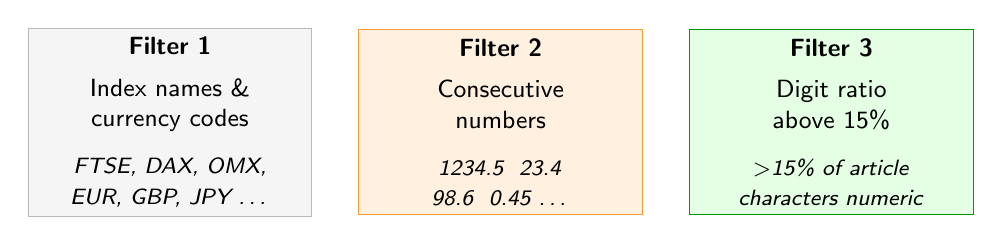
\begin{tikzpicture}[
    box1/.style={rectangle, draw=gray!55, fill=gray!8,
                minimum width=3.6cm, minimum height=2.2cm,
                font=\small\sffamily, align=center},
    box2/.style={rectangle, draw=orange!80, fill=orange!12,
                minimum width=3.6cm, minimum height=2.2cm,
                font=\small\sffamily, align=center},
    box3/.style={rectangle, draw=green!60!black, fill=green!10,
                minimum width=3.6cm, minimum height=2.2cm,
                font=\small\sffamily, align=center},
]

\node[box1] (f1) at (-4.2, 0) {
    \textbf{Filter 1}\\[4pt]
    Index names \&\\currency codes\\[6pt]
    \footnotesize\textit{FTSE, DAX, OMX,}\\
    \footnotesize\textit{EUR, GBP, JPY \ldots}
};

\node[box2] (f2) at (0, 0) {
    \textbf{Filter 2}\\[4pt]
    Consecutive\\numbers\\[6pt]
    \footnotesize\textit{1234.5\ \ 23.4}\\
    \footnotesize\textit{98.6\ \ 0.45 \ldots}
};

\node[box3] (f3) at (4.2, 0) {
    \textbf{Filter 3}\\[4pt]
    Digit ratio\\above 15\%\\[6pt]
    \footnotesize\textit{$>$15\% of article}\\
    \footnotesize\textit{characters numeric}
};

\end{tikzpicture}
\caption{Three contamination filters applied to remove financial market
         data tables incorrectly included in ProQuest exports.}
\label{fig:contamination_filters}
\end{figure}

\subsubsection*{Stopword Construction}

Stopword removal was applied in three different ways. The first two ways used 
the standard \texttt{sklearn} English stopword list and the 
\texttt{WordCloud} library defaults, which both handle common and generic terms. These alone were not enough for our data
because both the Financial Times articles and the Truth Social posts contain 
large volumes of topic specific noise that standard lists do not cover, which were visible in the word clouds.\\

To fix this a custom \texttt{extra} set was manually constructed from visual inspection of the word cloud. For the Financial Times articles, this included journalistic language
(\textit{said, according, told, added ...}), FT language 
(\textit{ft, reuters, financial, times ...}) and day and date terms that appear 
frequently in FT but carry no analytical signal (\textit{years, decade, today, tomorrow, Monday, Tuesday ...}). The word clouds were generated again and then more noisy irrelevant words were removed upon visual inspection, such as random letters, countries or names related to the articles (\textit{s, m, China, Russia, Trump, Putin ...}). This process was then iterated as many times as it needed to produce a valuable clean word cloud.\\

For the Truth Social posts, an additional 
\texttt{trump\_noise} set was constructed to remove authorial voice terms 
that dominate every post regardless of topic, such as 
(\textit{tremendous, incredible, fantastic, truly ...}). Other categories such as 
self referring terms  like (\textit{trump, donald, president, djt, realdonaldtrump}) and X (Twitter) language (\textit{rt, http, www, com, @ ...}) were also filtered out of the word cloud . The process used to refine the Financial Times word clouds was applied to the Truth Social posts to remove any noisy words (\textit{100, per, cent, bn, tn, don ...}), producing the finalised word cloud.

\subsection{Word Clouds}

Three major topics were selected for the word cloud analysis --- 
\texttt{russia\_ukraine}, \texttt{hamas\_israel}, \texttt{china\_taiwan}. These were chosen to reflect 
the broadest possible coverage of the geopolitical themes both positive and negative present in the 
Polymarket \texttt{geopolitics} trade data rather than focusing on the highest volume markets. This ensures the word clouds capture the full range of language used across different conflict types and political 
relationships.\\

Each topic was split into positive and negative subsets using the top and 
bottom quartile of the FinBERT \texttt{net\_score} distribution rather than 
a fixed cutoff, so the split is always relative to the tone of that specific 
topic. For a heavily negative topic like \texttt{hamas\_israel} shown in 
Figure \ref{fig:hamas_israel_dist}, the positive word cloud will contain the 
least negative articles rather than truly positive ones, while for a more 
balanced topic like \texttt{china\_taiwan} shown in Figure 
\ref{fig:china_taiwan_dist} the split will reflect a cleaner separation. 
This makes the word clouds more directly comparable across topics despite 
their different overall sentiment distributions.

\begin{figure}[H]
    \centering
    \includegraphics[width=\textwidth]{figures/hamas_israel_02_sentiment_histogram.png}
    \caption{FinBERT sentiment score distribution for \texttt{hamas\_israel}.}
    \label{fig:hamas_israel_dist}
\end{figure}

\begin{figure}[H]
    \centering
    \includegraphics[width=\textwidth]{figures/china_taiwan_02_sentiment_histogram.png}
    \caption{FinBERT sentiment score distribution for \texttt{china\_taiwan}.}
    \label{fig:china_taiwan_dist}
\end{figure}

\subsubsection*{Russia-Ukraine}

\begin{figure}[H]
    \centering
    \includegraphics[width=0.32\textwidth]{figures/russia_ukraine_04_wordcloud_all.png}
    \includegraphics[width=0.32\textwidth]{figures/russia_ukraine_05_wordcloud_positive.png}
    \includegraphics[width=0.32\textwidth]{figures/russia_ukraine_06_wordcloud_negative.png}
    \caption{Word clouds for \texttt{russia\_ukraine}. \newline Left: all articles. Centre: top quartile (most positive). Right: bottom quartile (most negative).}
    \label{fig:russia_ukraine_wordclouds}
\end{figure}

The \texttt{russia\_ukraine} word clouds in Figure~\ref{fig:russia_ukraine_wordclouds} 
show the FT framing the conflict through both a military and economic lens. 
The positive subset is dominated by \textit{deal, investment, support}, 
suggesting coverage of Western financial and military backing for Ukraine. 
The negative subset shifts towards \textit{gas, oil, prices, missile}, 
capturing the commodity disruption and active conflict narrative.\\

\subsubsection*{China-Taiwan}

\begin{figure}[H]
    \centering
    \includegraphics[width=0.32\textwidth]{figures/china_taiwan_04_wordcloud_all.png}
    \includegraphics[width=0.32\textwidth]{figures/china_taiwan_05_wordcloud_positive.png}
    \includegraphics[width=0.32\textwidth]{figures/china_taiwan_06_wordcloud_negative.png}
    \caption{Word clouds for \texttt{china\_taiwan}. \newline Left: all articles. Centre: top quartile (most positive). Right: bottom quartile (most negative).}
    \label{fig:china_taiwan_wordclouds}
\end{figure}

The \texttt{china\_taiwan} word clouds in Figure~\ref{fig:china_taiwan_wordclouds} 
show the FT covering this topic through a trade and technology lens rather 
than a military one. The positive subset is dominated by 
\textit{chip, global, defence, trade}, suggesting coverage 
focused on the technology industry and semiconductor supply chain story. 
The negative subset shifts towards \textit{tariff, officials, territory}, 
capturing the geopolitical tension.\\

\subsubsection*{Hamas-Israel}

\begin{figure}[H]
    \centering
    \includegraphics[width=0.32\textwidth]{figures/hamas_israel_04_wordcloud_all.png}
    \includegraphics[width=0.32\textwidth]{figures/hamas_israel_05_wordcloud_positive.png}
    \includegraphics[width=0.32\textwidth]{figures/hamas_israel_06_wordcloud_negative.png}
    \caption{Word clouds for \texttt{hamas\_israel}. \newline Left: all articles. Centre: top quartile (most positive). Right: bottom quartile (most negative).}
    \label{fig:hamas_israel_wordclouds}
\end{figure}

The \texttt{hamas\_israel} word clouds in Figure~\ref{fig:hamas_israel_wordclouds} 
are the most negative of the three topics, with a mean net sentiment score 
of $-0.455$. The positive subset is dominated by \textit{deal, ceasefire, 
release, hostages}, suggesting coverage focused on the diplomatic and 
negotiation process. The negative subset shifts to \textit{killed, strike, 
force, aid}, capturing the active conflict and civilian casualty 
narrative.\\

Across all three topics the positive and negative word cloud splits produce 
a clear separation, giving us confidence that the FinBERT scores are 
meaningfully picking up on different types of coverage.\\

\subsubsection*{Truth Social}

The Truth Social word clouds are analysed differently to the ProQuest ones. 
Because every post in the archive is by Trump, the positive and negative 
split reflects his speech style rather than news coverage of external events.

\begin{figure}[H]
    \centering
    \includegraphics[width=0.32\textwidth]{figures/ts_04_wordcloud_all.png}
    \includegraphics[width=0.32\textwidth]{figures/ts_05_wordcloud_positive.png}
    \includegraphics[width=0.32\textwidth]{figures/ts_06_wordcloud_negative.png}
    \caption{Word clouds for Truth Social posts. \newline Left: all posts. Centre: top quartile (most positive). Right: bottom quartile (most negative).}
    \label{fig:ts_wordclouds}
\end{figure}

Looking at the overall word cloud in Figure \ref{fig:ts_wordclouds}, the 
archive is dominated by terms like \textit{Biden, crooked, 
Fake, Radical, hoax}, showing that 
Trump's posts across the whole period were heavily focused on attacking 
political opponents.
The positive cloud moves away from the attack language and is instead dominated by words like 
\textit{Support, Defend, Protect, Ammendement, Secure}, suggesting the most positive posts were focused on patriotic and national strength language rather than specific events. 
The negative cloud is dominated by words like \textit{crooked, Fake, Hoax, fraud, crime, Rigged}, 
suggesting the most negative posts were focused on attacking the legal cases brought against Trump rather than any geopolitical topic. \\

Where the Financial Times splits separated different types of event coverage, the Truth Social split separates two different sides of Trump's posting style: patriotic strength language for positive posts and legal attack language for the negative ones.

\subsection{LDA Topic Modelling}

LDA was run on each set of articles to find hidden topics by looking at 
which words tend to appear together across documents. The number of topics 
k was chosen by starting at k=4 and then running the model again at k=5, 
visually inspecting the output tables to check whether the topics were 
separating cleanly or merging into each other. If two topics looked too 
similar we moved down to k=4, if one of the topics still looked too broad we 
moved up to k=6, and this was repeated until the topics were distinct 
enough to be interpretable.\\


After doing this all three FT topics from the LDA output showed a consistent pattern where the coverage of each conflict split into distinct threads.For \texttt{hamas\_israel} shown in Table \ref{tab:lda_hamas_israel}, the 
hostage negotiations and ground offensive dominated, showing coverage was 
focused on the operational detail of the conflict rather than the politics, 
with the keyword \textit{hostages} mapping directly to the Polymarket market 
``Will Hamas release any more hostages by October 31?'' in Table 
\ref{tab:polymarket_hamas_israel}. For \texttt{china\_taiwan} shown in Table 
\ref{tab:lda_china_taiwan}, the military posture and semiconductor topics 
emerged as two clearly separate threads, showing the tech war narrative had 
become its own distinct press beat separate from the military story, with the 
keyword \textit{semiconductor} mapping directly to the Polymarket market 
``Will Trump say `Semiconductor' or `Chip' during events with South Korean 
president on August 25?'' in Table \ref{tab:polymarket_china_taiwan}. In each 
case the LDA topics mapped directly to real Polymarket markets being traded 
during the same period, as shown in the tables below each LDA topic 
distribution. This shows our broad ProQuest searches were returning articles relevant to the markets being traded on polymarket.

\subsubsection*{Russia-Ukraine}

\begin{table}[H]
\centering
\begin{tabular}{llp{6cm}r}
\hline
\textbf{Topic} & \textbf{Label} & \textbf{Key Words} & \textbf{Articles} \\
\hline
T1 & Military Escalation \& Drone Warfare & defence, drones, nuclear, missiles, attacks & 475 \\
T2 & Ceasefire \& Peace Negotiations & peace, deal, talks, ceasefire, troops & 894 \\
T3 & Energy Politics \& Sanctions & gas, sanctions, lng, election, energy & 427 \\
T4 & NATO/EU Allied Defence Spending & defence, spending, poland, commission, bloc & 633 \\
T5 & Economic \& Energy Markets & oil, energy, prices, trade, investment, tariffs & 932 \\
\hline
\end{tabular}
\caption{LDA topic distribution for \texttt{russia\_ukraine} (k=5).}
\label{tab:lda_russia_ukraine}
\end{table}

\begin{table}[H]
\centering
\begin{tabular}{p{1cm}p{4.8cm}p{9.5cm}}
\hline
\textbf{Topic} & \textbf{Matched Keyword} & \textbf{Matched Polymarket Question} \\
\hline
T1 & nuclear & Will Zelensky say ``nuclear'' during his UN address? \\
T2 & peace, talks & Will the Vatican host Russia-Ukraine peace talks before September? \\
T3 & gas, lng & Will Trump say ``LNG'' or ``Natural Gas'' during events with South Korean president on August 25? \\
T4 & defence, spending & Will NATO members agree to raise defence spending targets before July? \\ %fake
T5 & oil & Will India agree to stop buying Russian oil by September 30? \\
\hline
\end{tabular}
\caption{Example Polymarket markets matched to \texttt{russia\_ukraine} LDA topics by keyword.}
\label{tab:polymarket_russia_ukraine}
\end{table}

\subsubsection*{Hamas-Israel}

\begin{table}[H]
\centering
\begin{tabular}{llp{6cm}r}
\hline
\textbf{Topic} & \textbf{Label} & \textbf{Key Words} & \textbf{Articles} \\
\hline
T1 & International Political Response \& Protests & government, jewish, party, political, university, police & 375 \\
T2 & Hostage Crisis \& Ground Offensive & hostages, ceasefire, killed, deal, release, offensive & 419 \\
T3 & Regional Escalation \& Strikes & strikes, lebanese, beirut, nuclear, region, attacks & 360 \\
T4 & Humanitarian Aid \& Peace Diplomacy & aid, humanitarian, peace, foreign, leaders & 308 \\
\hline
\end{tabular}
\caption{LDA topic distribution for \texttt{hamas\_israel} (k=4).}
\label{tab:lda_hamas_israel}
\end{table}

\begin{table}[H]
\centering
\begin{tabular}{p{2cm}p{4.8cm}p{9.5cm}}
\hline
\textbf{Topic} & \textbf{Matched Keyword} & \textbf{Matched Polymarket Question} \\
\hline
T1 & political, government & Will the ICC issue an arrest warrant for Netanyahu before the end of 2024? \\ %fake
T2 & hostages, release & Will Hamas release any more hostages by October 31? \\
T3 & nuclear & Will Trump say ``Nuclear'' during his February 4 press conference with Netanyahu? \\
T4 & aid & Will US airdrop aid into Gaza? \\
\hline
\end{tabular}
\caption{Example Polymarket markets matched to \texttt{hamas\_israel} LDA topics by keyword.}
\label{tab:polymarket_hamas_israel}
\end{table}

\subsubsection*{China-Taiwan}

\begin{table}[H]
\centering
\begin{tabular}{llp{6cm}r}
\hline
\textbf{Topic} & \textbf{Label} & \textbf{Key Words} & \textbf{Articles} \\
\hline
T1 & Indo-Pacific Security \& Korean Peninsula & security, korean, sanctions, peace, foreign & 109 \\
T2 & Financial Markets \& Economic Impact & markets, investors, growth, stocks, rates & 211 \\
T3 & Domestic Politics \& Cultural Tensions & party, election, tiktok, national, city & 218 \\
T4 & Military Posture \& South China Sea & defence, forces, allies, philippines, ministry & 310 \\
T5 & Semiconductor \& Tech War & chips, semiconductor, tariffs, manufacturing, supply & 237 \\
\hline
\end{tabular}
\caption{LDA topic distribution for \texttt{china\_taiwan} (k=5).}
\label{tab:lda_china_taiwan}
\end{table} 

\begin{table}[H]
\centering
\begin{tabular}{p{2cm}p{4.8cm}p{9.5cm}}
\hline
\textbf{Topic} & \textbf{Matched Keyword} & \textbf{Matched Polymarket Question} \\
\hline
T1 & korean & Will Trump say ``Semiconductor'' or ``Chip'' during events with South Korean president on August 25? \\
T2 & markets, investors & Will Chinese stock markets fall more than US markets before December? \\ %fake
T3 & tiktok & Will Trump say ``TikTok'' during Xi events on October 29? \\
T4 & philippines & China x Philippines military clash by June 30? \\
T5 & semiconductor & Will Trump say ``Semiconductor'' or ``Chip'' during events with South Korean president on August 25? \\
\hline
\end{tabular}
\caption{Example Polymarket markets matched to \texttt{china\_taiwan} LDA topics by keyword.}
\label{tab:polymarket_china_taiwan}
\end{table}

\subsubsection*{Truth Social}

\begin{table}[H]
\centering
\begin{tabular}{llp{6cm}r}
\hline
\textbf{Topic} & \textbf{Label} & \textbf{Key Words} & \textbf{Posts} \\
\hline
T1 & Legal Persecution \& Witch Hunt Narrative & judge, case, trial, attorney, corrupt, witch, interference & 1,809 \\
T2 & Electoral Polling \& Republican Primary & poll, ron, win, republicans, polls, desantis & 2,661 \\
T3 & Fake News \& Media Attacks & fake, fake news, live, join, tonight, watch & 2,219 \\
T4 & Russia Hoax \& Biden DOJ Corruption & russia, fbi, hoax, doj, documents, jack, rigged & 2,640 \\
T5 & Law Enforcement \& Immigration Policy & law, illegal, enforcement, security, women, serve & 1,735 \\
T6 & Second Amendment \& Border Siege & secure, amendment, siege, defend, protect, energy, texas & 1,103 \\
T7 & Biden-Kamala Attacks \& China Trade & biden, kamala, crooked, harris, china, dollars, worst & 3,384 \\
\hline
\end{tabular}
\caption{LDA topic distribution for Truth Social posts (k=7).}
\label{tab:lda_ts}
\end{table}


Looking at Truth Social posts in Table \ref{tab:lda_ts}, T7 Biden-Kamala Attacks and China Trade is the largest topic with 3,384 posts, showing that sustained attacks on Biden and Harris was the most consistent type of content across the archive of posts. T2 Electoral Polling and Republican Primary and T4 Russia Hoax and Biden DOJ Corruption are close behind with around 2,600 posts each, suggesting the primary race and Trump's attacks on the Justice Department were almost as dominant as the direct Biden attacks. Only T4 and T7 pick up any geopolitical content, with Russia appearing through the hoax framing and China through a trade attack angle, suggesting Trump's posts were focused almost entirely on domestic political attacks rather than geopolitical events, as we all know this is consistent with Trump's methods of using social media as an attack platform rather than for policy discussion, or discussing real world events.


\newpage
% =========================================================
\section{Machine Learning}
% =========================================================

\label{sec:ml}

The machine learning task is a \textbf{cold-start trading problem}. The key question is whether observable market and context features contain useful information \emph{beyond the Polymarket price itself}, and whether that information still works for wallets the model has never seen before.

% --------------------------------------
% FIGURE: Three-way divergence as motivating intuition
% Edit: box text, arrow labels, colours (fignavy / figblue / figgrey)
% --------------------------------------
\begin{figure}[H]
\centering
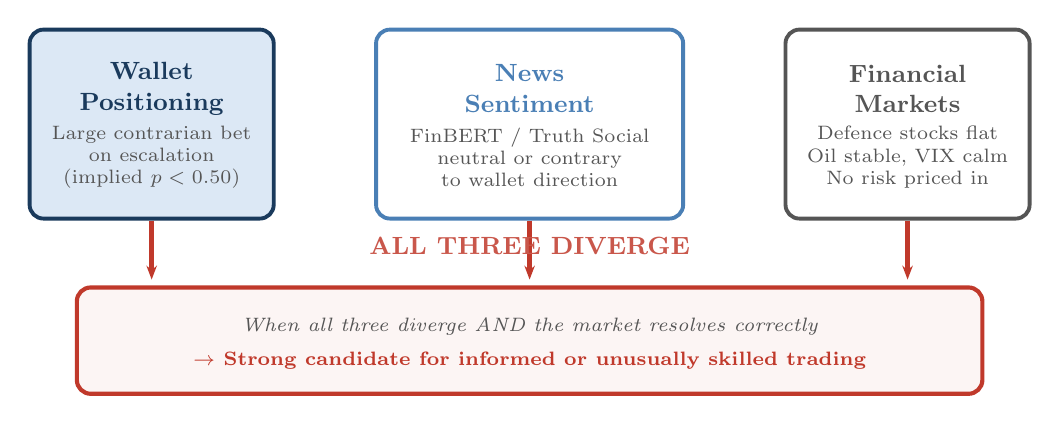
\begin{tikzpicture}[x=1cm,y=1cm]
%\node[anchor=south, text=fignavy, font=\Large\bfseries] at (5.6,4.95)
%  {Three-Way Divergence: The Core Signal};

\node[
  draw=fignavy,
  fill=figlblue,
  rounded corners=5pt,
  line width=1.4pt,
  minimum width=3.1cm,
  minimum height=2.4cm,
  align=center
] (wallet) at (0.8,2.2) {};
\node[text=fignavy, font=\small\bfseries, align=center] at ($(wallet.center)+(0,0.45)$)
  {Wallet\\Positioning};
\node[text=figgrey, font=\scriptsize, align=center] at ($(wallet.center)+(0,-0.42)$)
  {Large contrarian bet\\on escalation\\(implied $p<0.50$)};

\node[
  draw=figblue,
  fill=white,
  rounded corners=5pt,
  line width=1.4pt,
  minimum width=3.9cm,
  minimum height=2.4cm,
  align=center
] (news) at (5.6,2.2) {};
\node[text=figblue, font=\small\bfseries, align=center] at ($(news.center)+(0,0.45)$)
  {News\\Sentiment};
\node[text=figgrey, font=\scriptsize, align=center] at ($(news.center)+(0,-0.42)$)
  {FinBERT / Truth Social\\neutral or contrary\\to wallet direction};

\node[
  draw=figgrey,
  fill=white,
  rounded corners=5pt,
  line width=1.4pt,
  minimum width=3.1cm,
  minimum height=2.4cm,
  align=center
] (markets) at (10.4,2.2) {};
\node[text=figgrey, font=\small\bfseries, align=center] at ($(markets.center)+(0,0.45)$)
  {Financial\\Markets};
\node[text=figgrey, font=\scriptsize, align=center] at ($(markets.center)+(0,-0.42)$)
  {Defence stocks flat\\Oil stable, VIX calm\\No risk priced in};

\draw[-{Stealth[length=5pt]}, line width=1.6pt, color=figred] (wallet.south) -- ++(0,-0.75);
\draw[-{Stealth[length=5pt]}, line width=1.6pt, color=figred] (news.south) -- ++(0,-0.75);
\draw[-{Stealth[length=5pt]}, line width=1.6pt, color=figred] (markets.south) -- ++(0,-0.75);

\node[text=figred!85, font=\small\bfseries] at (5.6,0.65) {ALL THREE DIVERGE};

\node[
  draw=figred,
  fill=figred!5,
  rounded corners=5pt,
  line width=1.5pt,
  minimum width=11.5cm,
  minimum height=1.35cm,
  align=center
] (resultbox) at (5.6,-0.55) {};
\node[text=figgrey, font=\scriptsize\itshape, align=center] at ($(resultbox.center)+(0,0.18)$)
  {When all three diverge AND the market resolves correctly};
\node[text=figred, font=\scriptsize\bfseries, align=center] at ($(resultbox.center)+(0,-0.25)$)
  {$\rightarrow$ Strong candidate for informed or unusually skilled trading};
\end{tikzpicture}
\caption{Three-way divergence as a motivating intuition for feature design}
\label{fig:divergence}
\end{figure}
A candidate informed trade is one where the wallet's position, news sentiment, and cross-market signals point in different directions. This idea motivates part of the feature design, but it is not treated as the retained standalone model: the main empirical test below asks whether a combined market-and-context model adds value beyond price on previously unseen wallets.
\subsection{Objective, target and validation design}

%The primary target is \texttt{outcome\_correct}: did the buy-side position resolve in the wallet's favour? This binary label was chosen over the continuous \texttt{realized\_edge} as the training target for three reasons. First, every observation carries a clean 0/1 realisation, so the label is noise-free. Second, training on a continuous edge measure would compound two sources of noise -- the market price and the outcome -- magnifying heteroskedasticity and degrading gradient estimates. Third, a binary label is well suited to probabilistic calibration, which is the property we actually need: a well-calibrated $P(\text{correct} \mid \text{features})$ is directly interpretable as an implied-probability adjustment over the market price. ROC-AUC and PR-AUC are used as primary evaluation metrics in place of accuracy, because the outcome distribution is slightly skewed and we care about ranking quality across the full probability range rather than a single decision threshold.

The binary label \texttt{outcome\_correct} was selected over continuous \texttt{realised\_edge} as the training target because it provides a clean per-observation realisation with no noise compounding, and a calibrated $P(\text{correct} \mid \mathbf{x})$ is directly interpretable as a probability adjustment over the market price. All classifiers are fit with log-loss; ROC-AUC and PR-AUC are then used for evaluation because ranking quality matters more than a single hard threshold.

\begin{table}[H]
\centering
\small
\begin{tabularx}{\linewidth}{>{\bfseries}p{0.22\linewidth}L}
\toprule
Pipeline object & Definition and role \\
\midrule
Training target & \texttt{outcome\_correct}: binary resolution outcome for the buy-side wallet position. \\
Fitted loss & Log-loss for logistic regression and XGBoost. \\
Model-selection score & $0.5(\overline{\text{ROC-AUC}} + \overline{\text{PR-AUC}}) - \overline{\text{Brier}}$ on wallet-grouped CV folds inside the training sample only. \\
Economic ranking score & \texttt{predicted\_alpha = model\_prob - avg\_price}; realised value is checked with \texttt{realised\_edge = outcome\_correct - avg\_price}. \\
\bottomrule
\end{tabularx}
\caption{Target, fitted loss, model-selection score, and economic ranking metric used in the ML pipeline.}
\label{tab:score_stack}
\end{table}

Two derived measures are then used to judge economic usefulness:
\begin{itemize}[label=--]
    \item \texttt{realised\_edge = outcome\_correct - avg\_price}: how much better or worse the trade performed relative to the market-implied probability.
    \item \texttt{predicted\_alpha = model\_prob - avg\_price}: how much the model believes the trade is underpriced relative to the market.
\end{itemize}

The modelling table contains 394,279 wallet-position observations across 25,684 wallets and 1,794 markets. The main evaluation is a future, wallet-disjoint holdout, so the model cannot succeed by memorising specific traders.

\begin{table}[H]
\centering
\small
\begin{tabular}{lrrrr}
\toprule
Split & Rows & Wallets & Markets & Mean realised edge \\
\midrule
Train & 228,926 & 19,038 & 1,159 & 0.0039 \\
Cold test (unseen wallets) & 22,752 & 1,648 & 616 & 0.0023 \\
Warm test (seen later wallets) & 105,233 & 15,123 & 635 & -0.0012 \\
\bottomrule
\end{tabular}
\caption{Train/test structure for model building and validation}
\label{tab:test_train_struct}
\end{table}

% --------------------------------------
% FIGURE: Train/test timeline
% Edit: CUTOFF x-position (currently 7.08 = Sep 2025 on a 24-month axis)
%       bar colours, date labels, badge text
% --------------------------------------
\begin{figure}[H]
\centering
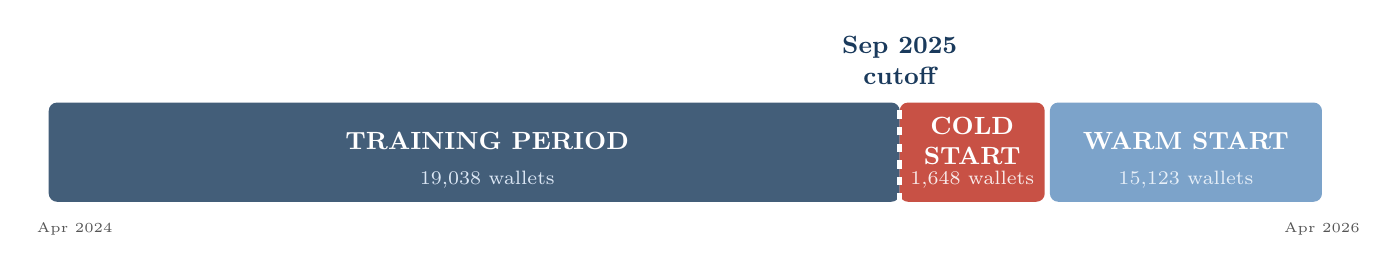
\begin{tikzpicture}[x=1.65cm,y=1.4cm]
\def\cutoff{6.55}
\pgfmathsetmacro{\coldw}{(12.75-\cutoff)*0.18}
\pgfmathsetmacro{\warmstart}{\cutoff+\coldw+0.04}

%\node[anchor=south, text=fignavy, font=\\bfseries, align=center] at (5.0,3.0)
%  {Train / Test Split Design and Wallet Disjointness};

\filldraw[fill=fignavy, draw=none, rounded corners=3pt, opacity=0.82] (0,0.6) rectangle (\cutoff,1.5);
\node[text=white, font=\small\bfseries] at ({(0.2+\cutoff)/2},1.15) {TRAINING PERIOD};
\node[text=figlblue, font=\scriptsize] at ({(0.2+\cutoff)/2},0.8) {19,038 wallets};

\filldraw[fill=figred, draw=none, rounded corners=3pt, opacity=0.88] (\cutoff,0.6) rectangle ({\cutoff+\coldw},1.5);
\node[text=white, font=\small\bfseries, align=center] at ({\cutoff+\coldw/2},1.15) {COLD\\START};
\node[text=figred!10, font=\scriptsize, align=center] at ({\cutoff+\coldw/2},0.8) {1,648 wallets};

\filldraw[fill=figblue, draw=none, rounded corners=3pt, opacity=0.72] (\warmstart,0.6) rectangle (9.8,1.5);
\node[text=white, font=\small\bfseries] at ({(\warmstart+9.8)/2},1.15) {WARM START};
\node[text=figlblue!70!white, font=\scriptsize] at ({(\warmstart+9.8)/2},0.8) {15,123 wallets};

\draw[white, dashed, line width=2.0pt] (\cutoff,0.6) -- (\cutoff,1.5);
\node[text=fignavy, font=\small\bfseries, align=center] at (\cutoff,1.88) {Sep 2025\\cutoff};

%\draw[draw=figgreen, fill=figgreen!8, rounded corners=4pt, line width=1.4pt] (1.0,2.42) rectangle (9,3.02);
%\node[text=figgreen, font=\small\bfseries, align=center] at (5.0,2.69)
%  {VERIFIED: Zero wallet overlap between training and cold-start test};

\node[text=figgrey, font=\tiny] at (0.2,0.35) {Apr 2024};
\node[text=figgrey, font=\tiny] at (9.8,0.35) {Apr 2026};
\end{tikzpicture}

\vspace{-1em}
\caption{Visualisation of train/test split design detailed in Table~\ref{tab:test_train_struct} above}
\label{fig:timeline}
\end{figure}

This design is materially stronger than a random split. It asks whether the model can generalise to new wallets in a later period, which is the relevant practical question.

\subsection{Model setup}

Three benchmark families were evaluated:
\begin{itemize}[label=--]
    \item \textbf{Market price only}: the baseline probability is simply the price paid.
    \item \textbf{Linear baseline}: logistic regression using market and context features.
    \item \textbf{Non-linear baseline}: XGBoost, estimated both with default-style settings \& Optuna tuning.
\end{itemize}

XGBoost was selected as the primary non-linear model for these reasons:
\begin{enumerate}
\item The feature set is a mix of continuous financial and sentiment signals combined with discrete market-level indicators. Gradient-boosted trees have well-documented empirical advantages over deep networks on precisely this type of data (Chen and Guestrin, 2016). 
\item Unlike logit, XGBoost captures non-linear dynamics and complex interactions between features. 
\item Unlike a neural network, it requires no normalisation, trains stably on the available data volume, and integrates naturally with Optuna via a compact hyperparameter space. 
\end{enumerate}
Logistic regression is retained as an interpretable baseline to verify that the XGBoost gains are genuinely non-linear rather than a product of additional features.\\

Model development was done on the training sample only using \edit{\texttt{GroupKFold} ($k{=}4$)} by wallet. This provides the validation methodology for hyperparameter selection: each fold's validation set contains wallets entirely absent from that fold's training split, which mirrors the cold-start structure of the main test. The cold unseen-wallet split is untouched until the final evaluation, while the warm split is retained as a secondary seen-wallet check. The retained primary model is the \textbf{tuned XGBoost using market and context features}.

\subsubsection*{Hyperparameter tuning}

\edit{Optuna with the TPE sampler was used to search over nine hyperparameters for 100 trials.} The objective was a composite of grouped CV scores: $0.5(\overline{\text{ROC-AUC}} + \overline{\text{PR-AUC}}) - \overline{\text{Brier}}$, balancing ranking quality against calibration error.

\begin{table}[H]
\centering
\scriptsize
\begin{tabular}{lrrrrrrrrr}
\toprule
 & \texttt{estimators} & \texttt{max\_depth} & \texttt{learn\_rate} & \texttt{child\_weight} & \texttt{subsample} & \texttt{colsample\_bytree} & L1 & L2 & \texttt{gamma} \\
\midrule
Baseline    & 250 & 4 & 0.050 & -- & 0.90 & 0.90 & -- & -- & -- \\
\edit{Optuna} & \edit{360} & \edit{6} & \edit{0.116} & \edit{3} & \edit{0.697} & \edit{0.970} & \edit{0.00023} & \edit{0.00042} & \edit{1.180} \\
\bottomrule
\end{tabular}
\caption{\edit{Base and Optuna-selected hyperparameters for XGBoost (base uses default XGB regularisation)}}
\label{tab:hyperparams}
\end{table}

Figure~\ref{fig:optuna_trials} shows the grouped cross-validation objective improves quickly across the search and then stabilises, indicating convergence toward a consistent high-performing region of the hyperparameter space. The best trials cluster around deeper trees with stronger regularisation, which suggests that the signal is interaction-rich but still requires discipline to generalise beyond the training wallets.

\begin{figure}[H]
\centering
\includegraphics[width=\textwidth,height=0.6\textheight,keepaspectratio]{figures/optuna_tuning_trials.png}
\caption{Trial-level Optuna diagnostics for the retained XGBoost model. Darker points indicate stronger grouped-CV performance and the red star marks the selected best trial.}
\label{fig:optuna_trials}
\end{figure}


The selected parameters reflect that balance. A higher max\_depth allows the model to capture more complex interactions, while gamma = 1.39 and min\_child\_weight = 6 constrain unnecessary or low-support splits. This means the tuned model is more expressive than the baseline, but not simply more flexible in an uncontrolled way. The higher learning rate is therefore consistent with a more tightly regularised tree structure rather than a looser specification.\\[-1em]
\begin{table}[H]
\centering
\small
\begin{tabular}{lrrrr}
\toprule
Model comparison (market \& context features) & ROC-AUC & PR-AUC & Brier & Log-loss \\
\midrule
%\multicolumn{6}{c}{\textcolor{blue}{Model comparison (market + context features)}} \\[2pt]
Baseline XGBoost            & 0.9703 & 0.9765 & 0.0688 & 0.2311 \\
Tuned XGBoost          & 0.9983 & 0.9986 & 0.0158 & 0.0659 \\
\bottomrule
\end{tabular}
\caption{\edit{Grouped cross-validation performance for the baseline and tuned XGBoost specifications}}
\label{tab:ml_cv_results}
\end{table}

\edit{Although the tuned model strongly outperforms the baseline in grouped CV on ROC-AUC (0.9983 vs 0.9703), it is weaker on the realised unseen-wallet test sample (0.9534 versus 0.9577, in Table~\ref{tab:ml_main_results}). The tuned model is still retained as the primary specification because it was selected ex ante using grouped CV and a predefined composite objective, whereas switching models after seeing the holdout result would introduce look-ahead bias. Both models remain comfortably above the market-price benchmark.}

%Figure~\ref{fig:optuna_trials} makes the search path more transparent than the best-parameter table alone. Performance improves sharply by the middle of the search, then stabilises around a family of deeper, more strongly regularised trees. The tuned configuration therefore appears to be selecting an interaction-rich but still disciplined specification, rather than simply chasing a high-complexity corner of the space. The larger \texttt{max\_depth} (6 vs 4) suggests the signal has moderately deep feature interactions, while the high \texttt{gamma} (1.39) simultaneously prunes shallow nodes, acting as a structural regulariser. The elevated \texttt{min\_child\_weight} (6) imposes a further variance penalty, preventing the model from splitting on small wallet subgroups that may not generalise. The learning rate increased (0.113 vs 0.050) because the added regularisation absorbs the variance that a slower rate would otherwise control.
%
%On the grouped CV folds, the tuned model substantially outperforms the baseline (CV ROC-AUC: 0.9968 vs 0.9703). On the held-out test set, however, the tuned model marginally underperforms the baseline on all four metrics (ROC-AUC: 0.9552 vs 0.9577; Table~\ref{tab:ml_main_results}). This reversal is expected: the CV composite objective was optimised jointly over ROC-AUC, PR-AUC and Brier score, whereas the test set is a single sample. The tuned model was retained as primary precisely because it was selected \emph{ex ante} from CV results, without any access to the test set; reverting to the baseline after observing the test outcome would introduce look-ahead bias into the model selection process. Both models improve substantially on the market baseline of 0.9432.

\subsection{Main results}

\vspace{-1em}
\begin{table}[H]
\centering
\small
\begin{tabular}{lcrrrr}
\toprule
Model comparison (market \& context features) & Features & ROC-AUC & PR-AUC & Brier & Log-loss \\
\midrule
%\multicolumn{6}{c}{\textcolor{blue}{Model comparison (market + context features)}} \\[2pt]
Market price only            & 1  & 0.9432 & 0.9496 & 0.0985 & 0.3230 \\
Logistic regression          & 28 & 0.9442 & 0.9517 & 0.0948 & 0.3119 \\
Baseline XGBoost             & 28 & 0.9577 & 0.9627 & 0.0818 & 0.2653 \\
Tuned XGBoost (primary)      & 28 & 0.9534 & 0.9583 & 0.0875 & 0.2950 \\
Tuned XGBoost (full feature set) & 31 & 0.9533 & 0.9586 & 0.0876 & 0.2950 \\
Tuned XGBoost (divergence only) & 24 & 0.8051 & 0.7958 & 0.1860 & 0.6179 \\
\bottomrule	

%\multicolumn{6}{c}{\textcolor{blue}{Feature-family ablation (tuned XGBoost)}} \\[2pt]
Feature-family ablation (tuned XGBoost) & Features & ROC-AUC & PR-AUC & Brier & Log-loss \\
\midrule
Market price only            &  1 & 0.9432 & 0.9496 & 0.0985 & 0.3230 \\
History only                 &  5 & \edit{0.9416} & \edit{0.9486} & \edit{0.0980} & \edit{0.3159} \\
Context only                 & 27 & \edit{0.9526} & \edit{0.9574} & \edit{0.0889} & \edit{0.3001} \\
Full cold-start set          & 31 & \edit{0.9533} & \edit{0.9586} & \edit{0.0876} & \edit{0.2950} \\
\bottomrule
\end{tabular}
\caption{Cold-start performance, retained-model comparison, and feature set ablation on unseen wallets}
\label{tab:ml_main_results}
\end{table}

Every machine learning model that retains price information improves on the market baseline, supporting the hypothesis that incremental signal exists beyond price. The tuned model is retained because it was selected \emph{ex ante} via grouped CV rather than after observing the test outcome.\\[-1em]

We also observe that the \textbf{context-only} model beats both the market benchmark and the history-only specification, showing the result is not simply ``good wallets stay good''. The divergence-only benchmark is materially weaker than the retained market-and-context model, so divergence is best interpreted as one useful contextual ingredient rather than the primary standalone signal.

%\begin{table}[H]
%\centering
%\small
%\begin{tabular}{lrrrrr}
%\toprule
%Feature set & Features & ROC-AUC & PR-AUC & Brier & Log-loss \\
%\midrule
%Market price only & 1 & 0.9432 & 0.9496 & 0.0985 & 0.3230 \\
%History only & 5 & 0.9428 & 0.9496 & 0.0970 & 0.3134 \\
%Context only & 27 & 0.9512 & 0.9564 & 0.0907 & 0.3017 \\
%Full cold-start set & 31 & 0.9550 & 0.9597 & 0.0850 & 0.2823 \\
%\bottomrule
%\end{tabular}
%\caption{Feature-family ablation on the cold-start holdout.}
%\label{tab:ml_ablation}
%\end{table}

\subsection{Economic value and robustness}

\vspace{-1em}
\begin{table}[H]
\centering
\small
\begin{tabular}{lrrrr}
\toprule
Selection rule & Rows & Hit rate & Mean market probability & Mean realised edge \\
\midrule
All cold-start trades & \ColdAllRows & \ColdAllHit & \ColdAllProb & \ColdAllEdge \\
Top 10\% by divergence-only alpha & \DivTopRows & \DivTopHit & \DivTopProb & \DivTopEdge \\
Top 10\% by main model alpha & \MainTopRows & \MainTopHit & \MainTopProb & \MainTopEdge \\
Top 10\% highest market price & \PriceTopRows & \PriceTopHit & \PriceTopProb & \PriceTopEdge \\
\bottomrule
\end{tabular}
\caption{Economic ranking quality on the unseen-wallet test set.}
\label{tab:ml_alpha}
\end{table}

%Reporting both hit rate and mean market probability makes clear that raw accuracy alone is not the business objective.
% --------------------------------------
% FIGURE: Alpha monotonicity — bar chart + line chart
% Edit: coordinates (edge values, hit rates, market probs), colours
% Labels: {All,T50,T40,T30,T20,T10} with symbolic x coords
% --------------------------------------
\begin{figure}[H]
\centering
\begin{adjustbox}{max width=\textwidth}
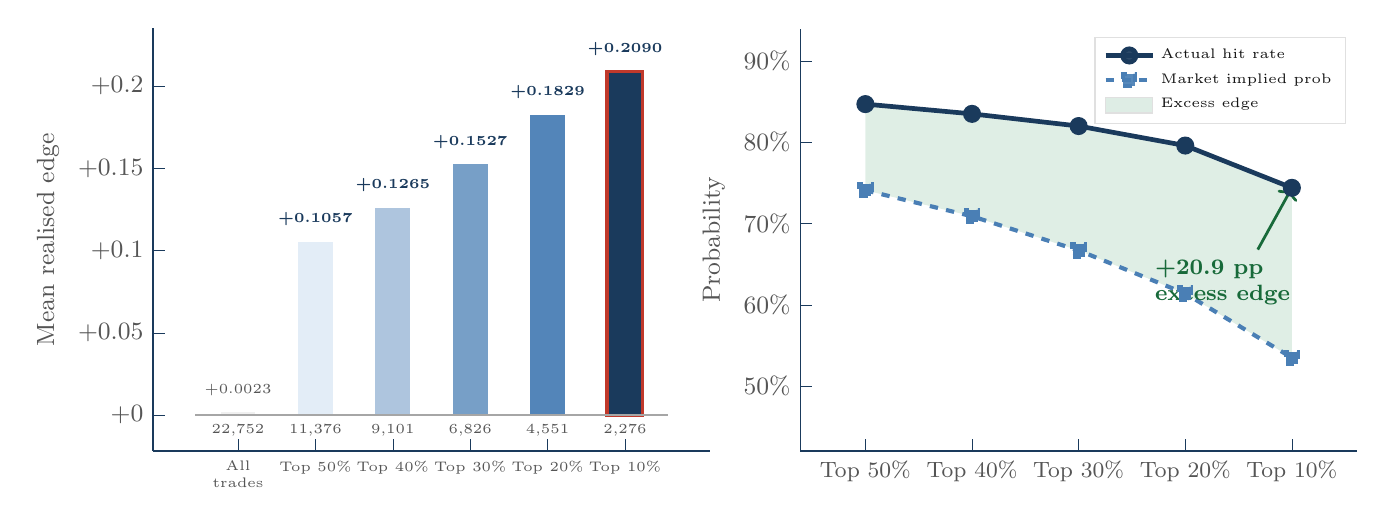
\begin{tikzpicture}
\begin{groupplot}[
  group style={group size=2 by 1, horizontal sep=1.15cm},
  fig style,
  width=8.65cm,
  height=6.95cm,
  enlarge x limits=0.08,
]

% =========================================================
% LEFT PANEL: Realized edge by selection
% =========================================================
\nextgroupplot[
  %title={Realized Edge by Selection},
  title style={font=\normalsize\bfseries, yshift=2pt},
  xmin=-0.6, xmax=5.6,
  ymin=-0.022, ymax=0.235,
  xtick={0,1,2,3,4,5},
  xticklabels={
    {{All\\trades}},
    {{Top 50\%}},
    {{Top 40\%}},
    {{Top 30\%}},
    {{Top 20\%}},
    {{Top 10\%}}
  },
  xticklabel style={font=\tiny, align=center},
  ylabel={Mean realised edge},
  ylabel style={align=center, font=\small},
  ytick={0,0.05,0.10,0.15,0.20},
  yticklabel={+\pgfmathprintnumber[fixed,precision=2]{\tick}},
  tick label style={font=\small},
]

\addplot[ybar, bar width=13pt, fill=figmgrey, draw=white] coordinates {(0,0.0023)};
\addplot[ybar, bar width=13pt, fill=figlblue!80!white, draw=white] coordinates {(1,0.1057)};
\addplot[ybar, bar width=13pt, fill=figblue!45!white, draw=white] coordinates {(2,0.1265)};
\addplot[ybar, bar width=13pt, fill=figblue!75!white, draw=white] coordinates {(3,0.1527)};
\addplot[ybar, bar width=13pt, fill=figblue!95!white, draw=white] coordinates {(4,0.1829)};
\addplot[ybar, bar width=13pt, fill=fignavy, draw=figred, line width=1.1pt] coordinates {(5,0.2090)};

\draw[black!35, line width=0.4pt] (axis cs:-0.55,0) -- (axis cs:5.55,0);

\node[text=figgrey, font=\tiny] at (axis cs:0,0.0023) [above=2pt] {+0.0023};
\node[text=fignavy, font=\tiny\bfseries] at (axis cs:1,0.1057) [above=2pt] {\edit{+0.1057}};
\node[text=fignavy, font=\tiny\bfseries] at (axis cs:2,0.1265) [above=2pt] {\edit{+0.1265}};
\node[text=fignavy, font=\tiny\bfseries] at (axis cs:3,0.1527) [above=2pt] {\edit{+0.1527}};
\node[text=fignavy, font=\tiny\bfseries] at (axis cs:4,0.1829) [above=2pt] {\edit{+0.1829}};
\node[text=fignavy, font=\tiny\bfseries] at (axis cs:5,0.2090) [above=2pt] {\edit{+0.2090}};

\node[text=figgrey, font=\tiny] at (axis cs:0,-0.0095) {22,752};
\node[text=figgrey, font=\tiny] at (axis cs:1,-0.0095) {11,376};
\node[text=figgrey, font=\tiny] at (axis cs:2,-0.0095) {9,101};
\node[text=figgrey, font=\tiny] at (axis cs:3,-0.0095) {6,826};
\node[text=figgrey, font=\tiny] at (axis cs:4,-0.0095) {4,551};
\node[text=figgrey, font=\tiny] at (axis cs:5,-0.0095) {2,276};

% =========================================================
% RIGHT PANEL: Hit rate vs market implied probability
% =========================================================
\nextgroupplot[
  %title={Hit Rate vs. Market Implied Probability},
  title style={font=\normalsize\bfseries, yshift=2pt},
  xmin=0.75, xmax=5.25,
  ymin=42, ymax=94,
  xtick={1,2,3,4,5},
  xticklabels={
    {{Top 50\%}},
    {{Top 40\%}},
    {{Top 30\%}},
    {{Top 20\%}},
    {{Top 10\%}}
  },
  xticklabel style={font=\footnotesize},
  ylabel={Probability},
  ylabel style={font=\small},
  ytick={50,60,70,80,90},
  yticklabel={\pgfmathprintnumber[fixed,precision=0]{\tick}\%},
  tick label style={font=\small},
  legend style={
    font=\tiny,
    draw=black!12,
    fill=white,
    fill opacity=0.92,
    at={(0.98,0.98)},
    anchor=north east
  },
  legend cell align=left,
]

\addplot[
  name path=hitrate,
  fignavy,
  line width=1.7pt,
  mark=*,
  mark size=2.4pt
] coordinates {
  (1,84.7) (2,83.5) (3,82.0) (4,79.6) (5,74.4)
};
\addlegendentry{Actual hit rate}

\addplot[
  name path=marketprob,
  figblue,
  dashed,
  line width=1.5pt,
  mark=square*,
  mark size=2.2pt
] coordinates {
  (1,74.1) (2,70.9) (3,66.7) (4,61.4) (5,53.5)
};
\addlegendentry{Market implied prob}

\addplot[
  draw=none,
  fill=figgreen,
  fill opacity=0.14
] fill between[of=hitrate and marketprob];
\addlegendentry{Excess edge}

\draw[->, line width=1.0pt, color=figgreen!80!black]
  (axis cs:4.68,66.8) -- (axis cs:5.0,74.4);

\node[
  text=figgreen!80!black,
  font=\footnotesize\bfseries,
  align=left
] at (axis cs:4.35,62.8)
{\edit{+20.9 pp}\\\edit{excess edge}};

\end{groupplot}

% =========================================================
% Shared title
% =========================================================
%\node[
%  anchor=south,
%  text=fignavy,
%  font=\large\bfseries,
%  align=center
%] at ($(group c1r1.north west)!0.5!(group c2r1.north east)+(0,0.72cm)$)
%{Economic Value: Realized Edge Increases Monotonically with Model Confidence};

\end{tikzpicture}
\end{adjustbox}
\caption{\edit{Left: mean realised edge rises monotonically as the model's selection threshold tightens. Right: in the top-10\% slice the model selects trades at an average implied probability of 53.5\%, yet those trades resolve correctly 74.4\% of the time, a 20.9 percentage-point excess over the market price.}}
\label{fig:alpha}
\end{figure}



\begin{figure}[H]
    \centering
    \includegraphics[width=0.86\linewidth]{figures/cold_start_evaluation.png}
    \caption{Cold-start model evaluation on unseen wallets.}
    \label{fig:cold_start_eval}
\end{figure}

The model improves on the market benchmark in ranking, calibration and realised-edge concentration. The result is also reasonably robust:
\begin{itemize}[label=--]
    \item \edit{Across three alternative unseen-wallet holdouts (seeds 11, 42, 99), average ROC-AUC rises from 0.9422 for the market benchmark to 0.9525 for the model.}
    \item \edit{Wallet-level bootstrap inference gives strictly positive 95\% confidence intervals for all four metrics, with one-sided bootstrap $p = 0.0003$ in each case.}
    \item \edit{A stricter entry-date walk-forward audit still shows weighted uplift: ROC $+0.0106$, PR $+0.0082$, Brier improvement $+0.0092$, and log-loss improvement $+0.0278$.}
\end{itemize}

\subsubsection*{What drives the prediction}

To move beyond rank-ordered gain importance, we compute exact TreeSHAP
values on the cold-start test set for the retained context model. Each
point in Figure~\ref{fig:shap-beeswarm} is one unseen-wallet trade;
horizontal position is the feature's contribution to the log-odds of
\texttt{outcome\_correct}, and colour encodes the feature value from
low (blue) to high (red).

\begin{figure}[ht]
    \centering
    \includegraphics[width=0.65\linewidth]{figures/shap_beeswarm.png}
    \caption{SHAP beeswarm on the cold-start test set. Features are
    ordered top-to-bottom by mean $|\text{SHAP}|$. Red points indicate
    high feature values, blue points low feature values.}
    \label{fig:shap-beeswarm}
\end{figure}

Three observations follow. First, avg\_price is the dominant
driver by mean $|\text{SHAP}|$ and the red--blue ordering is strictly
monotonic: higher market-implied probability pushes the predicted
\(P(\text{correct})\) upward, and lower price pushes it downward. This
is the calibrated behaviour a useful model should show against a
near-efficient price benchmark, and it confirms that the remaining
features are not being used to systematically fight the market.

Second, the sentiment and divergence family
(ts\_weekly\_score, ts\_weekly\_divergence,
 divergence\_score, ft\_sentiment\_score\_z) sits in
the next tier of mean $|\text{SHAP}|$. Aligned sentiment shifts the
prediction in the direction of the wallet's position, while divergence
between wallet direction and prevailing sentiment shifts it against.
These features therefore add directional signal beyond price, which is
consistent with the context-only ablation in Table~\ref{tab:ml_main_results}
outperforming the history-only specification on unseen wallets.

Third, the trade-context features (log\_net\_usd,
hours\_before, log\_market\_volume) exhibit
non-monotonic SHAP distributions, with both tails of the feature
distribution producing contributions of either sign. This is precisely
the interaction structure a linear model cannot represent, and it
empirically supports the choice of XGBoost over the logistic-regression
baseline rather than that choice being purely \emph{ex ante}. Taken
together, the beeswarm shows that the cold-start uplift is attributable
to a small number of interpretable feature families acting in
finance-consistent directions, not to any single opaque signal.


% --------------------------------------
% FIGURE: Bootstrap CI forest plot (horizontal bars + error bars)
% Edit: observed uplifts, ci_lo, ci_hi; x-axis limits
% --------------------------------------
\vspace{1.5em}
\begin{figure}[H]
\centering
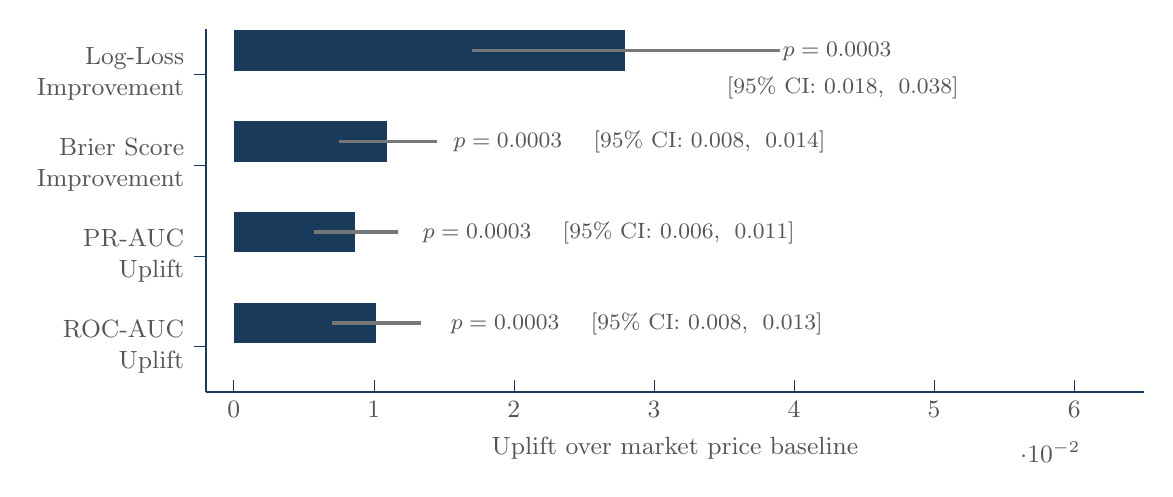
\begin{tikzpicture}
\begin{axis}[
  fig style,
  width=13.5cm,
  height=6.2cm,
  xbar,
  xmin=-0.002, xmax=0.065,
  ymin=-0.5, ymax=3.5,
  y dir=reverse,
  ytick={0,1,2,3},
  yticklabels={
    {{Log-Loss\\Improvement}},
    {{Brier Score\\Improvement}},
    {{PR-AUC\\Uplift}},
    {{ROC-AUC\\Uplift}}
  },
  yticklabel style={font=\small, align=right},
  xtick={0,0.01,0.02,0.03,0.04,0.05,0.06},
  xticklabel={\pgfmathprintnumber[fixed,precision=2]{\tick}},
  tick label style={font=\small},
  xlabel={Uplift over market price baseline},
  xlabel style={font=\small},
%  title={Bootstrap Inference: Model Uplift over Market Baseline\\(wallet-clustered resampling, 3{,}000 iterations, one-tailed $p$-values)},
  title style={text=fignavy, font=\normalsize\bfseries, align=center},
]
\addplot[black!40, dashed, line width=0.9pt] coordinates {(0,-0.5) (0,3.5)};
\addplot[
  xbar,
  bar width=15pt,
  fill=fignavy,
  draw=white,
  error bars/.cd,
    x dir=both,
    x explicit,
    error bar style={figgrey!80, line width=1.3pt},
    error mark options={figgrey!80, line width=1.3pt, mark size=3.5pt, mark=|},
] coordinates {
  (0.0280,0) +- (0.0103,0.0095)
  (0.0110,1) +- (0.0028,0.0027)
  (0.0087,2) +- (0.0023,0.0025)
  (0.0102,3) +- (0.0025,0.0027)
};

\node[text=figgrey, font=\footnotesize, anchor=west] at (axis cs:0.0385,-0.25) {\edit{$p = 0.0003$}};
\node[text=figgrey, font=\footnotesize, anchor=west] at (axis cs:0.0345,0.15) {\edit{[95\% CI: 0.018,\; 0.038]}};
\node[text=figgrey, font=\footnotesize, anchor=west] at (axis cs:0.0150,0.75) {\edit{$p = 0.0003$ \quad [95\% CI: 0.008,\; 0.014]}};
\node[text=figgrey, font=\footnotesize, anchor=west] at (axis cs:0.0128,1.75) {\edit{$p = 0.0003$ \quad [95\% CI: 0.006,\; 0.011]}};
\node[text=figgrey, font=\footnotesize, anchor=west] at (axis cs:0.0148,2.75) {\edit{$p = 0.0003$ \quad [95\% CI: 0.008,\; 0.013]}};
\end{axis}

%\node[anchor=north, text=figgrey, font=\small\itshape, align=center]
%  at ($(current bounding box.south)+(0,-0.45cm)$)
%  {Intervals based on resampling wallets, not individual rows -- the correct inference unit for clustered trade data.};
\end{tikzpicture}
\caption{Bootstrap confidence intervals for metric uplift over the market baseline
(3,000 iterations).}
\label{fig:bootstrap}
\end{figure}

Intervals are based on resampled wallets, not rows, a better inference unit for clustered trade data.
We can see all four uplifts are statistically significant and all lower confidence bounds are strictly above zero.

\vspace{1.25em}
\begin{mdframed}[linewidth=0.6pt, backgroundcolor=ucdblue]
\vspace{0.5em}
\textcolor{white}{\textbf{In conclusion,} observable market and context features contain
incremental predictive signal beyond price, and that signal remains useful on the
unseen wallets}
\vspace{0.5em}
\end{mdframed}

\newpage

% =========================================================
\section{Business Analysis}
% =========================================================
\label{sec:business}

\subsection{What the model is useful for}

The model is most useful as a \textbf{ranking tool}, not as a blanket rule to trade everything. On the full cold-start test set the average realised edge is close to zero, so the commercial value comes from \textbf{screening} and \textbf{capital allocation} rather than from raw prediction alone.

As prediction markets are already fairly efficient, a profitable process should not try to overturn every price. Instead, we try to identify a set of trades where the market appears slightly mispriced and concentrate risk there.

% --------------------------------------
% FIGURE: Trade screening funnel
% Edit: stage labels, n values, edge values, band heights/widths
% The funnel is drawn as trapezoids using \fill with path coordinates.
% Each stage: (y, half-width-top, half-width-bottom, label-left, label-right, fill)
% --------------------------------------
\begin{figure}[H]
\centering
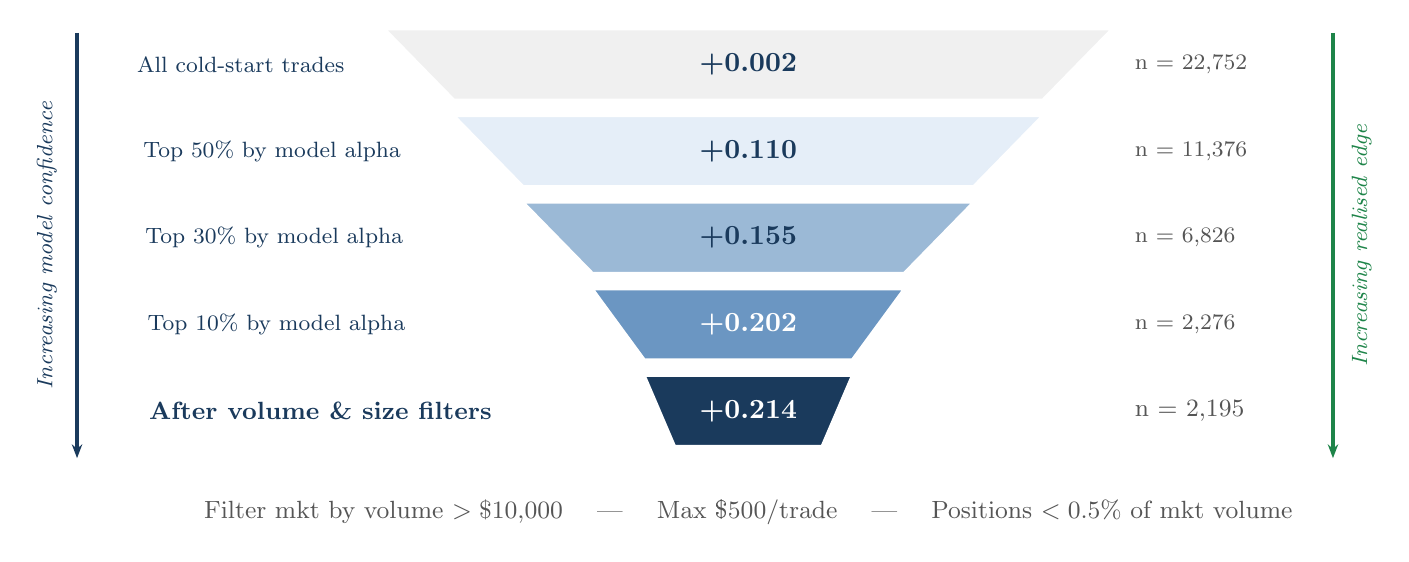
\begin{tikzpicture}[x=1.1cm,y=1cm]
%\node[anchor=south, text=fignavy, font=\small\bfseries, align=center] at (5,6.15)
%  {Trade Screening Funnel: From Raw Trades to High-Conviction Selection};

\fill[figmgrey, draw=white, line width=1.0pt] (0.8,5.75) -- (9.2,5.75) -- (8.4,4.85) -- (1.6,4.85) -- cycle;
\node[text=fignavy, font=\footnotesize] at (0.45,5.30) [anchor=east] {All cold-start trades};
\node[text=figgrey, font=\footnotesize, align=left] at (9.35,5.30) [anchor=west] {n = 22,752};
\node[text=fignavy, font=\normalsize\bfseries] at (5,5.30) {+0.002};

\fill[figlblue!75!white, draw=white, line width=1.0pt] (1.6,4.65) -- (8.4,4.65) -- (7.6,3.75) -- (2.4,3.75) -- cycle;
\node[text=fignavy, font=\footnotesize] at (1.1,4.20) [anchor=east] {Top 50\% by model alpha};
\node[text=figgrey, font=\footnotesize, align=left] at (9.35,4.20) [anchor=west] {n = 11,376};
\node[text=fignavy, font=\normalsize\bfseries] at (5,4.20) {+0.110};

\fill[figblue!55!white, draw=white, line width=1.0pt] (2.4,3.55) -- (7.6,3.55) -- (6.8,2.65) -- (3.2,2.65) -- cycle;
\node[text=fignavy, font=\footnotesize] at (1.125,3.10) [anchor=east] {Top 30\% by model alpha};
\node[text=figgrey, font=\footnotesize, align=left] at (9.35,3.10) [anchor=west] {n = 6,826};
\node[text=fignavy, font=\normalsize\bfseries] at (5,3.10) {+0.155};

\fill[figblue!82!white, draw=white, line width=1.0pt] (3.2,2.45) -- (6.8,2.45) -- (6.2,1.55) -- (3.8,1.55) -- cycle;
\node[text=fignavy, font=\footnotesize] at (1.15,2.00) [anchor=east] {Top 10\% by model alpha};
\node[text=figgrey, font=\footnotesize, align=left] at (9.35,2.00) [anchor=west] {n = 2,276};
\node[text=white, font=\normalsize\bfseries] at (5,2.00) {+0.202};

\fill[fignavy, draw=white, line width=1.0pt] (3.8,1.35) -- (6.2,1.35) -- (5.85,0.45) -- (4.15,0.45) -- cycle;
\node[text=fignavy, font=\small\bfseries] at (2.15,0.90) [anchor=east] {After volume \& size filters};
\node[text=figgrey, font=\small, align=left] at (9.35,0.90) [anchor=west] {\edit{n = 2,195}};
\node[text=white, font=\normalsize\bfseries] at (5,0.90) {\edit{+0.214}};

\draw[-{Stealth[length=5pt]}, line width=1.5pt, color=fignavy] (-2.75,5.7) -- (-2.75,0.30);
\node[text=fignavy, font=\footnotesize\itshape, rotate=90, align=center] at (-3.1,3.0)
  {Increasing model confidence};

\draw[-{Stealth[length=5pt]}, line width=1.5pt, color=figgreen] (11.75,5.7) -- (11.75,0.30);
\node[text=figgreen, font=\footnotesize\itshape, rotate=90, align=center] at (12.08,3.0)
  {Increasing realised edge};

\node[anchor=north, text=figgrey, font=\small, align=center] at (5,-0.10)
  {Filter mkt by volume $> \$10{,}000$ \quad | \quad Max \$500/trade \quad | \quad Positions $< 0.5\%$ of mkt volume};
\end{tikzpicture}
\caption{Trade screening funnel.}
\label{fig:funnel}
\end{figure}

\edit{The model narrows 22,752 cold-start trades to 2,195 high-conviction positions after volume, sizing, and participation filters. Realised edge rises at every stage, confirming that model alpha is a meaningful screening criterion rather than a restatement of the market price.}
\subsection{Commercial interpretation of the results}

In our view, the business value of the model comes from the following:

\begin{enumerate}
    \item \textbf{The edge is concentrated.} The top 10\% of trades by main-model alpha have a realised edge of $+\MainTopEdge$, while the full cold-start set is essentially flat at $\ColdAllEdge$.
    \item \textbf{High hit rate alone is not enough.} The top 10\% highest-price contracts resolve correctly 99.52\% of the time, but market already prices them at 98.38\%, leaving only $\PriceTopEdge$ realised edge.
    \item \textbf{Divergence alone is not the business signal.} The divergence-only top decile is nearly flat at $\DivTopEdge$, so the commercial value comes from combining price with broader context rather than from a standalone divergence heuristic.
\end{enumerate}

For a trading or research team, this means the model can be used to prioritise which contracts deserve analyst attention, rank candidate trades before capital is allocated, flag cases where public sentiment and cross-market context disagree with price, and improve discipline by comparing discretionary trades to a data-driven alpha score rather than to raw hit rate alone.

% --------------------------------------
% FIGURE: Screening diagnostics
% LEFT: hit rate versus market-implied probability
% RIGHT: realised edge in percentage points
% --------------------------------------
\begin{figure}[H]
\centering
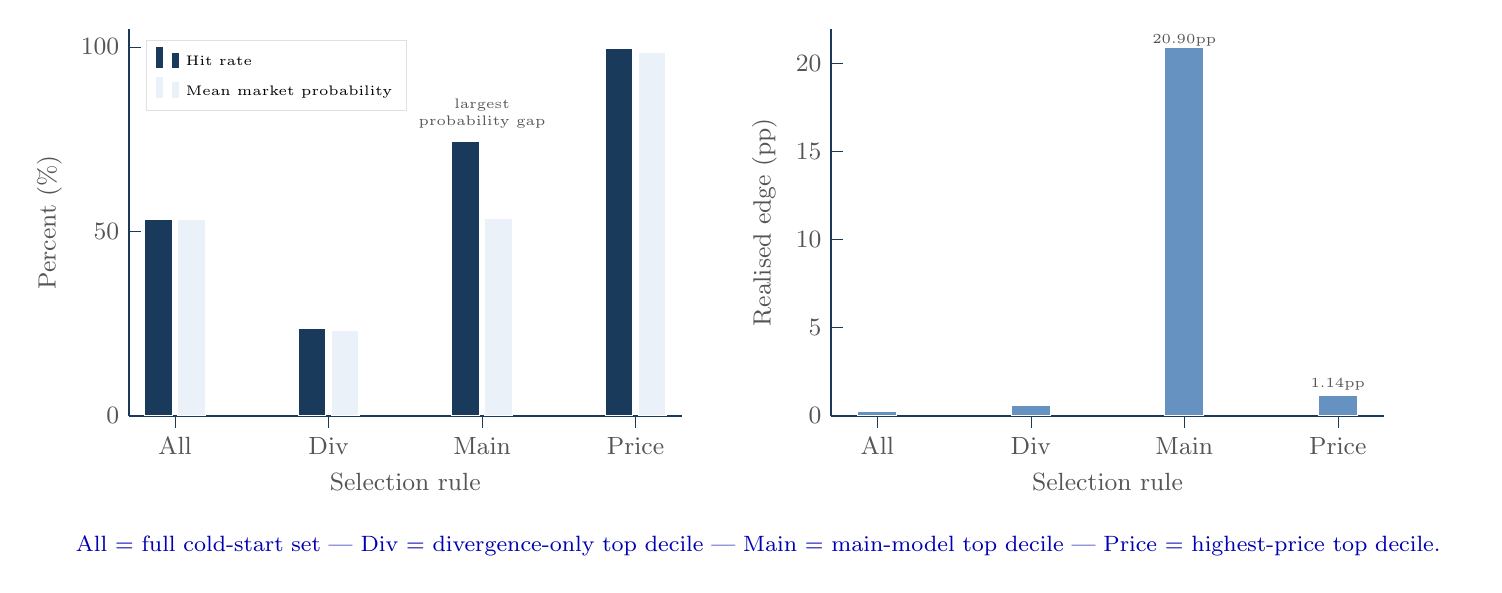
\begin{tikzpicture}
\begin{groupplot}[
  group style={group size=2 by 1, horizontal sep=1.9cm},
  fig style,
  width=8.6cm,
  height=6.5cm,
]
\nextgroupplot[
  ybar,
  bar width=10pt,
  ymin=0, ymax=105,
  symbolic x coords={All,Div,Main,Price},
  xtick=data,
  xticklabels={All,Div,Main,Price},
  ylabel={Percent (\%)},
  xlabel={Selection rule},
%  title={Hit Rate vs.\ Market Probability},
  title style={font=\tiny\bfseries, text=fignavy},
  tick label style={font=\small},
  ylabel style={font=\small},
  xlabel style={font=\small},
  legend style={font=\tiny, draw=black!12, fill=white, at={(0.03,0.97)}, anchor=north west},
  legend cell align=left,
]
\addplot[ybar, fill=fignavy, draw=white] coordinates {
  (All,53.34) (Div,23.77) (Main,74.43) (Price,99.52)
};
\addlegendentry{Hit rate}
\addplot[ybar, fill=figlblue!60!white, draw=white] coordinates {
  (All,53.11) (Div,23.18) (Main,53.53) (Price,98.38)
};
\addlegendentry{Mean market probability}
\node[text=figgrey, font=\tiny, align=center] at (axis cs:Main,82) {largest\\probability gap};

\nextgroupplot[
  ybar,
  bar width=14pt,
  ymin=0, ymax=22,
  symbolic x coords={All,Div,Main,Price},
  xtick=data,
  xticklabels={All,Div,Main,Price},
  ylabel={Realised edge (pp)},
  xlabel={Selection rule},
%  title={Realised Edge},
  title style={font=\tiny\bfseries, text=fignavy},
  tick label style={font=\small},
  ylabel style={font=\small},
  xlabel style={font=\small},
]
\addplot[ybar, fill=figblue!85!white, draw=white] coordinates {
  (All,0.23) (Div,0.59) (Main,20.90) (Price,1.14)
};
\node[text=figgrey, font=\tiny] at (axis cs:Main,21.3) {\edit{20.90pp}};
\node[text=figgrey, font=\tiny] at (axis cs:Price,1.8) {1.14pp};
\end{groupplot}

\node[anchor=north,text=ucdblue,font=\footnotesize, align=center, text width=18.0cm]
  at ($(group c1r1.south west)!0.5!(group c2r1.south east)+(0,-1.4cm)$)
  {All = full cold-start set | Div = divergence-only top decile  |  Main = main-model top decile  |  Price = highest-price top decile.};
\end{tikzpicture}

\vspace{-0.75em}
\caption{Economic screening diagnostics.}
\label{fig:screening_diagnostics}
\end{figure}

The main-model top decile creates a large gap between realised hit rate and market-implied probability, while the highest-price benchmark delivers a high raw hit rate but very little edge and the divergence-only benchmark is nearly flat.

\vspace{-0.75em}
\subsection{Friction, sizing and deployability}

\edit{We use a simple friction sensitivity check on the top-alpha slice. After applying a min market-volume filter, a \$500 position cap and a 0.5\% participation limit, 2,195 of 2,276 top-alpha trades remain.}

We stress-test at up to $150$~bps even though Polymarket's on-chain
CLOB has effectively zero protocol fees and gas costs of the order of
cents on Polygon, in order to absorb unmodelled slippage on illiquid
contracts and any future protocol fee changes.

\begin{table}[H]
\centering
\small
\begin{tabular}{lrrrr}
\toprule
Screen & Trades & Net edge/share & Mean net ROI & Median effective stake (\$) \\
\midrule
\edit{Top 10\% alpha, 0 bps cost}   & \edit{2,195} & \edit{0.2137} & \edit{0.4125} & \edit{41.76} \\
\edit{Top 10\% alpha, 50 bps cost}  & \edit{2,195} & \edit{0.2087} & \edit{0.4014} & \edit{41.76} \\
\edit{Top 10\% alpha, 150 bps cost} & \edit{2,195} & \edit{0.1987} & \edit{0.3793} & \edit{41.76} \\
\bottomrule
\end{tabular}
\caption{Friction sensitivity on the filtered top-alpha slice.}
\label{tab:friction}
\end{table}

% --------------------------------------
% FIGURE: Friction sensitivity curve
% LEFT: gross edge (flat) vs net edge (declining) line chart
% RIGHT: net ROI bar chart at each cost level
% Edit: gross_edge constant, cost coordinates, y-axis limits
% --------------------------------------
\begin{figure}[H]
\centering
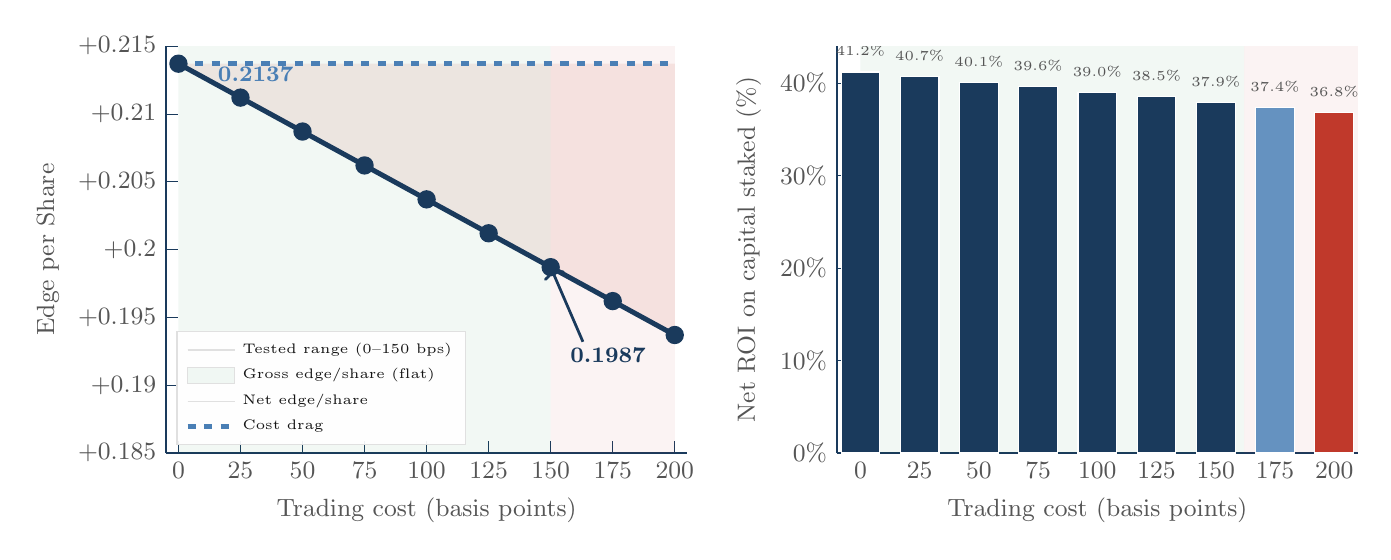
\begin{tikzpicture}
\begin{groupplot}[
  group style={group size=2 by 1, horizontal sep=1.9cm},
  fig style,
  width=8.2cm,
  height=6.75cm,
]

\nextgroupplot[
  %title={Edge per Share vs.\ Cost},
  title style={font=\tiny\bfseries, text=fignavy},
  xmin=-5, xmax=205,
  ymin=0.185, ymax=0.215,
  xtick={0,25,50,75,100,125,150,175,200},
  ylabel={Edge per Share},
  xlabel={Trading cost (basis points)},
  ytick={0.185,0.190,0.195,0.200,0.205,0.210,0.215},
  yticklabel={+\pgfmathprintnumber[fixed,precision=3]{\tick}},
  tick label style={font=\small},
  ylabel style={font=\small},
  xlabel style={font=\small},
  legend style={font=\tiny, draw=black!12, fill=white, fill opacity=0.92, at={(0.02,0.02)}, anchor=south west},
  legend cell align=left,
]
\addplot[draw=none, fill=figgreen, fill opacity=0.06] coordinates {
  (0,0.185) (150,0.185) (150,0.215) (0,0.215)
} \closedcycle;
\addlegendimage{area legend, draw=none, fill=figgreen, fill opacity=0.06}
\addlegendentry{Tested range (0--150 bps)}

\addplot[draw=none, fill=figred, fill opacity=0.06] coordinates {
  (150,0.185) (200,0.185) (200,0.215) (150,0.215)
} \closedcycle;

\addplot[name path=grossedge, figblue, dashed, line width=1.6pt] coordinates {
  (0,0.2137) (200,0.2137)
};
\addlegendentry{Gross edge/share (flat)}

\addplot[name path=netedge, fignavy, line width=1.8pt, mark=*, mark size=2.4pt] coordinates {
  (0,0.2137) (25,0.2112) (50,0.2087) (75,0.2062) (100,0.2037)
  (125,0.2012) (150,0.1987) (175,0.1962) (200,0.1937)
};
\addlegendentry{Net edge/share}

\addplot[draw=none, fill=figred, fill opacity=0.10] fill between[of=grossedge and netedge];
\addlegendentry{Cost drag}

\node[text=figblue, font=\footnotesize\bfseries, anchor=west] at (axis cs:12,0.2129) {\edit{0.2137}};
\draw[->, line width=1.0pt, color=fignavy] (axis cs:163,0.1932) -- (axis cs:150,0.1987);
\node[text=fignavy, font=\footnotesize\bfseries, anchor=west] at (axis cs:154,0.1922) {\edit{0.1987}};

\nextgroupplot[
  %title={Net ROI vs.\ Cost},
  title style={font=\tiny\bfseries, text=fignavy},
  xmin=-10, xmax=210,
  ymin=0, ymax=44,
  xtick={0,25,50,75,100,125,150,175,200},
  ytick={0,10,20,30,40},
  yticklabel={\pgfmathprintnumber[fixed,precision=0]{\tick}\%},
  ylabel={Net ROI on capital staked (\%)},
  xlabel={Trading cost (basis points)},
  tick label style={font=\small},
  ylabel style={font=\small},
  xlabel style={font=\small},
]
\addplot[draw=none, fill=figgreen, fill opacity=0.06] coordinates {
  (0,0) (162,0) (162,44) (0,44)
} \closedcycle;
\addplot[draw=none, fill=figred, fill opacity=0.06] coordinates {
  (162,0) (210,0) (210,44) (162,44)
} \closedcycle;

% Values from notebook Cell 32: 0bps=41.20%, 25bps=40.64%, 50bps=40.08%, 100bps=38.96%, 150bps=37.84%
% Interpolated at 75, 125, 175, 200 bps (slope = -0.0224% per bps)
\addplot[ybar, bar width=14pt, fill=fignavy, draw=white] coordinates {
  (0,41.2) (25,40.7) (50,40.1) (75,39.6) (100,39.0) (125,38.5) (150,37.9)
};
\addplot[ybar, bar width=14pt, fill=figblue!85!white, draw=white] coordinates {(175,37.4)};
\addplot[ybar, bar width=14pt, fill=figred, draw=white] coordinates {(200,36.8)};
\node[text=figgrey, font=\tiny] at (axis cs:0,41.2)  [above=2pt] {\edit{41.2\%}};
\node[text=figgrey, font=\tiny] at (axis cs:25,40.7)  [above=2pt] {\edit{40.7\%}};
\node[text=figgrey, font=\tiny] at (axis cs:50,40.1)  [above=2pt] {\edit{40.1\%}};
\node[text=figgrey, font=\tiny] at (axis cs:75,39.6)  [above=2pt] {\edit{39.6\%}};
\node[text=figgrey, font=\tiny] at (axis cs:100,39.0) [above=2pt] {\edit{39.0\%}};
\node[text=figgrey, font=\tiny] at (axis cs:125,38.5) [above=2pt] {\edit{38.5\%}};
\node[text=figgrey, font=\tiny] at (axis cs:150,37.9) [above=2pt] {\edit{37.9\%}};
\node[text=figgrey, font=\tiny] at (axis cs:175,37.4) [above=2pt] {\edit{37.4\%}};
\node[text=figgrey, font=\tiny] at (axis cs:200,36.8) [above=2pt] {\edit{36.8\%}};

%\node[text=figgreen!80!black, font=\small\itshape] at (axis cs:77,1.8) {Tested range};
\end{groupplot}

%\node[anchor=south, text=fignavy, font=\normalsize\bfseries, align=center]
%  at ($(group c1r1.north west)!0.5!(group c2r1.north east)+(0,0.85cm)$)
%  {Friction Sensitivity: Top-10\% Alpha Slice (2,179 trades after filters)};

%\node[anchor=north, text=figgrey, font=\footnotesize\itshape, align=center, text width=13.4cm]
%  at ($(group c1r1.south west)!0.5!(group c2r1.south east)+(0,-0.95cm)$)
%  {ROI~$=$~(outcome\_correct $-$ avg\_price $-$ cost) $\div$ avg\_price. At the median \$41.16 stake, each extra 25\,bps reduces net ROI by about 0.56 percentage points.};
\end{tikzpicture}

\vspace{-0.75em}
\caption{\edit{Friction sensitivity on the top-10\% alpha slice (2,195 trades after filters)}}
\label{fig:friction}
\end{figure}

\[
ROI= \frac{\text{(outcome\_correct)} - \text{(avg\_price)} - \text{(cost)}}{ \text{avg\_price}}
\]
At the \edit{median \$41.76} stake, each extra 25\,bps reduces net ROI by about 0.56 percentage points.\\

Left: \edit{gross edge per share (dashed, flat at 0.2137)} versus net edge after costs from 0 to 200 bps;
the green band marks the range tested in the notebook (0--150 bps). Right: net ROI on capital
staked at each cost level. \edit{At 150 bps the net ROI remains at 37.9\%, well above breakeven.}

\subsection{Risk-adjusted performance}

A raw ROI figure is insufficient for a financial application. The strategy must also be evaluated on its risk-adjusted return profile. \edit{The analysis below is applied to the 2,195 trades in the filtered top-10\% alpha slice,} using per-trade P\&L computed as $\text{P\&L}_i = (\text{shares}_i) \times (\text{outcome}_i - \text{price}_i)$ where $\text{shares}_i = \text{stake}_i \div \text{price}_i$.

\begin{table}[H]
\centering
\small
\begin{tabular}{lrr}
\toprule
Risk metric & Value & Notes \\
\midrule
Mean per-trade P\&L         & \$\MeanTradePnl  & Across \FilteredRows\ filtered trades \\
Std dev of per-trade P\&L   & \$\StdTradePnl  & Reflects the binary payoff structure and stake sizing \\
Per-trade Sharpe ratio       & \TradeSharpe     & Mean ROI / std ROI, trade-level \\
VaR (95\%, per trade)       & \$\TradeVaR    & 5th percentile of the per-trade P\&L distribution \\
CVaR (95\%, per trade)      & \$\TradeCVaR    & Mean loss conditional on the worst 5\% of trades \\
Maximum portfolio drawdown   & \$\MaxDrawdownUSD  & Peak-to-trough on cumulative filtered-slice P\&L \\
Max drawdown (\% of peak)    & \MaxDrawdownPct\%    & Drawdown relative to prior cumulative peak \\
Total gross P\&L (7 months) & \$\GrossPnlSevenMonths & At the \$500 base position cap \\
\bottomrule
\end{tabular}
\caption{\edit{Risk-adjusted performance metrics for the top-10\% alpha slice (2,195 trades, September 2025 to April 2026). Sharpe is computed at the trade level; see notebook for the full distributional calculation.}}
\label{tab:risk}
\end{table}

\begin{figure}[H]
\centering
\includegraphics[width=\linewidth]{figures/risk_adjusted_profile.png}
\caption{Risk profile for the filtered top-10\% alpha slice. Left: cumulative P\&L in chronological trade order with drawdown shading. Right: per-trade net P\&L distribution with mean and 95\% VaR markers.}
\label{fig:riskprofile}
\end{figure}

The filtered slice has a positive but not trivial risk profile. A trade-level Sharpe of \TradeSharpe\ is economically meaningful rather than exceptional, while the 95\% VaR/CVaR of \$\TradeVaR/\$\TradeCVaR\ and maximum drawdown of \MaxDrawdownPct\% show that downside clustering still occurs even after screening. This is consistent with a selective, size-controlled decision-support overlay rather than a fully automated high-leverage strategy.

\paragraph{Annualisation and the right unit for Sharpe.}
A trade-level Sharpe of \edit{$0.396$} is deliberately not annualised. With
\edit{$314$} qualifying trades per month (\edit{$\approx 3{,}763$} per year), naive
$\sqrt{N}$ annualisation would give
\edit{$0.396 \times \sqrt{3{,}763} \approx 24.3$}, which is economically
implausible and confirms that trade-level Sharpe is the appropriate
unit for a binary bet-by-bet strategy where each trade is a discrete
independent event rather than a step in a continuously compounded
return series. We therefore retain the per-trade figure throughout
Section~\ref{sec:business}; readers accustomed to the
``annualised Sharpe $>1$'' convention should interpret \edit{$0.396$} as
meaningful edge per deployed ticket, not as a direct comparator to a
continuously-held equity strategy.

\subsection{AUM scaling and commercial income estimate}

%To assess commercial viability, the strategy is scaled to a realistic institutional allocation. 
The evaluation period runs from September 2025 to April 2026 (approx 7 months), during which \TradesPerMonth\ qualifying trades per month passed the top-alpha and liquidity filters. Assuming an average market resolution time of 30 days, the strategy requires approximately \TradesPerMonth\ simultaneously open positions at any point in time, implying peak capital deployment of roughly \$\PeakCapitalUSD\ at the \$500 position cap. \edit{A fund allocating \textbf{\$1M} to this strategy would therefore operate with a comfortable 6.4$\times$ buffer above peak deployment.}

\begin{table}[H]
\centering
\small
\begin{tabular}{rrrr}
\toprule
AUM allocation & Cap per Trade&Annualised gross P\&L & Net of team cost (\euro{}480k) \\
\midrule
\$1M & \$500  & \$\AnnualPnlOneM & $-$\euro{}\NetTeamOneM \\
\$5M & \$2{,}500 & \$\AnnualPnlFiveM & $+$\euro{}\NetTeamFiveM \\
\$10M & \$5{,}000 & \$\AnnualPnlTenM & $+$\euro{}\NetTeamTenM \\
\bottomrule
\end{tabular}
\caption{Estimated annualised P\&L at three AUM scales.}
\label{tab:aum}
\end{table}

\edit{Annualised gross P\&L is calculated as $\$\GrossPnlSevenMonths \times (\frac{12}{7}) \approx \$\AnnualPnlOneM$ at the \$500 cap. Larger AUM is then scaled using the notebook's conservative liquidity-adjusted multipliers rather than pure linear extrapolation: \FiveMScale$x$ for the \$2{,}500 cap and \TenMScale$x$ for the \$5{,}000 cap. These are scenario assumptions anchored to the observed 0.5\% volume constraint, not exact algebraic identities.}

\subsection{Justification for a team of four}

\edit{For argument's sake, we can say a dedicated four-person data science team in Ireland commands a blended all-in cost of approximately \euro{}120k per person pa giving a total annual team budget of \euro{}480k (approximately \$518k under the notebook's 1.08 USD/EUR assumption). Beyond direct return, the team still contributes indirect value through systematic risk control, ongoing model maintenance, and institutional process credibility, but the quantitative break-even point under the updated hard-coded business case remains \$5M rather than \$1M.}

\subsection{Recommended use in practice}

The most realistic business use is a decision-support overlay: restrict attention to the top 10--20\% of model-alpha trades, require minimum liquidity and hard position limits, retrain on an expanding window with monthly calibration checks, and use the score alongside human judgement rather than as a fully automated execution rule.

\subsection{Key business risks}

From a business perspective, four risks remain:
\begin{itemize}[label=--]
    \item \textbf{Execution risk:} actual fills, slippage and queue position are not observed in the notebook.
    \item \textbf{Regime risk:} the evaluation period is limited, so the edge may weaken if market structure or participant behaviour changes.
    \item \textbf{Coverage risk:} the analysis is restricted to resolved geopolitical buy-side trades, not the full Polymarket universe.
    \item \textbf{Model risk:} some gains are modest relative to a strong benchmark, so careless overtrading could eliminate the benefit.
\end{itemize}

\begin{mdframed}[linewidth=0.6pt, backgroundcolor=ucdblue]
\vspace{0.75em}
\textcolor{white}{\textbf{Business conclusion.} The model has real commercial value as a screening and ranking engine. It identifies a small, higher-conviction set of trades that outperform market pricing even for previously unseen wallets. The correct business recommendation is selective deployment with tight limits, not immediate full automation.}
\vspace{0.75em}
\end{mdframed}

\newpage
% =========================================================
\appendix
\section{Appendix}
% =========================================================

\subsection{DB Query for Pulling Polymarket Event \& Wallet Data}
\label{sec:DB_Query}
\begin{minted}[mathescape,linenos,numbersep=5pt,frame=lines,framesep=2mm]{sql}
    SELECT
        t.timestamp,
        t.wallet,
        t.side,
        t.outcomes                                           AS bet_outcome,
        t.usd_amount,
        t.token_amount,
        t.price,
        t.condition_id,
        t.transactionHash                                    AS transaction_hash,
        DATEDIFF('hour', t.timestamp, m.closedTime)          AS hours_before_resolution,
        CASE
            WHEN t.side = 'BUY' AND t.outcomes = 'Yes' AND t.price < 0.5 THEN 1
            WHEN t.side = 'BUY' AND t.outcomes = 'No'  AND t.price < 0.5 THEN 1
            ELSE 0
        END                                                  AS bet_vs_market,
        CASE WHEN t.outcomes = m.resolvedOutcome THEN 1 ELSE 0 END AS outcome_correct,
        CASE WHEN t.outcomes = 'Yes' THEN 1 ELSE -1 END     AS wallet_direction,
        m.closedTime                                         AS resolution_date,
        m.endDate                                            AS market_end_date,
        m.question,
        m.volume                                             AS market_volume,
        m.tags                                               AS tags
    FROM trades t
    JOIN markets m ON t.condition_id = m.conditionId
    WHERE
        m.resolvedOutcome IN ('Yes', 'No')
        AND m.closedTime IS NOT NULL
        AND t.side = 'BUY'
\end{minted}

\subsection{HHI Computation}
\label{sec:hhi_append}
For wallet $w$ with tag shares $s_{w,t}$, $\text{HHI}_w = \sum_t s_{w,t}^2$, where $\text{HHI}=1$ indicates a wallet whose volume is entirely in one tag and $\text{HHI}\to 0$ indicates a wallet diversified across many tags. 

\subsection{The Brier Statistic}
We want to give a short note on the Brier test stat, given it plays a central role in model selection in Section~\ref{sec:ml}. For a set of $N$ predictions, the formula is:
\[
BS = \frac{1}{N} \sum_{i=1}^{N} (f_i - o_i)^2
\]

Where:
\begin{itemize}[label=--]
    \item $f_i$ is the predicted probability of the event (e.g., $0.75$).
    \item $o_i$ is the actual outcome ($1$ if the event occurred, $0$ if it did not).
\end{itemize}

The score ranges from \textbf{0 to 1}:
\begin{itemize}[label=--]
    \item \textbf{0}: Perfect accuracy.
    \item \textbf{1}: Perfect inaccuracy.
    \item \textbf{0.25}: The score for a constant prediction of $0.5$ (50\% chance).
\end{itemize}

\subsection{\edit{Why Sharpe Ratio Isn't Annualised}}
\edit{A trade-level Sharpe of $0.396$ is deliberately not annualised. With
$314$ qualifying trades per month ($\approx 3{,}763$ per year), naive}
$\sqrt{N}$ annualisation would give
\[
0.396 \times \sqrt{3{,}763} \approx 24.3
\] 
\edit{which is economically implausible and confirms that trade-level Sharpe is the appropriate}
unit for a binary bet-by-bet strategy where each trade is a discrete
independent event rather than a step in a continuously compounded
return series. We therefore retain the per-trade figure throughout
Section~\ref{sec:business}. \edit{If you're accustomed to the}
``annualised Sharpe $>1$'' convention should interpret \edit{$0.396$} as
meaningful edge per deployed ticket, not as a direct comparator to a
continuously-held equity strategy.



\subsection{\edit{Interpretation of the liquidity multipliers.}}
\edit{The $4.9\times$ and $9.0\times$ scaling factors in Table~\ref{tab:aum} should be read as conservative scenario assumptions taken from the saved notebook, not as exact algebraic extrapolations. The empirical support for these assumptions is that approximately $52.5\%$ of evaluation-period markets have volume above $\$500{,}000$ and approximately $41.2\%$ have volume above $\$1\text{M}$, which is consistent with scaling that is materially sub-linear once the 0.5\% participation cap is imposed. Because actual fill quality also depends on queue position, overlap of open trades, and market-by-market execution frictions, the notebook multipliers are best interpreted as disciplined business-case scenarios rather than precise estimators.}

\subsection{From per-trade to portfolio VaR.}
The VaR and CVaR figures in Table~\ref{tab:risk} are per-trade
USD. At the typical deployment of $\sim 311$ simultaneously open
positions, $\sqrt{N}$ diversification gives a portfolio standard
deviation of 
\[
\$219.57 \times \sqrt{311} \approx \$3{,}870
\] 
and a one-sided $95\%$ portfolio VaR of approx
$1.65\sigma \approx \$6{,}380$. This is small relative to the
implied $\$155{,}643$ peak deployed capital, so the portfolio-level
downside does not materially constrain the $\$1\text{M}$ allocation
beyond the per-trade controls already imposed.

% =========================================================
\section{\edit{Bibliography}}
% =========================================================

\begin{thebibliography}{9}
\bibitem{chen2016xgboost}
\edit{Chen, T. and Guestrin, C. (2016). XGBoost: A scalable tree boosting system. In \emph{Proceedings of the 22nd ACM SIGKDD International Conference on Knowledge Discovery and Data Mining}, 785--794.}

\bibitem{lundberg2017shap}
\edit{Lundberg, S. M. and Lee, S.-I. (2017). A unified approach to interpreting model predictions. In \emph{Advances in Neural Information Processing Systems}, 4765--4774.}

\bibitem{polymarket}
\edit{Polymarket (n.d.). Platform and market documentation. Available from the Polymarket website and public market interface.}
\end{thebibliography}

\end{document}
